\documentclass[12pt,a4paper,openright,twoside]{book}
\usepackage[utf8]{inputenc}
\usepackage{disi-thesis}
\usepackage{code-lstlistings}
\usepackage{notes}
\usepackage{shortcuts}
\usepackage{acronym}

\school{\unibo}
\programme{Corso di Laurea Magistrale in Ingegneria e Scienze Informatiche}

\title{EleKtion: \\
una Libreria Kotlin Multiplatform \\
per la Democrazia Digitale \\
in Nuovi Contesti \\
}
\author{Jacopo Corina}
\date{\today}
\subject{Laboratorio Di Sistemi Software}
\supervisor{Prof. Danilo Pianini}
\session{IV Appello della}
\academicyear{2022-2023}

% Definition of acronyms
\acrodef{IoT}{Internet of Thing}
\acrodef{vm}[VM]{Virtual Machine}

\acrodef{gh}[GH]{GitHub}

\acrodef{gha}[GH Actions]{GitHub Actions}

\acrodef{ghpages}[GH Pages]{GitHub Pages}

\acrodef{ghpackages}[GH Packages]{GitHub Packages}

\acrodef{ci}[CI]{Continuous Integration}

\acrodef{cd}[CD]{Continuous Delivery}

\acrodef{dsl}[DSL]{Domain Specific Language}
\acrodef{f1}[F1]{Formula 1}

\acrodef{npm}[NPM]{Node Package Manager}

\acrodef{jvm}[JVM]{Java Virtual Machine}

\acrodef{js}[JS]{Javascript}


\mainlinespacing{1.3} % line spacing in mainmatter, comment to default (1)

\begin{document}

\frontmatter 
\frontispiece

\begin{abstract}	
    La tesi si concentra sull'evoluzione della democrazia digitale e l'implementazione di EleKtion, una libreria multipiattaforma per votazioni. 
    Dopo un' introduzione sulla definizione di democrazia, si analizzano le caratteristiche delle votazioni 
    e si progetta un linguaggio di dominio volto a facilitare la definizione del contesto della votazione.
    La fase di implementazione si svolge affrontando aspetti cruciali come la gestione degli artefatti 
    e l'implementazione dei casi di test. 
    In seguito si sperimenta la libreria utilizzando dati reali delle competizioni di Formula 1,
    evidenziando come logiche algoritmiche personalizzabili possano generare esiti alternativi, confrontandoli infine 
    con quelli reali per una valutazione qualitativa del sistema.
\end{abstract}

\begin{dedication} % this is optional
Ai miei genitori
\end{dedication}


%----------------------------------------------------------------------------------------
\tableofcontents   
\listoffigures     % (optional) comment if empty
\lstlistoflistings % (optional) comment if empty
%----------------------------------------------------------------------------------------

\mainmatter

%----------------------------------------------------------------------------------------
\chapter{Introduzione}
\label{chap:introduction}
Nell'ultimo ventennio l'informatica sta perpetuando un progresso tecnologico sempre più pervasivo
nella quotidianità delle persone, digitalizzando i processi in numerosi ambiti, come le procedure burocratiche,
la razionalizzazione delle risorse, la raccolta di opinioni di una comunità,
con la tendenza di giungere ad una semplificazione e ad una maggior diffusione sulle informazioni di
interesse per gli \textit{stakeholders}.
Questo fenomeno ha impattato, pur con qualche difficoltà, anche uno dei processi che tradizionalmente
è più legato ad una lavorazione analogica e ad una maggior attenzione da parte del pubblico,
ossia il contesto delle votazioni e dell'applicazione del potere democratico all'interno di uno Stato.
L'informatizzazione delle votazioni è stata adattata a molteplici contesti, dalle votazioni per le  
elezioni dei rappresentanti politici a decisioni interne tra gruppi di lavoro e consultazioni
della volontà popolare. L'espansione potrà in futuro coinvolgere nuovi settori, come quello sportivo, ponendo sugli esiti una maggior
influenza fondata su nuovi criteri e volontà popolari.
Lo scopo della tesi è realizzare una libreria in \texttt{Kotlin Multiplatform} chiamata EleKtion, la quale permette di creare e gestire
votazioni lasciando all'utilizzatore la possibilità di parametrizzazione.
La disponibilità degli artefatti finali su molteplici piattaforme permette di massimizzarne la diffusione, garantendo
allo stesso tempo che il prodotto sia stato generando seguendo criteri di qualità, sia a livello di logiche di funzionamento
che correttezza sintattica del codice sorgente.
In questa tesi viene presentata inizialmente una panoramica relativa alla nascita della democrazia, di come essa è mutata nel tempo,
e di come l'approccio informatico può, e in certi casi ha potuto, riportare maggior potere nella volontà popolare, abbattendo barriere
geografiche e sociali.
Successivamente viene mostrata l'analisi e la modellazione del dominio per la gestione delle votazioni,
approfondendo le differenti tipologie di voto.
Viene poi esposta la progettazione di un linguaggio di dominio utile a definire con maggior facilità il contesto della votazione,
generando diagrammi UML architetturali, per poi vagliare gli aspetti implementantivi della libreria, 
partendo dagli strumenti che semplificano l'evoluzione e la pubblicazione del software fino ad arrivare ai casi di test.
Infine, viene illustrata una sperimentazione della libreria utilizzando dati relativi a campionati sportivi, nello specifico
scegliendo come sport la Formula 1. L'applicazione di logiche algoritmiche, definibili dall'utilizzatore, e la possibilità
di dichiarare elenchi di voti nelle gare, pongono nuovi scenari che possono modificare e mutare la storia di un campionato.
Questi risultati vengono confrontati con quelli reali per ottenere un'evidenza utile ad una valutazione qualitativa.


%----------------------------------------------------------------------------------------
\chapter{Democrazia Digitale}
Il termine \textit{Democrazia}, derivante dal greco \textit{démos krátos} (governo del popolo),
indica una forma di governo nella quale il potere appartiene al popolo ed è esercitato attraverso forme dirette, che coinvolgono attivamente
i cittadini, e attraverso forme rappresentantive, che prevedono un sistema di rappresentanza rinnovata ciclicamente
attraverso apposite elezioni.
In una qualunque forma di \textit{democrazia}, sono fondamentali i principi di elezioni libere, equità dei cittadini, partecipazione
attiva alla vita politica, protezione dei diritti fondamentali e della libertà personale attraverso costituzioni~\cite{vinod2017state}.
Nelle epoche successive alle prime forme di democrazia "unanime" (per quanto il concetto di cittadinanza fosse assai diverso da quello attuale,
ad esempio, erano escluse donne, schiavi e minori di 20 anni), complice la complessità
delle materie da amministrare e il numero crescente di partecipanti fisici, la democrazia
rappresentativa ha preso la maggior diffusione. 
La modernizzazione tecnologica accelerata di recente con l'avvento della pandemia da Covid-19, che ha evidenziato notevoli problemi
logistici tra cui la gestione del distanziamento~\cite{sotoacosta}, ha riacceso l'opportunità di
permettere il ritorno ad un controllo più diretto da parte della collettività.

La \textit{democrazia digitale} (o \textit{e-democracy}) è definibile come "l'esercizio di processi decisionali democratici attraverso 
l'uso di informazioni e tecnologie abilitanti alla comunicazione, in particolare Internet"~\cite{rotzocki}.
Queste tecnologie, abilitanti a superare limitazioni territoriali e sociali,
facilitano l'esercizio di ulteriori forme di democrazia,
come quella partecipata, in cui i cittadini, piuttosto che
sostituirsi ai rappresentanti, forniscono idee sullo sviluppo dell'indirizzo di governo
permettendo così di creare un collettore di confronto ed analisi di situazioni disomogenee.
Nonostante la virtualizzazione della partecipazione permetterebbe alle fasce più disagiate di essere
maggiormente coinvolte, introduce allo stesso tempo un motivo di scetticismo relativo alla componente tecnologica
in ambito di sicurezza informatica, usabilità, segretezza e manipolazione del voto~\cite{aichholzer2020experience}.
Stabilire un legame di fiducia con queste tecnologie, normarne la verificabilità e pattuire principi di 
\textit{accountability} sono i fattori principali e quindi pre-condizioni essenziali
per una diffusione efficace. 
Alcuni autori sostengono che è impossibile avere leggitimità in quanto "la natura dei computer è tale che il loro funzionamento interno è segreto.
Poiché le transazioni e i calcoli avvengono a livello elettronico, 
non è fisicamente possibile per gli esseri umani osservare esattamente ciò che un computer sta facendo"~\cite{mcgaley}.
L'applicazione più comune di queste tecnologie emergenti è legata al mondo della politica~\cite{aichholzer2020experience}:
sono degni di nota casi come l'Estonia, che dal 2005 rende possibili via Internet le votazioni
per elezioni e referendum, e la Svizzera, che dal 2015 rende progressivamente disponibile la possibilità di votare online
ai cittadini, sulla base delle regole operative che i Cantoni decidono seguendo le linee guida dettate 
dalla Confederazione Svizzera.
In Italia possiamo rilevare l'applicativo PartecipaMi\footnote{\url{https://archive.is/HIXoC}},
organizzato per mettere in contatto la popolazione milanese con l'amministrazione comunale.
Inoltre, queste soluzioni sono spesso adottate da partiti o movimenti politici per avviare iniziative
e votazioni interne tra i membri, come nel caso del Partito Pirata tedesco in Germania (piattaforma LiquidFeedback),
o il Movimento 5 Stelle in Italia (piattaforma Rousseau). Lo scopo principale è quello di promuovere la discussione
di proposte tra i membri di un organizzazione, le quali saranno portate in sede legislativa da un loro rappresentante~\cite{korthagen2020non}.
Sistemi come LiquidFeedback, OpenDCN, Airesis, essendo strutturati come applicativi end-to-end,
pongono molta enfasi sull'interazione tra utenti, la presentazione e validazione di proposte,
l'eventuale presenza di deleghe, l'espressione del voto tramite una lista di preferenze, ma
non permettono la variazione delle logiche da applicare per la selezione del vincitore~\cite{Trapanese:2018}.
In altri sistemi, una fase di analisi iniziale poco trasversale ha portato a dar molto risalto
ad aspetti non funzionali, come la privacy, e scarsità di approfondimento per quelli funzionali, come il modello di democrazia
da applicare, che per alcuni aspetti rimane implicito~\cite{Pianini:2019}.
Ciò è dovuto anche al fatto che il maggior coinvolgimento si concentra 
principalmente alle fasi iniziali e finali del ciclo della votazione~\cite{hennen2020european}.
La mancanza di elementi formalizzanti, che descrivono dettagliatamente tutti gli step applicati nel
processo, unita alle variazioni ed evoluzioni che vengono apportate nel tempo, portano alla divergenza del flusso rispetto all'idea iniziale, 
che conseguentemente non risulterà chiaro agli utilizzatori e potenzialmente potrebbe scoraggiare l'utilizzo del sistema~\cite{Pianini:2019}.

Al di là dell'applicazione di \textit{e-democracy} nel mondo della politica, che riscontra
ostacoli legati più all'aspetto organizzativo ed umano che ad aspetti di evoluzione tecnologica,
vi sono esempi notabili anche nel campo del \textit{pervasive computing}, ad esempio nell'ambito delle \textit{smart cities}.
Ricollegandosi al fenomeno dei cambiamenti climatici che stanno inesorabilmente continuando ad avanzare,
in certe zone del mondo l'acqua potabile sta diventando un bene sempre meno reperibile e degno di salvaguardia.
In~\cite{smartwater} si pone il focus sull'adozione di sistemi di \textit{IdroInformatica}. Questo tipo di sistema permette di analizzare 
e monitorare, attraverso sensori e componenti real-time \texttt{SCADA} (Supervisory Control And Data Acquisition), gli attuali flussi e pressioni nella
rete di distribuzione ed effettuare predizioni sui futuri guasti. Questi strumenti di analisi possono fornire ai cittadini
indicazioni su come ottimizzare l'utilizzo delle risorse. L'unione di questi sistemi ad un coinvolgimento digitale e democratico,
che porti i cittadini a prendere parte alle decisioni per i cambiamenti della gestione presente in una determinata area,
permetterebbe una miglior localizzazione circa le soluzioni da intraprendere, ed ai cittadini una maggior consapevolezza, in quanto sono i principali \textit{stakeholders}, 
oltre ad attribuirli maggior responsabilità.
In altri Stati, come Canada e Paesi Bassi, la gestione dell'acqua è delegata ad iniziative locali che promuovono la collaborazione tra soggetti pubblici e privati.
Questi nuovi approcci alla gestione democratica degli interessi dei cittadini migliorano i rapporti di trasparenza e fiducia reciproca, permettendo una maggior capacità di espressione
verso i rappresentanti ma anche da parte di chi ora è in grado di recepire, in ottica di miglioramento continuo,
le esigenze del mondo "reale". 
L'intermediazione, applicata a questi nuovi contesti, continua a rimanere essenziale.
Piuttosto che diventare un nuovo "medium" per imporre decisioni, risulta più efficace per
favorire lo scambio costruttivo, mantenendo comunque le opportune autonomie riguardo alle
decisioni finali, tutelando gli interessi collettivi e al contempo educando le persone a mantenere
la libertà di pensiero~\cite{castelfranchi2019problematic}.


%----------------------------------------------------------------------------------------

%----------------------------------------------------------------------------------------
\chapter{Analisi}
In questo capitolo viene descritta l'analisi sugli aspetti caratterizzanti la libreria multipiattaforma EleKtion.
Viene esposto un approfondimento sui tipi di voto
ed alcuni algoritmi applicabili per ciascun tipo; successivamente viene definito un 
elenco di requisiti fondamentali per le fasi successive e infine,
viene fornita una modellazione del dominio mediante diagramma UML.
\section{Votazioni a singola preferenza}
La tipologia di voto a singola preferenza impone al votante di effettuare una scelta tra un
numero definito di candidati. Al termine della votazione, tipicamente si adotta il criterio
della votazione maggioritaria: si contano i voti ottenuti da ciascun candidato, e colui che ottiene il
numero più elevato risulta vincitore. A seconda del contesto preso in considerazione,
è possibile avere più turni per diminuire di volta in volta il numero di candidati coinvolti.
Se si arriva ad un pareggio, è possibile effettuare un nuovo ballottaggio oppure adottare
criteri secondari, che variano in base al dominio trattato.
\section{Votazioni a lista di preferenze}
\label{chapter:votazionilistapreferenze}
La tipologia di voto a lista di preferenze non impone al votante di effettuare un'unica scelta,
bensì di fissare un ordinamento tra i candidati che parta dal minor favorito al maggior favorito 
o viceversa. Questa logica permette di conservare più contenuto informativo sulle preferenze
rispetto alla singola scelta, e offre anche un dettaglio di gradimento degli altri candidati.
Questo tipo di voto è stato introdotto inizialmente dall'algoritmo di Condorcet ed è stato adottato
anche nelle sue varianti. Di seguito viene data una spiegazione sul funzionamento dell'algoritmo
di Condorcet, e di un suo derivato, l'algoritmo di Schultze.
\subsection{Algoritmo di Condorcet}
L'algoritmo di Condorcet permette di estrarre un vincitore tra ${n}$ candidati,
applicando il criterio di maggioranza tra le coppie di candidati.
Si generano le possibili coppie, si confrontano e si valuta quale candidato batte tutti gli altri nello scontro di coppia. 
All'interno di una coppia, un candidato è vincitore se occupa una posizione preferenziale rispetto all'altro.
Di seguito viene riportato un esempio, supponendo di avere tre possibili candidati, A, B, C,
e 60 differenti votanti, che ordinano i candidati dalla posizione 1 alla posizione 3 dove la posizione 1 
indica la posizione di maggior preferenza.
Si ottengono delle liste di preferenze come rappresentato in tabella \ref{table:voticondorcet}, in cui
è mostrata l'occorrenza di ciascuna lista.

\renewcommand{\arraystretch}{1.5}
\begin{table}[H]
    \centering
    \begin{tabular}{|c|c|c|c|}
    \hline
    \multicolumn{1}{|l|}{Posizione 1} & \multicolumn{1}{|l|}{Posizione 2} & \multicolumn{1}{|l|}{Posizione 3} & \multicolumn{1}{l|}{Numero di occorrenze della lista } \\ \hline
    A & C & B & 23                              \\ \hline
    B & C & A & 19                              \\ \hline
    C & B & A & 16                              \\ \hline
    C & A & B & 2                               \\ \hline
    \end{tabular}
    \caption{Tabella delle liste di preferenze, con l'occorrenza di ciascuna lista}
    \label{table:voticondorcet}
\end{table}

Ora è possibile effettuare confronti tra le coppie, partendo ad esempio dalla coppia (B,C)
\begin{itemize}
    \item{Nella prima lista C è in una posizione favorevole rispetto a B, quindi C ottiene 23 punti}
    \item{Nella seconda lista B è in una posizione favorevole rispetto a C, quindi B ottiene 19 punti}
    \item{Nella terza lista C è in una posizione favorevole rispetto a B, quindi C ottiene 16 punti}
    \item{Nella quarta lista C è in una posizione favorevole rispetto a B, quindi C ottiene 2 punti}
\end{itemize}

Si ha che il candidato C batte il candidato B con un punteggio di 41 a 19.
Facendo i confronti tra le coppie (A,B) e (A,C) si ottiene che il candidato
B batte il candidato A con un punteggio di 35 a 25, e il candidato C batte il candidato
A con un punteggio di 37 a 23. Il risultato finale è quindi il seguente:
\begin{itemize}
    \item{Posizione 1: C}
    \item{Posizione 2: B}
    \item{Posizione 3: A}
\end{itemize} 

In alcuni casi il metodo di Condorcet può non portare ad alcun vincitore, presentando un ciclo e trovandosi, ad esempio, in una situazione 
in cui C $>$ B, B $>$ A, A $>$ C.
Le varianti del metodo di Condorcet ottimizzano l'algoritmo per minimizzare il rischio
di indeterminazione del vincitore.
Può accedere, in Condorcet come nelle sue varianti, di ottenere dei pareggi,
i quali avvengono quando due o più concorrenti pareggiano l'uno con l'altro ma 
battono tutti i restanti. La situazione di pareggio può essere gestita in vari
modi, ad esempio, estraendo il vincitore in modo casuale, valutando altri criteri
come la preferenza nei singoli voti (most first choice) oppure mantenendo il set di pareggio
senza effettuare alcuna azione.
Dato il risultato della votazione, è possibile definire l'utilità individuale come il grado
di soddisfazione del votante. Il grado di soddisfazione sarà tanto più alto 
quanto più vicino è il risultato rispetto al voto espresso.
Concludendo, l'algoritmo porta ad un risultato nel quale si tende a massimizzare
l'utilità per il maggior numero di votanti, ossia a massimizzare l'utilità
complessiva. 

\subsection{Algoritmo di Schultze}
L'algoritmo di Schultze, conosciuto anche come Schwartz Sequential Dropping (SSD),
è una variante di Condorcet basata sulla sommatoria del conteggio delle vittorie tra i concorrenti.
Ad esempio, nel caso in cui si hanno 3 candidati, A, B, C,
e questi vengono ordinati in una lista di preferenze dalla posizione 1 alla posizione 3 dove la posizione 1 
indica la posizione di maggior preferenza, si può avere il seguente risultato:
\begin{itemize}
    \item{Posizione 1: A}
    \item{Posizione 2: B}
    \item{Posizione 3: C}
\end{itemize}    
In questa lista A ottiene 2 punti, B ottiene 1 punto mentre C nessuno.
Riprendendo i voti presenti in tabella \ref{table:voticondorcet} e moltiplicando
i punti per il numero di occorrenze, si ottiene la situazione finale mostrata in tabella \ref{table:risultatischultze}

\begin{table}[H]
    \centering
    \begin{tabular}{|c|c|c|c|c|c|}
    \hline
    \multicolumn{1}{|l|}{concorrente} & \multicolumn{1}{|l|}{x 23} & \multicolumn{1}{|l|}{x 19} & \multicolumn{1}{l|}{x 16} & \multicolumn{1}{l|}{x 2} & \multicolumn{1}{l|}{Sommatoria} \\ \hline
    A & 2 & 0 & 0 & 1 & 48                              \\ \hline
    B & 0 & 2 & 1 & 0 & 54                              \\ \hline
    C & 1 & 1 & 2 & 2 & 78                             \\ \hline
  
    \end{tabular}
    \caption{Tabella delle sommatorie ottenute con l'applicazione dell'algoritmo di Schultze}
    \label{table:risultatischultze}
\end{table}
\newpage
Prendendo in considerazione le sommatorie in ordine decrescente, otteniamo, il seguente risultato:
\begin{itemize}
    \item{Posizione 1: C}
    \item{Posizione 2: B}
    \item{Posizione 3: A}
\end{itemize} 

Il risultato di Schultze non coincide sempre con il risultato di Condorcet.

\newpage
\section{Requisiti}
La libreria EleKtion fornisce la possibilità di creare ed effettuare votazioni.
Essa non tratta la parte preliminare ad una votazione, quale fase di proposta, discussione,
eventuali pre-votazioni o quorum, ma pone l'obiettivo sulla definizione e gestione dei concorrenti coinvolti,
la tipologia di algoritmo utilizzato per ottenere il risultato finale ed i voti presenti nella fase della votazione.
Al termine della stessa, viene resa disponibile una classifica che riporta informazioni 
circa le specifiche impostate e le caratteristiche dei concorrenti.
Ciascuna votazione ha associata una competizione con una metrica che caratterizza l'operato dei concorrenti.
Prendendo esempi di riferimento legati al mondo del motor sport,
si potrebbe pensare ai punti totalizzati per ogni gara, come nel caso di \ac{f1} o Moto GP.
Seppur in molti casi le regole non cambino in modo drastico, ciascuno sport è influenzato da molti fattori:
i concorrenti, gli ambienti di gara, i tifosi e altri aspetti che contribuiscono a rendere 
ogni campionato come un capitolo a sè stante. 
Inoltre ognuno di essi ha un proprio metodo di calcolo ed organizzazione delle competizioni. 
Soprattutto in caso di pareggi, è opportuno avere una logica per risolvere il conflitto e determinare un ordine specifico per
le classifiche. 
Se si considerasse l'esito di ciascuna gara come un votazione, cambiando
l'algoritmo utilizzato in un campionato, si otterrebbero esiti differenti, o ancora,
se si cambiasse la logica di vittoria nelle fasi di un campionato, si potrebbe simulare come
sarebbe stato l'esito finale con regole differenti.

    \subsection{Requisiti funzionali}
    \begin{itemize}
        \item{Definizione di gestori delle votazioni, intesi come contenitori delle stesse. Ciascuna votazione
        deve essere indipendente dalle altre. L'eventuale collegamento tra esse viene demandato all'utilizzatore della libreria;}
        \item{Definizione dei concorrenti che rappresentano i candidati disponibili, assieme alle relative caratteristiche e di
        eventuali punteggi.
        I punteggi sono collegati ad una specifica metrica di interesse.
        }
        \item{Definizione dell'algoritmo da utilizzare. L'algoritmo deve determinare la logica con cui sono
        confrontati e selezionati i concorrenti. L'algoritmo può utilizzare la metrica disponibile per
        effettuare ulteriori valutazioni in occasione di pareggio o altre casistiche definibili dall'utilizzatore.
        L'algoritmo può essere parametrizzato, per impattare il proprio funzionamento.   }
        \item{Definizione dei voti presenti nella votazione. La tipologia di voto deve essere dipendente dall'algoritmo utilizzato,
        e in ogni caso può essere dei seguenti tipi:
        \begin{enumerate}
            \label{tipidivoto}
            \item{Voto a singola preferenza}
            \item{Voto a lista di preferenze}
        \end{enumerate}
        Deve essere data la possibilita si anonimizzare il votante, in modo tale che successivamente non sia possibile risalire al suo identificativo;
        }
        \item{Le fasi di definizione devono essere corredate da opportuni controlli di congruità, al fine di elaborare la votazione in modo coerente;}
        \item{La classifica finale deve essere disponibile e visualizzabile dall'utilizzatore. Deve esser data evidenza
        di eventuali situazioni di pareggio, di quale algoritmo è stato utilizzato e delle caratteristiche dei concorrenti;}
        \item{Deve essere possibile definire tutti gli elementi necessari attraverso l'uso di costrutti che agevolino la rapidità di creazione,
        evitando che l'utilizzatore effettui manualmente i controlli minimi ed obbligatori.}
    \end{itemize}
    \subsection{Requisiti non funzionali}
    \begin{itemize}
    \item{La libreria deve essere disponibile su molteplici piattaforme, facilmente importabile in esse ed avere documentazione
    a supporto.}
    \end{itemize}


\section{Modello del dominio}
\label{modellodominio}
EleKtion ha a disposizione uno o più gestori delle votazioni. 
I gestori sono indipendenti tra loro e così anche le votazioni all'interno degli stessi,
fatto salvo l'uso coerente della tipologia della votazione e della metrica di punteggio,
che rimane stabile nello stesso gestore.
Non è contemplata l'ipotesi di più turni nella stessa votazione, 
quindi in tal caso devono essere gestiti come votazioni separate.
Una votazione ha associata una determinata competizione, 
alla quale è associato l'elenco dei concorrenti, detti anche candidati. 
Ciascun concorrente può avere una serie di punteggi,
e la tipologia di punteggio è strettamente correlato alla metrica adottata.
La votazione, inoltre, ha associato l'elenco dei voti,
i quali hanno i riferimenti sia del votato che del votante
ma quest'ultimo è rilevante solo in caso di votazione non anonima.
È importante che un voto, per essere considerato valido, 
sia riferito ad un candidato esistente e sia della tipologia ammessa dalla votazione.
Infine, ci può essere un solo algoritmo collegato alla votazione,
il quale può contenere dei parametri per effettuare variazioni nella configurazione per il suo funzionamento.
La votazione ha un'unica classifica finale, la quale può essere consultata.
In figura \ref{fig:modellodominio} viene rappresentato il diagramma UML con le interfacce che modellano
il dominio descritto in questo capitolo.
\newpage
\begin{figure}

    
    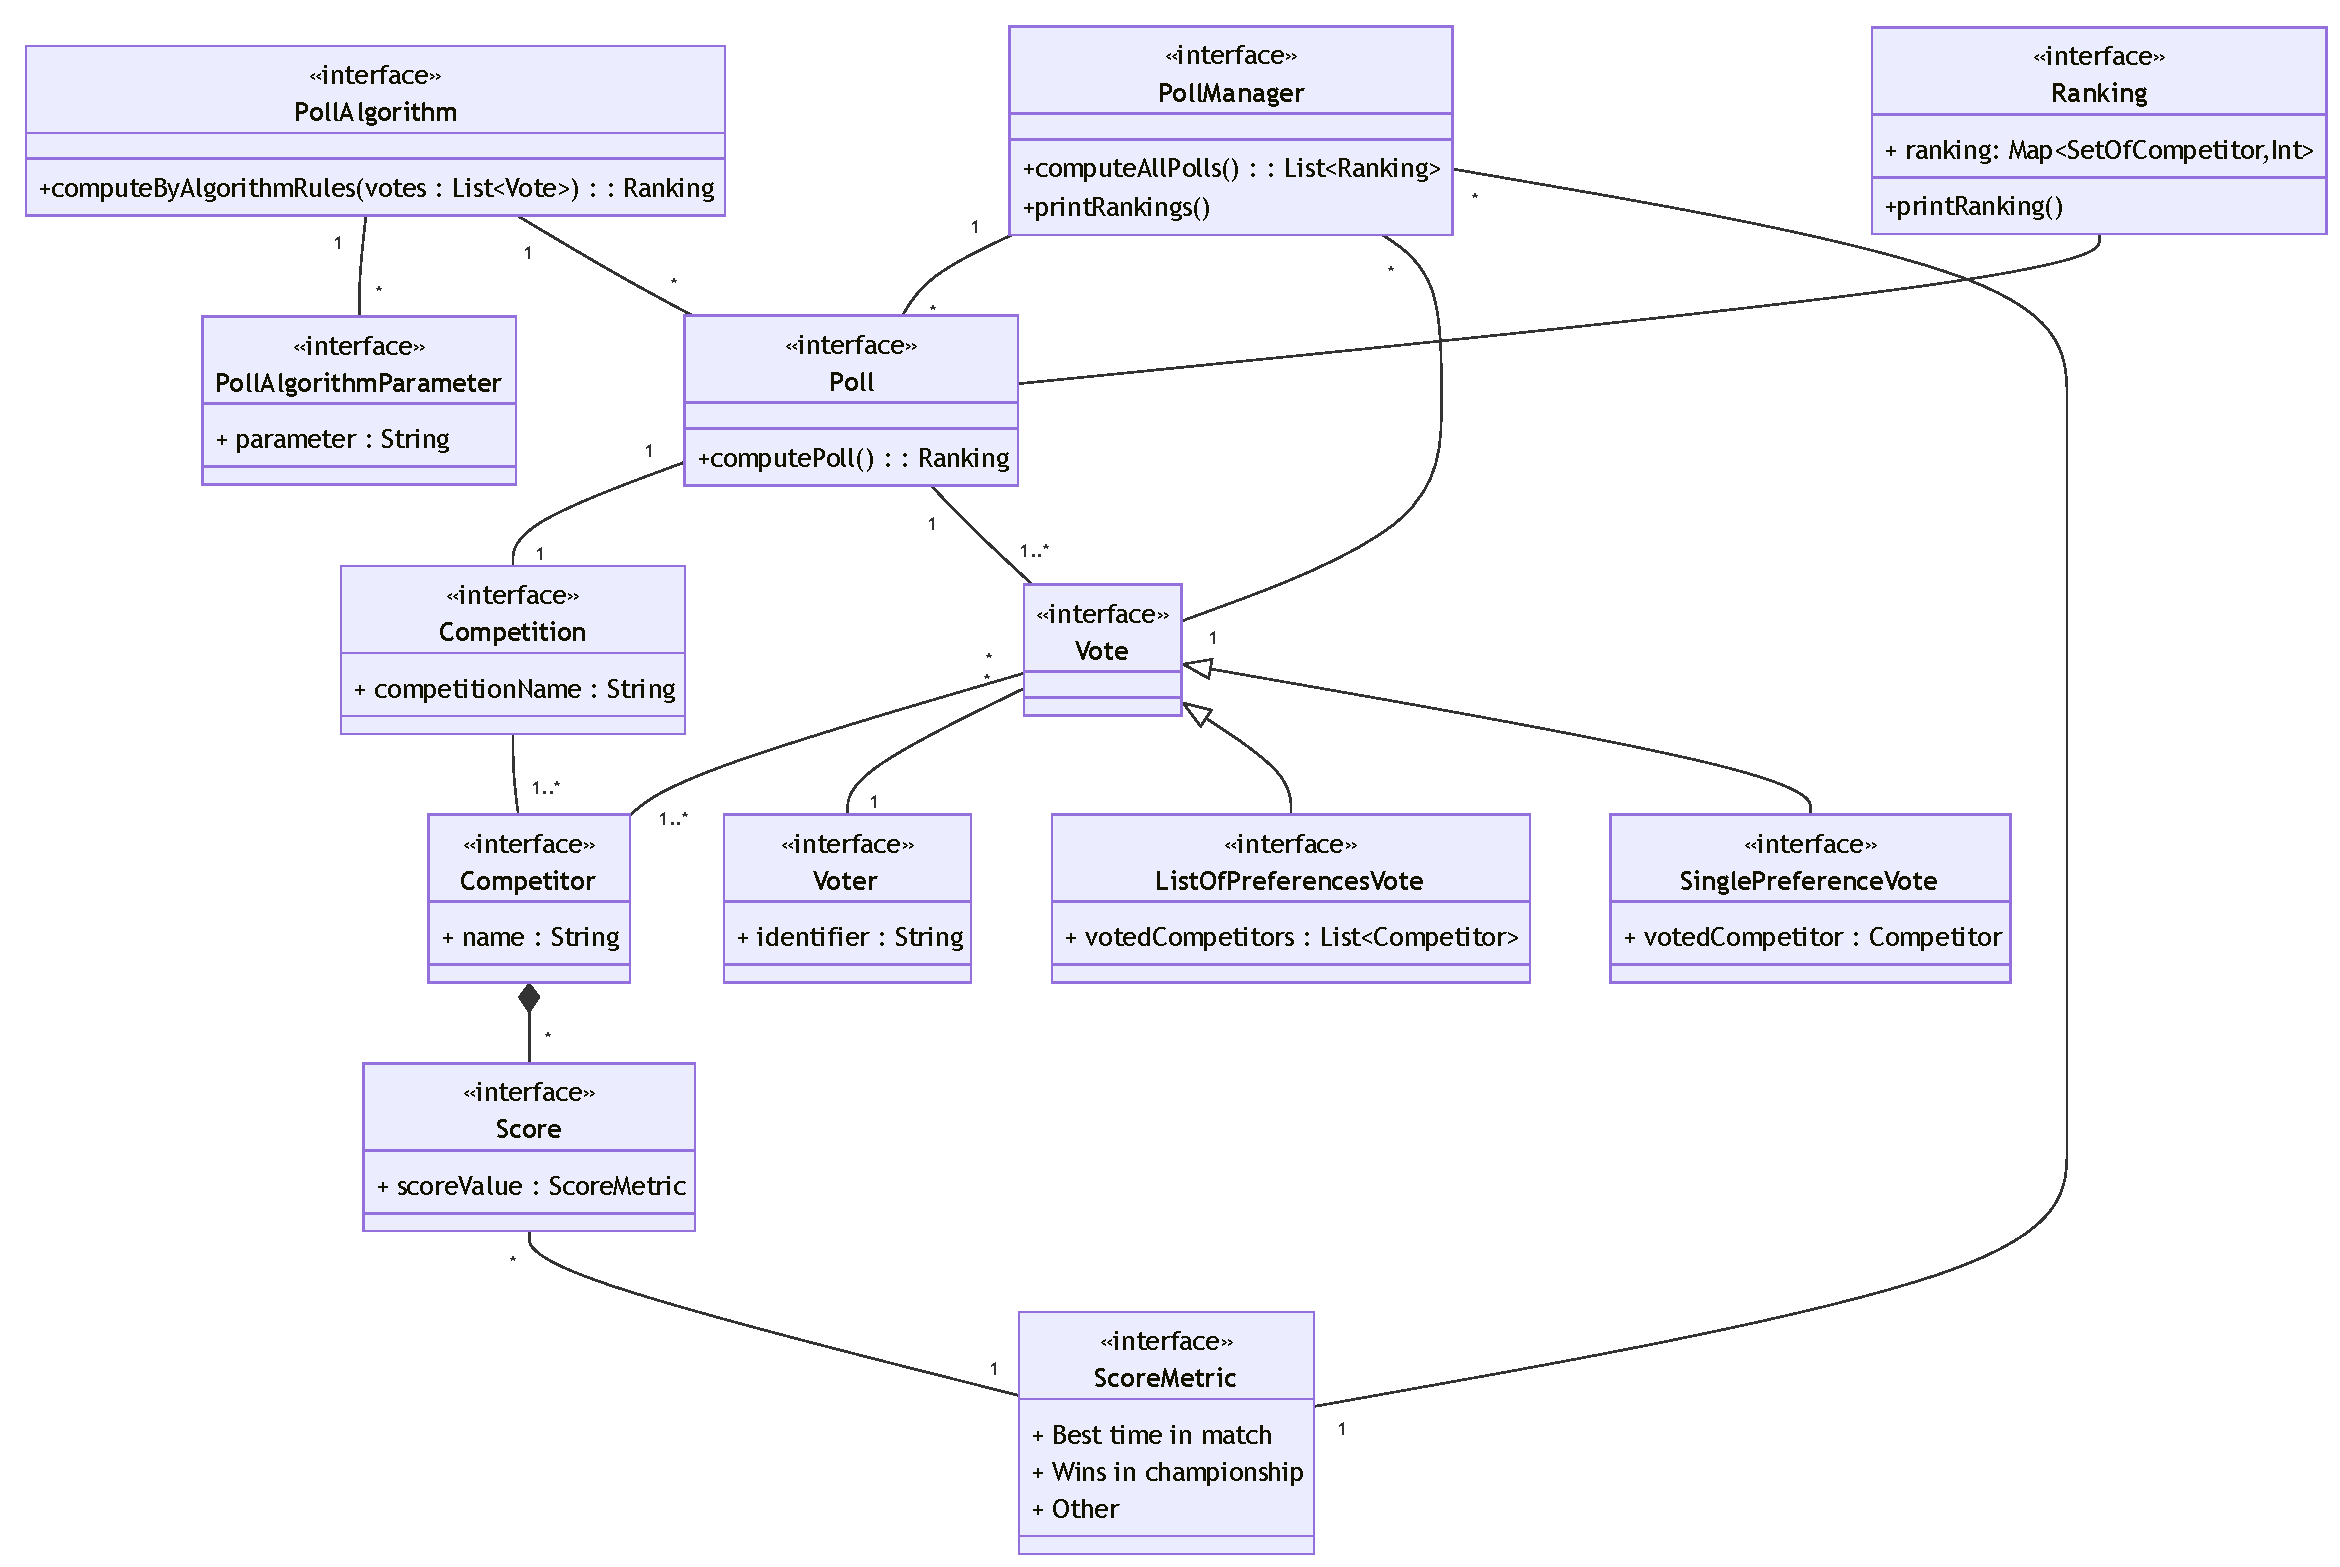
\includegraphics[width=1.2\linewidth, left]{figures/modellodominio.pdf}
    \caption{Diagramma UML del modello del dominio di EleKtion}
   \label{fig:modellodominio}
\end{figure}

%----------------------------------------------------------------------------------------
\chapter{Design}
\label{designdsl}
In questo capitolo, partendo dalla modellazione del dominio descritta nel paragrafo \ref{modellodominio}, 
viene sviluppato un approfondimento sulla definizione delle metriche di punteggio e sulla porzione
impattata dall'introduzione di \ac{dsl}, volto alla semplificazione dell'utilizzabilità della libreria EleKtion.
Ciascuna funzionalità viene approfondita in un apposito paragrafo, contenente un diagramma UML
che esplica l'organizzazione di interfacce e classi astratte.
Questi diagrammi sono realizzati con il presupposto di poter adottare l'utilizzo
dei seguenti costrutti:
\begin{itemize}
\item{\texttt{Tipi generici}\footnote{\url{https://archive.is/kISda}};}
\item{\texttt{Overloading} degli \texttt{operatori}\footnote{\url{https://archive.is/cExIS}};}
\item{\texttt{Higher order functions} (\texttt{function literal with receiver})\footnote{\url{https://archive.is/mWF2b}};}
\item{\texttt{Companion object}\footnote{\url{https://archive.is/yfHS5}}.}
\end{itemize}
Si rimanda alle fonti per l'approfondimento specifico in \texttt{Kotlin}, la sintassi utilizzata nei diagrammi
è generica ed astrae dal linguaggio specifico.
\section{Domain Specific Language per la definizione del gestore delle votazioni }
Questo \ac{dsl} è pensato per facilitare la creazione del gestore delle votazioni.
Il gestore delle votazioni adotta uno specifico tipo \texttt{S}, sottotipo di \texttt{ScoreMetric}, ed uno specifico
tipo di voto \texttt{V}, sottotipo di \texttt{Vote}.
Una metrica è definibile come il criterio tale per cui un concorrente può essere messo a confronto con un altro, sulla base della
sua prestazione nella competizione. Pertanto, è rappresentabile come una comparazione tra valori.
Dall'interfaccia \texttt{ScoreMetric} possono essere definiti numerosi sottotipi utili alla competizione trattata, ad esempio il punteggio di un concorrente
può essere legato ai punti assegnati in una gara, alle vittorie ottenute in campionato, oppure a criteri legati al tempo.
Per semplificarne la creazione è utile definire una funzione di supporto contenuta in un oggetto \texttt{companion}, come mostrato in figura \ref{fig:metrica}.

\vfill
\begin{center} 
\begin{figure}[H]
    \centering
     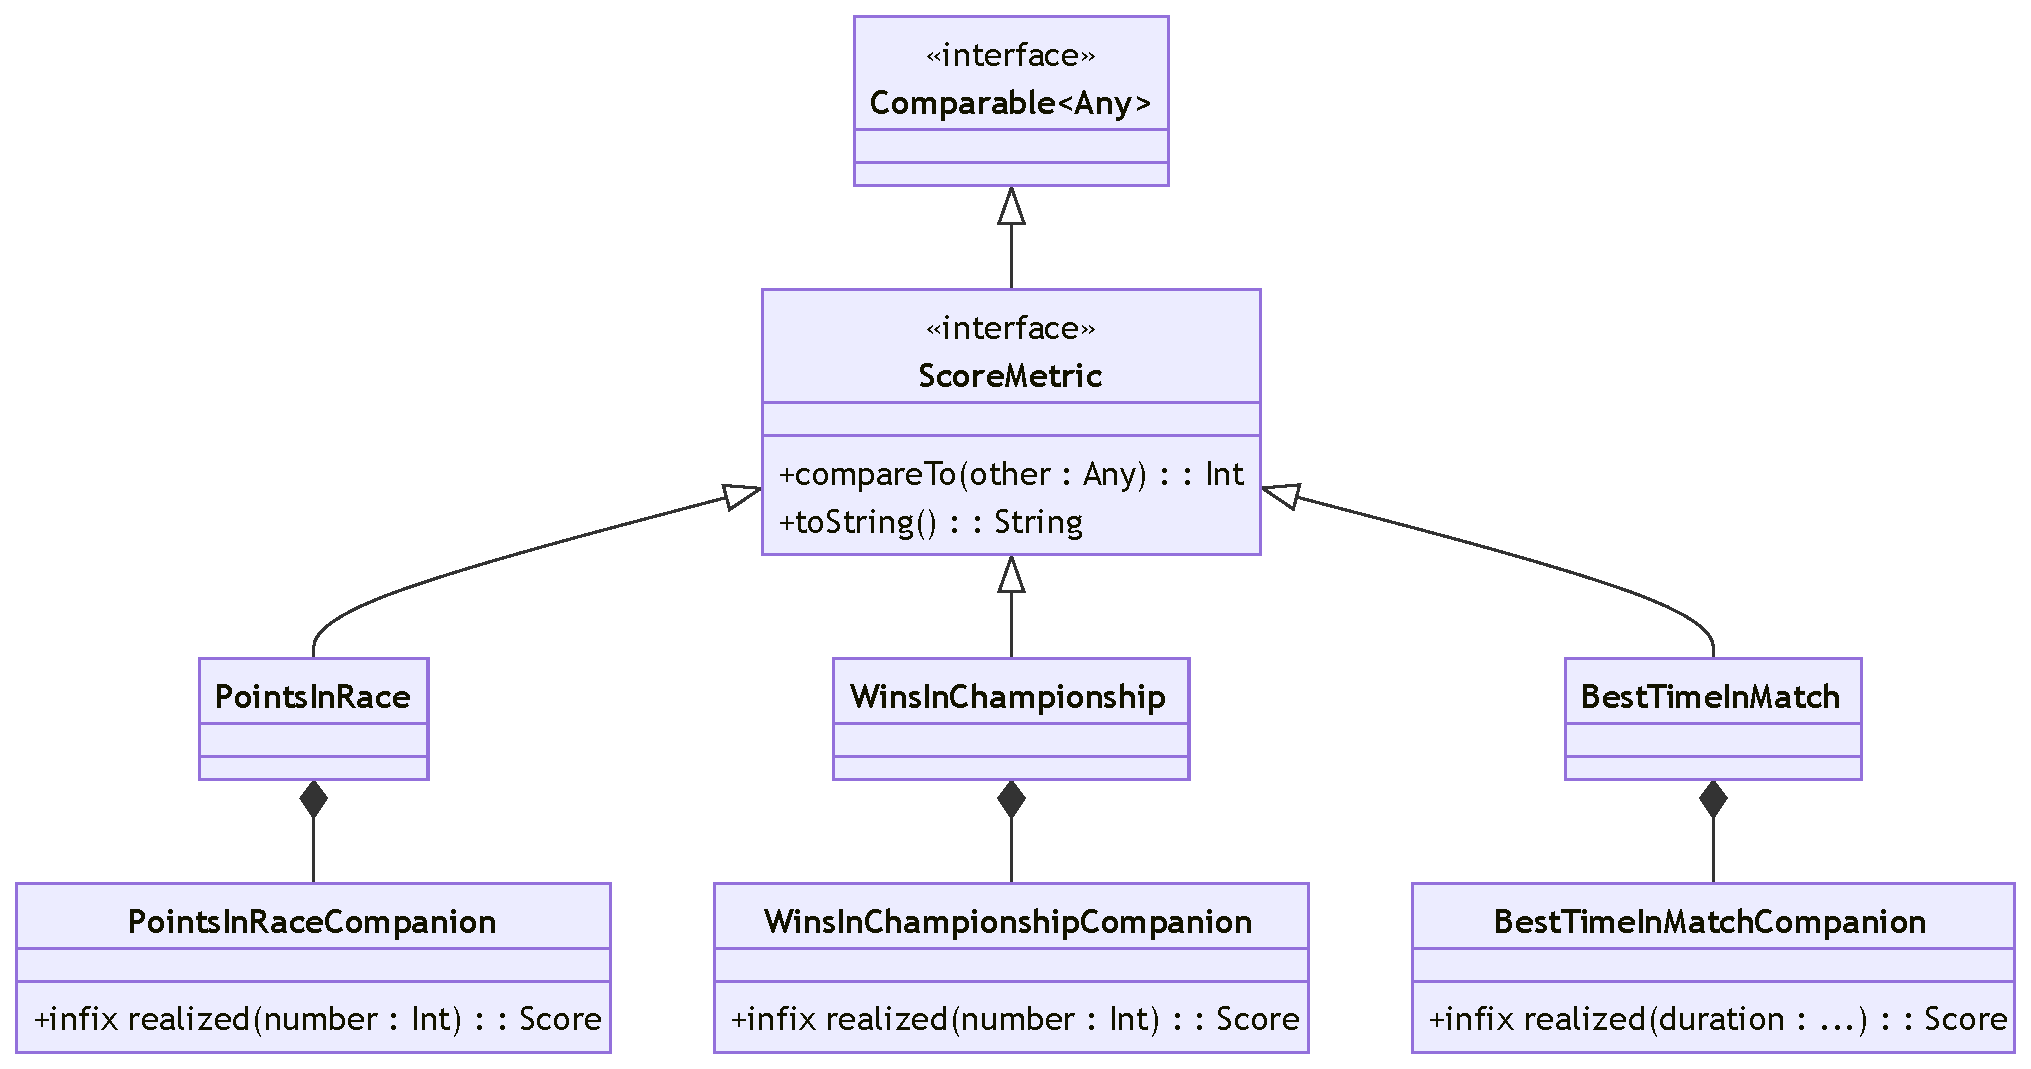
\includegraphics[width=1.1\linewidth]{figures/scoremetric.pdf}
     \caption{Diagramma UML dell'organizzazione di una metrica}
    \label{fig:metrica}
 \end{figure}
\end{center}
\vfill

I tipi \texttt{S} e \texttt{V} vincolano i seguenti componenti che verranno trattati, pertanto non è possibile adottare diverse metriche di punteggio
o diverse tipologie di voto tra le varie votazioni presenti nel medesimo gestore.
Il punto di ingresso dell'intero flusso è rappresentato dalla funzione \texttt{initializedAs}, al suo interno è possibile inizializzare una votazione attraverso 
la funzione \texttt{poll}, e l'utilizzo dell'operatore unario \texttt{+}, per l'aggiunta di quest'ultima alla lista delle votazioni.
In figura \ref{fig:pollManagerDSL} viene mostrato il diagramma UML delle interfacce e della classe astratta.
\vfill
\begin{center} 
\begin{figure}[H]
    \centering
     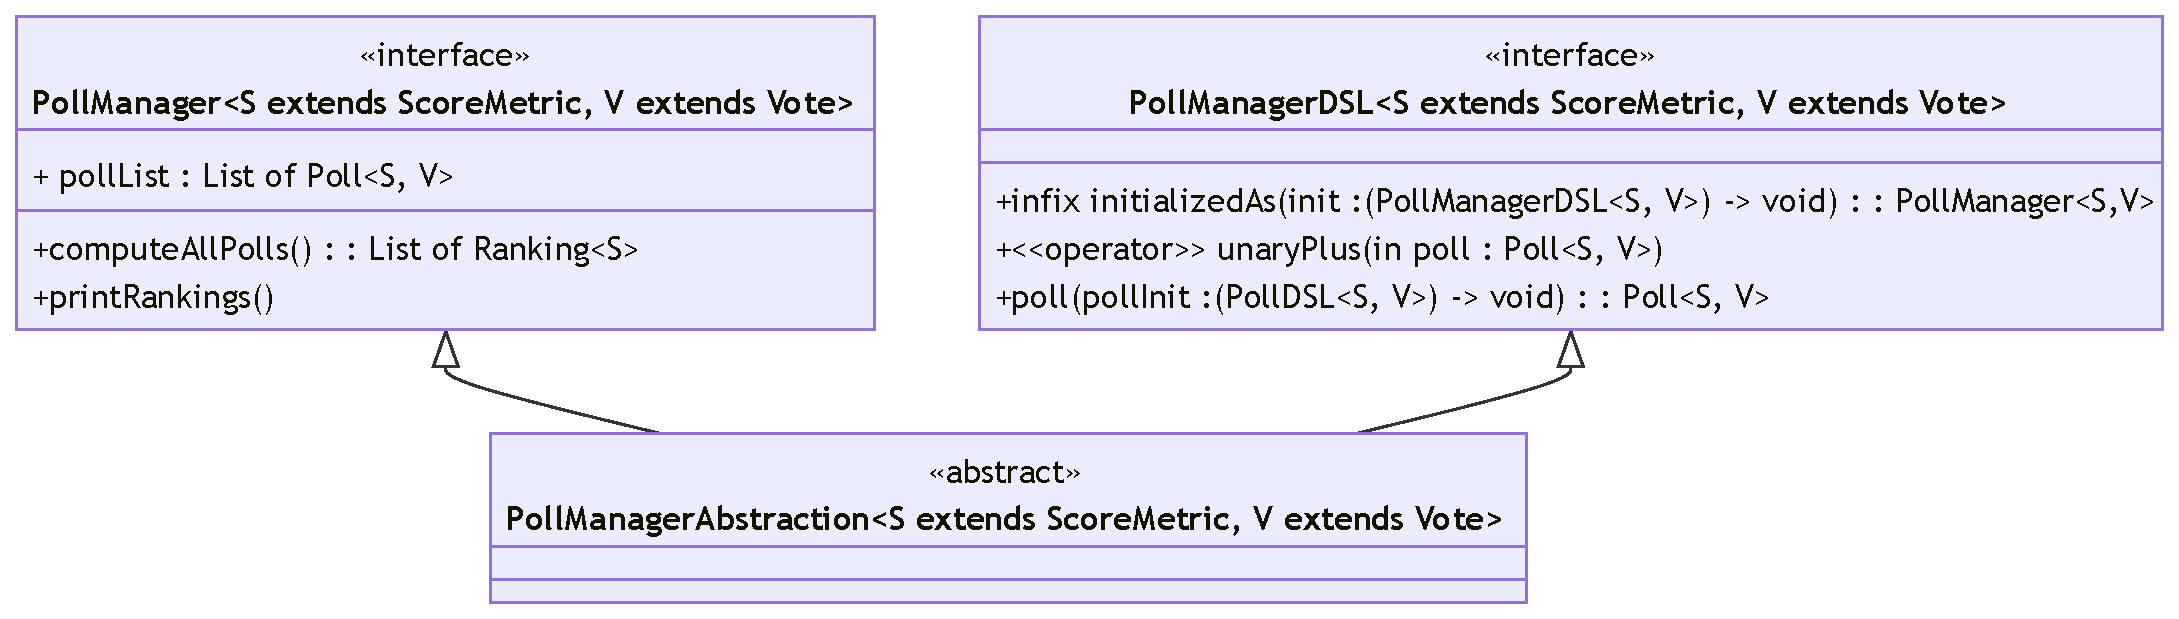
\includegraphics[width=1.1\linewidth]{figures/pollManagerDSL.pdf}
     \caption{Diagramma UML del \ac{dsl} per la definizione del gestore delle votazioni}
    \label{fig:pollManagerDSL}
 \end{figure}
\end{center}
\vfill
 \newpage
 \section{Domain Specific Language per la definizione della votazione}
 Questo \ac{dsl} è pensato per facilitare la creazione di una votazione.
 In base al tipo di voto viene definito un costrutto per agevolarne la creazione.
 Nel caso in cui il voto sia a singola preferenza, è necessario specificare
 l'identificativo del votato e l'identificativo del votante (vedi funzione \texttt{votedBy} in \texttt{SinglePreferenceVoteAlgorithmDSL}, figura \ref{fig:SPPollAlgorithmDSL}). Se quest'ultimo non 
 deve essere pubblico, corrisponderà ad un identificativo casuale (vedi funzione \texttt{asAnonymousVote} in \texttt{SinglePreferenceVoteAlgorithmDSL}, figura \ref{fig:SPPollAlgorithmDSL}).
 Nel caso in cui il voto sia a lista di preferenze, per costruire la lista è necessario specificare l'elenco degli identificativi dei votati,
 utilizzando la funzione \texttt{then} in concatenazione (vedi funzione \texttt{then} in \texttt{ListOfPreferencesVoteAlgorithmDSL}, figura \ref{fig:LOPPollAlgorithmDSL}).
 Allo stesso modo del voto a singola preferenza, è prevista la possibilità di anonimizzare il votante.
 Sono previsti metodi per semplificare l'inizializzazione degli algoritmi disponibili:
 \begin{itemize}
    \item{\texttt{majorityVotesAlgorithm}: rappresenta la creazione di un algoritmo a maggioranza, in cui il vincitore è colui che ricevuto più voti;}
    \item{\texttt{majorityVotesHScoreAlgorithm}: rappresenta la creazione di un algoritmo a maggioranza, in cui il vincitore è colui che ricevuto più voti.
    Se si verificano pareggi, viene selezionato il concorrente che ha il punteggio maggiore, secondo la metrica di punteggio definita;}
    \item{\texttt{majorityVotesLScoreAlgorithm}: rappresenta la creazione di un algoritmo a maggioranza, in cui il vincitore è colui che ricevuto più voti.
    Se si verificano pareggi, viene selezionato il concorrente che ha il punteggio minore, secondo la metrica di punteggio definita;}
    \item{\texttt{condorcetAlgorithm}: rappresenta la creazione dell'algoritmo di Condorcet;}
    \item{\texttt{schultzeAlgorithm}: rappresenta la creazione dell'algoritmo di Schultze.}
 \end{itemize}
I parametri utili al funzionamento dell'algoritmo possono essere impostati utilizzando l'
operatore unario \texttt{+} presente in \texttt{PollAlgorithmDSL}.
In figura \ref{fig:pollDSL} vengono mostrati gli altri metodi utili alla creazione di una votazione:
la funzione \texttt{competition} istanzia una competizione,
richiedendo che vengano definiti il nome della competizione ed un inizializzatore in cui saranno specificati i candidati presenti.
La competizione, così come l'algoritmo scelto, sono effettivamente assegnati alla votazione
attraverso l'uso dell'operatore unario \texttt{-}.
Infine è possibile aggiungere un elenco di voti, istanziati utilizzando i metodi descritti nella prima parte
di questo paragrafo. Ciascun voto viene effettivamente aggiunto alla lista di voti attraverso
l'uso dell' operatore unario \texttt{+}.
Per motivi di spazio, nelle figure \ref{fig:SPPollAlgorithmDSL} e \ref{fig:LOPPollAlgorithmDSL} sono stati utilizzati gli
acronimi \texttt{SP} e \texttt{LOP}, al posto di, rispettivamente, \texttt{SinglePreference} e \texttt{ListOfPreferences}.

 \vfill
 \begin{center} 
 \begin{figure}[H]
     \centering
      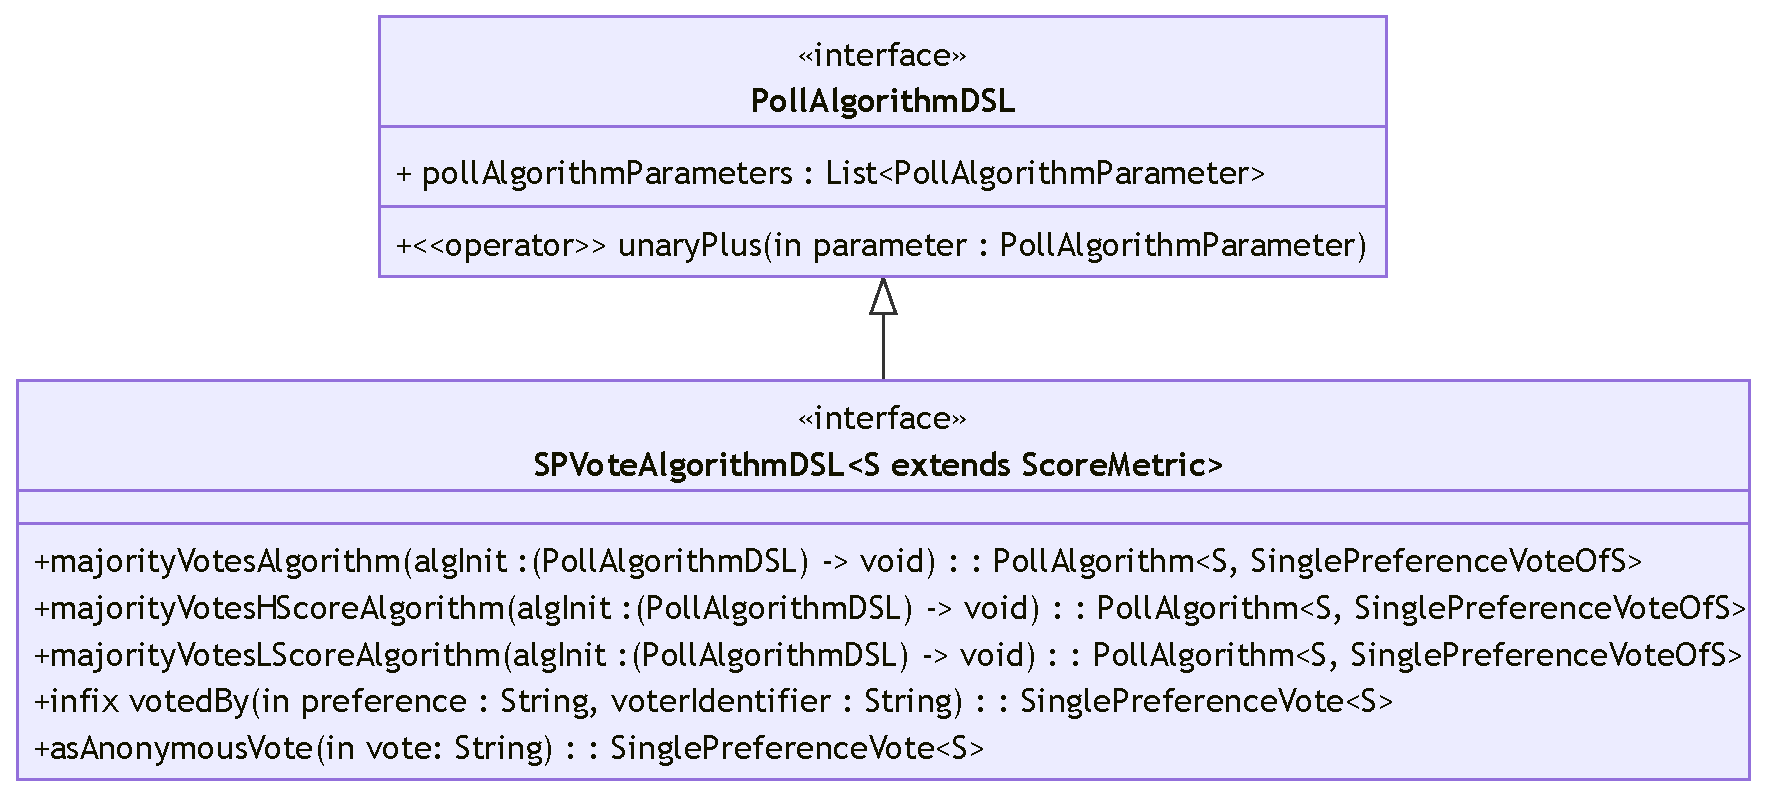
\includegraphics[width=1.1\linewidth]{figures/SPPollAlgorithmDSL.pdf}
      \caption{Diagramma UML del \ac{dsl} per la definizione dell'algoritmo a singola preferenza}
     \label{fig:SPPollAlgorithmDSL}
  \end{figure}
\end{center}
\vfill

\vfill
\begin{center} 
\begin{figure}[H]
    \centering
     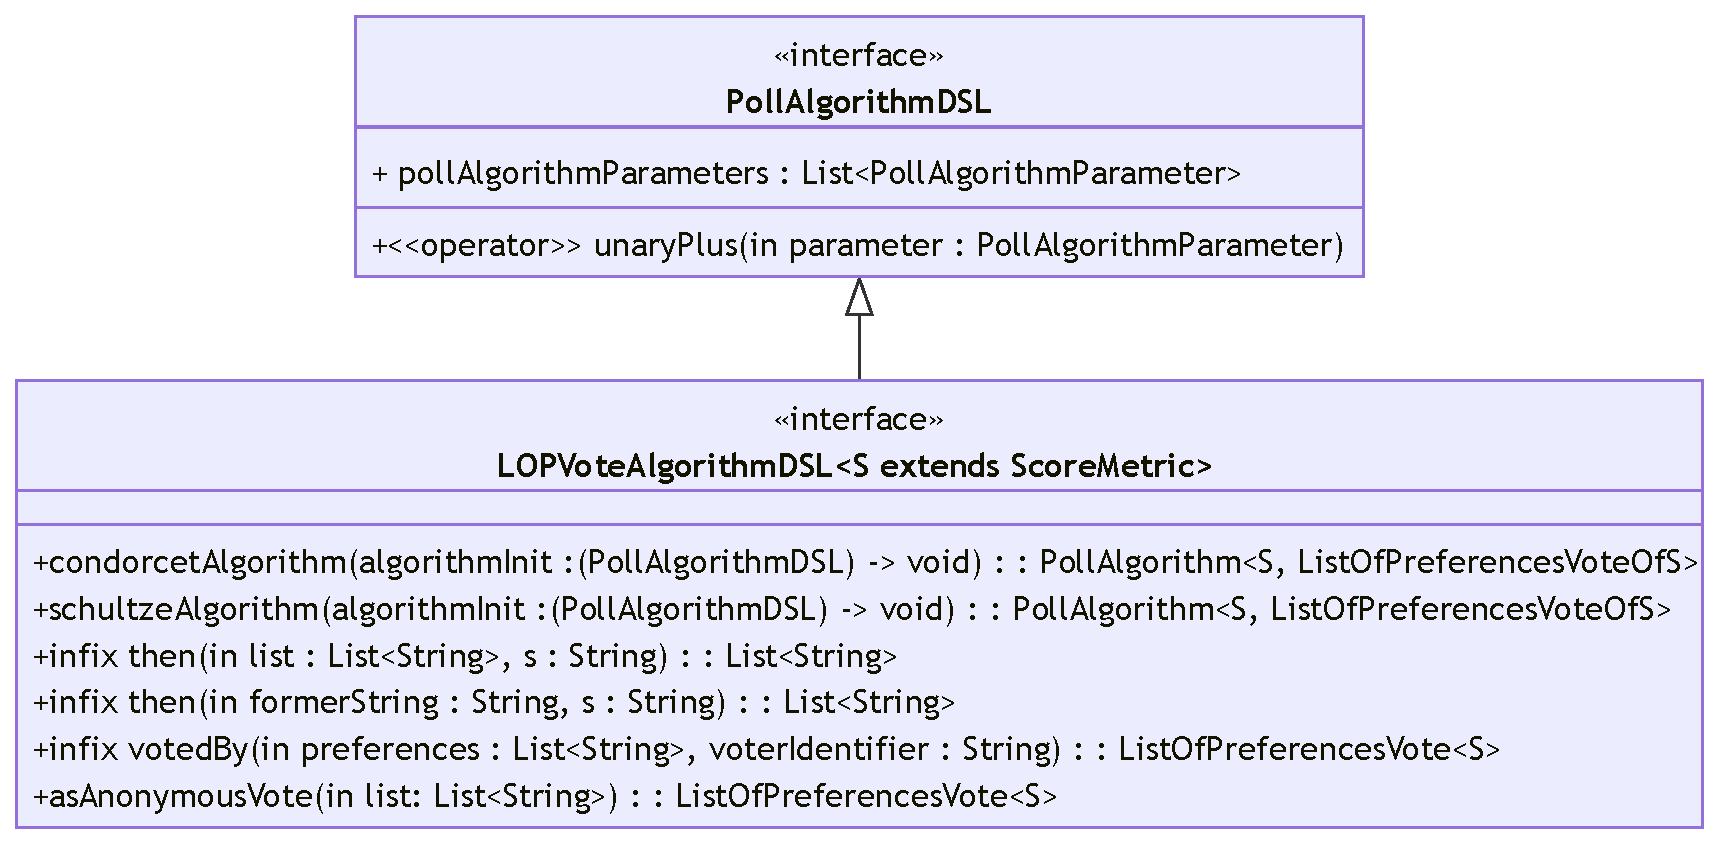
\includegraphics[width=1.1\linewidth]{figures/LOPPollAlgorithmDSL.pdf}
     \caption{Diagramma UML del \ac{dsl} per la definizione dell'algoritmo a lista di preferenze}
    \label{fig:LOPPollAlgorithmDSL}
 \end{figure}
\end{center}
\vfill



\vfill
\begin{center}
 \begin{figure}[H]
     \centering
      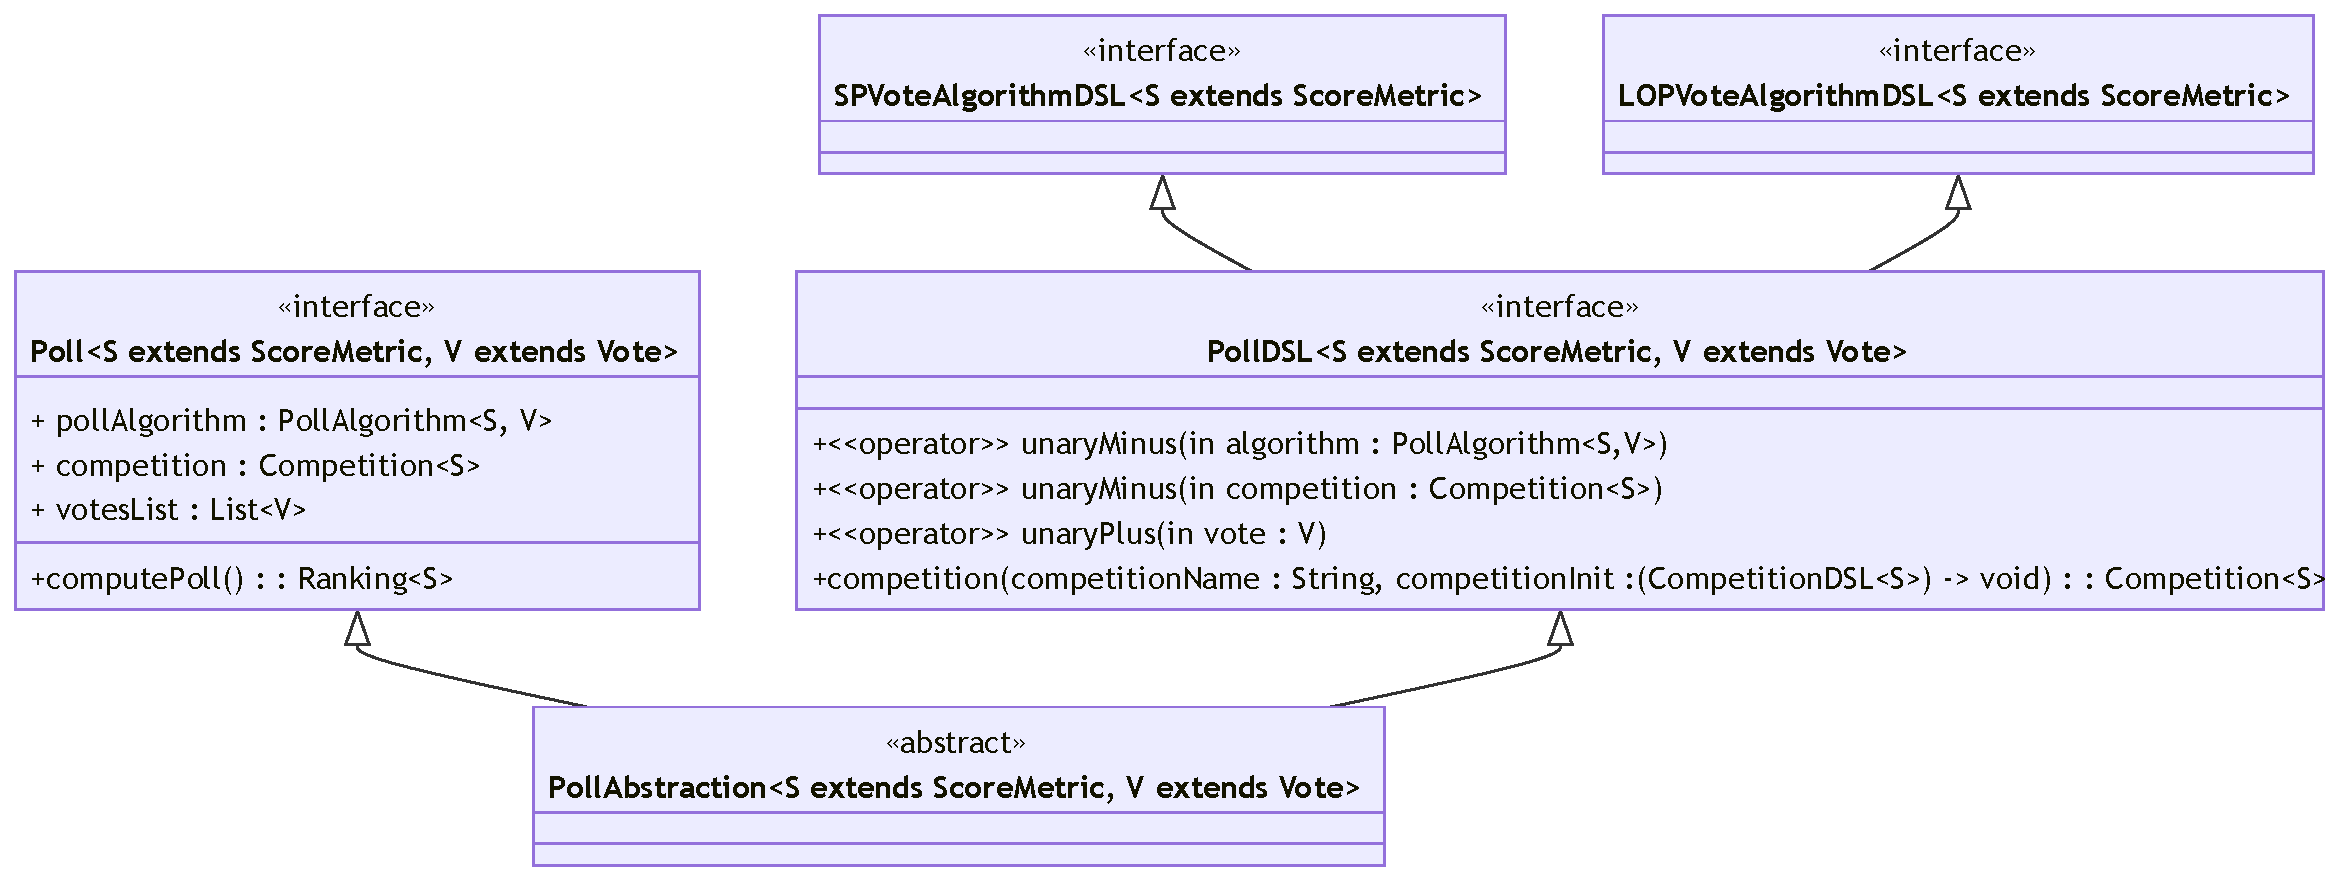
\includegraphics[width=1.1\linewidth]{figures/pollDSL.pdf}
      \caption{Diagramma UML del \ac{dsl} per la definizione della votazione}
     \label{fig:pollDSL}
  \end{figure}
\end{center}
\vfill
  



\section{Domain Specific Language per la definizione della competizione}
\label{dslcompetizione}
Questo DSL è pensato per facilitare la creazione ed il popolamento di una competizione.
La funzione \texttt{competitor} istanzia un concorrente,
richiedendo che sia specificato il proprio identificativo ed un inizializzatore contenente i punteggi realizzati.
Il concorrente istanziato, viene aggiunto alla lista dei concorrenti grazie all'uso dell'operatore unario \texttt{+} .
In figura \ref{fig:competitionDSL} viene mostrato il diagramma UML delle interfacce e della classe astratta.
\begin{figure}[H]
    \centering
     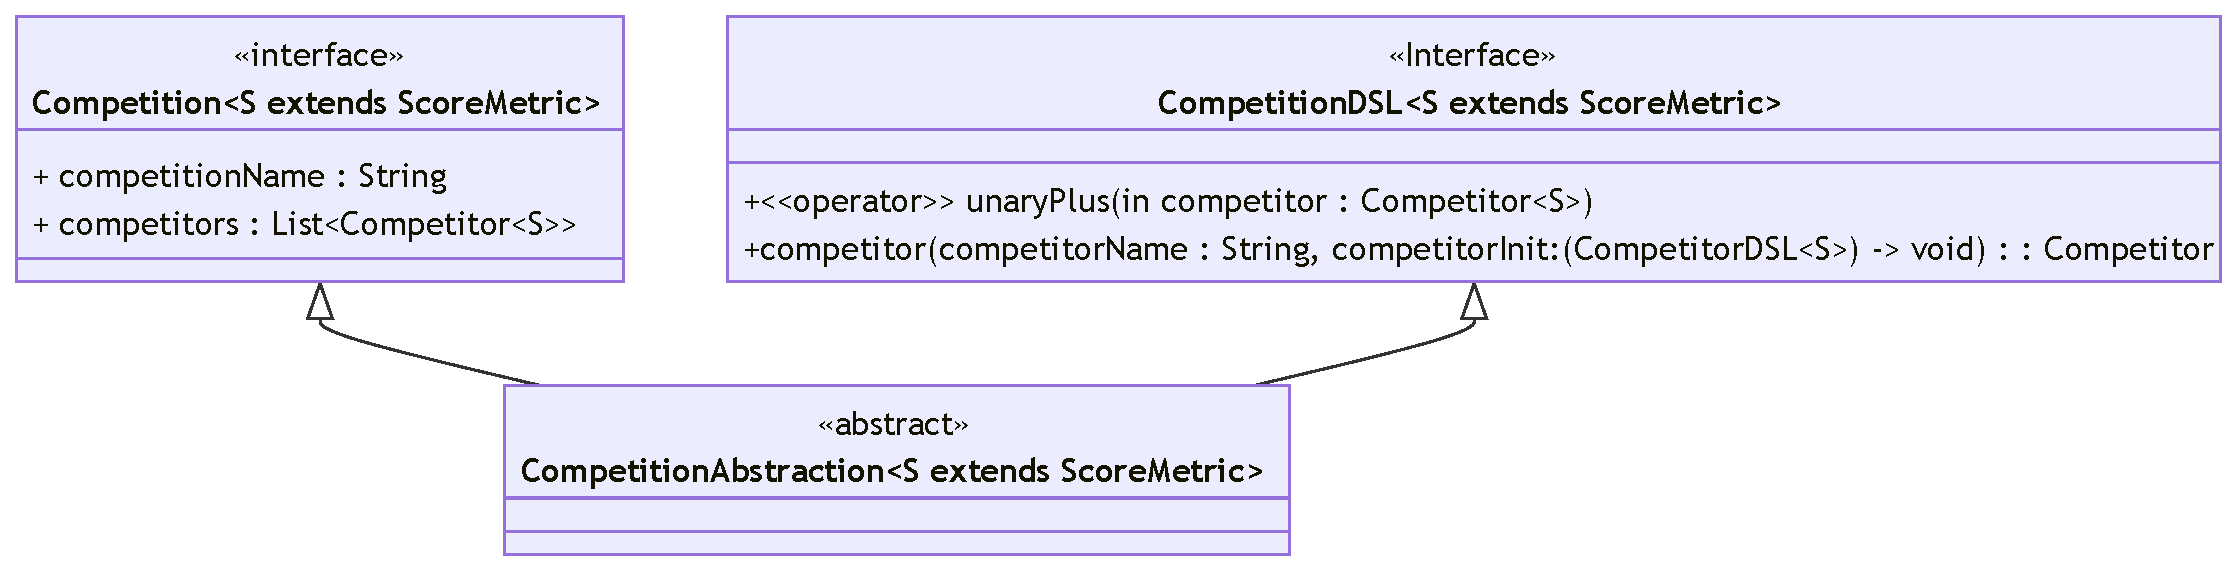
\includegraphics[width=1.1\linewidth]{figures/competitionDSL.pdf}
     \caption{Diagramma UML del \ac{dsl} per la definizione della competizione}
    \label{fig:competitionDSL}
 \end{figure}
 \newpage

\section{Domain Specific Language per la definizione del concorrente}
Questo DSL è ideato per facilitare la creazione di un concorrente.
Ciascun concorrente può avere un elenco di punteggi, i quali vengono
assegnati attraverso l'uso dell'operatore unario \texttt{+}.
\begin{figure}[H]
    \centering
     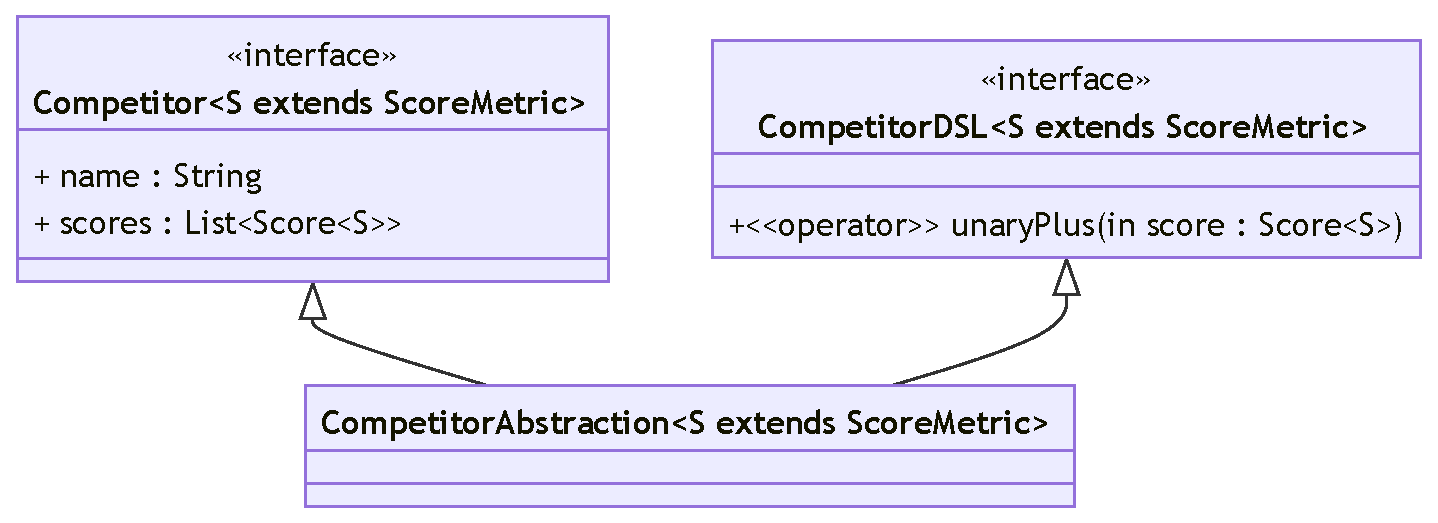
\includegraphics[width=1.1\linewidth]{figures/competitorDSL.pdf}
     \caption{Diagramma UML del \ac{dsl} per la definizione del concorrente}
    \label{fig:competitorDSL}
 \end{figure}
 \newpage

%----------------------------------------------------------------------------------------
\chapter{Implementazione}
In questo capitolo vengono mostrati alcuni casi d'uso realizzati per verificare il corretto funzionamento della libreria,
dando nota delle possibili eccezioni che sono state gestite.
Successivamente, viene fornita una panoramica sul processo di \textit{build automation} e
vengono mostrati gli step realizzati per volgere alla creazione e pubblicazione della libreria.
Per la libreria, il cui codice sorgente è reperibile all'indirizzo https://github.com/corinz97/EleKtion, \\
sono stati adottati \texttt{Kotlin} come linguaggio di programmazione
e \texttt{Gradle} come tool a supporto della \textit{build automation}.
\section{Casi realizzati per i differenti tipi di algoritmo}
Nel paragrafo \ref{modellodominio} e nel capitolo \ref{designdsl} è stata presentata l'organizzazione del dominio
da implementare, assieme ad un approfondimento sulle entità che compongono il linguaggio \ac{dsl}
ideato appositamente per questa libreria.
In questo capitolo vengono mostrati alcuni dei casi d'uso che sono stati realizzati per verificare il corretto funzionamento della libreria,
spiegando come vengono gestiti eventuali conflitti a seconda dell'algoritmo scelto.
\subsection{Votazioni a singola preferenza}
Per gestire le votazioni a singola preferenza è stato creato inizialmente il caso base per la votazione a maggioranza,
nella quale il vincitore è il concorrente che riceve più voti, a prescindere dalla presenza di altri criteri come i punteggi.
In alcuni casi è possibile avere parità tra i voti, appaiono più vincitori nella stessa posizione. 
Successivamente è stata estesa la gestione dei pareggi, dando la possibilità all'utilizzatore della libreria di definire 
una metrica per la competizione ed un elenco di punteggi realizzati da ciascun concorrente, basati su quella metrica.
Nel caso in cui si ha un pareggio di voti è possibile decidere di effettuare un ulteriore sotto-confronto basato sui punteggi,
per selezionare chi risulta vincitore sulla base del punteggio più basso o più alto realizzato nella competizione.
Questo sotto-confronto può portare ad avere dei vincitori a pari merito, oppure di piazzarli in posizioni differenti, proprio
per la differenza dei punteggi.
La gestione quindi non garantisce l'assenza totale di pareggi, che può verificarsi anche a livello di punteggio.
Inoltre, è possibile avere un parametro che indica la capacità di effettuare molteplici voti per votante, ma di negargli
comunque l'opportunità di votare più volte lo stesso candidato.
Le classi realizzate per gestire tutte queste casistiche sono \texttt{MajorityVotesAlgorithm}, \texttt{MajorityVotesThenHighestScoreAlgorithm}
e \texttt{MajorityVotesThenLowestScoreAlgorithm}. Nell'estratto di codice \ref{lst:controllisinglevote} vengono mostrati i controlli effettuati prima di 
compiere la scelta del vincitore.
\lstinputlisting[language=Kotlin,label={lst:controllisinglevote}, caption={Controlli effettuati prima di compiere la scelta del vincitore, nella votazione a singola preferenza}]{listings/controlliSingleVote.kt}
Successivamente, viene generata la classifica, che contiene l'insieme dei vincitori con il relativo numero di voti. Per ciascun vincitore,
viene riportato il punteggio maggiore o quello minore. Nel caso in cui si utilizzi l'algoritmo a maggioranza senza sotto-confronto, vengono riportati
tutti i punteggi realizzati, inoltre per quest'ultimo non è obbligatorio associare dei punteggi ai giocatori.
Negli estratti di codice \ref{lst:esempiosinglevotemajority}, \ref{lst:esempiosinglevotemajorityhighestscore} e \ref{lst:esempiosinglevotemajoritylowestscore}  vengono mostrati alcuni esempi realizzati: nella definizione di ogni competizione
è essenziale dichiarare l'elenco di tutti i possibili candidati in modo da poter verificare che non ci siano voti associati ad un candidato non esistente.
Questo controllo è effettuato anche dal DSL nella fase di definizione dei voti, e quindi in precedenza all'invocazione dell'algoritmo,
il quale replica questo controllo in quanto è possibile utilizzarlo indipendentemente dall'adozione di DSL.
Si definisce poi l'algoritmo da utilizzare e l'elenco di voti. I voti possono essere anonimizzati, generando una stringa \texttt{UUID} che viene usata come identificativo del votante.
\lstinputlisting[language=Kotlin,label={lst:esempiosinglevotemajority}, caption={Votazione a singola preferenza, in cui il vincitore è competitor1. }]{listings/esempioSingleVoteMajority.kt}
\lstinputlisting[language=Kotlin,label={lst:esempiosinglevotemajorityhighestscore}, caption={Votazione a singola preferenza, in cui il vincitore è competitor1. }]{listings/esempioSingleVoteMajorityHighestScore.kt}
\lstinputlisting[language=Kotlin,label={lst:esempiosinglevotemajoritylowestscore}, caption={Votazione a singola preferenza, in cui competitor1 e competitor2 pareggiano.}]{listings/esempioSingleVoteMajorityLowestScore.kt}
Sono stati realizzati test a supporto dell'utilizzo del DSL e degli algoritmi, in particolare è stato verificato che venga 
restituita un' eccezione nei casi in cui: 
\begin{enumerate}
    \item{Nell'ambito degli algoritmi, in una determinata votazione
        \begin{itemize}
        \item{un candidato sia presente più di una volta nell'insieme dei candidati;}
        \item{non siano presenti voti;}
        \item{un votante effettui più di un voto, a meno di passare all'algoritmo l'apposito parametro;}
        \item{il parametro, quando presente, sia dichiarato più di una volta;}
        \item{un votante voti due volte lo stesso candidato, seppur in presenza del parametro;}
        \item{un votante voti un candidato non esistente;}
        \item{la classifica generata non contenga alcun elemento;}
        \item{la classifica generata restituisca i risultati ordinati in modo non decrescente di voti;}
        \item{gli algoritmi che utilizzano il sotto-criterio rilevino che ci sono concorrenti senza alcun punteggio.}
        \end{itemize}}
    \item{Nell'ambito del DSL
        \begin{itemize}
            \item{non siano presenti voti;}
            \item{si dichiari lo stesso candidato più di una volta nell'insieme di candidati;}
            \item{si dichiari un voto per un candidato non esistente}
        \end{itemize}
    }

\end{enumerate}

\subsection{Votazioni a lista di preferenze}
Per gestire la votazioni a lista di preferenze è stato necessario procedere all'implementazione dell'algoritmo di
Condorcet e dell'algoritmo di Schultze. Come è stato descritto in \ref{chapter:votazionilistapreferenze}, quest'ultimo
è una variante del primo, pertanto condividono buona parte della logica.
Inizialmente usando una matrice di dimensione \textit{n x n}, dove \textit{n} è il numero dei candidati, ed esaminando l'indice in cui si posizionano i 
candidati in un voto, si evidenzia chi dei due abbiamo ottenuto un punto. Si ottiene quindi una matrice che indica quante volte 
sono stati vinti gli scontri di coppia tra due determinati candidati.
Successivamente, l'algoritmo di Condorcet effettua tante iterazioni quanti sono i concorrenti rimasti da piazzare in graduatoria,
ed in ogni iterazione si esamina quali siano i candidati che hanno battuto tutti gli altri nello scontro a coppie.
Anche l'algoritmo di Schultze effettua tante iterazioni quanti sono i concorrenti rimasti da piazzare in graduatoria, ed in ogni iterazione
si determinano quali sono i candidati che hanno ottenuto il maggior numero di vittorie negli scontri a coppie.
Pertanto, è stata ammessa la possibilità di ottenere dei pareggi a parità di posizionamento.
Anche per questa tipologia di votazione è possibile avere un parametro che indica la capacità di effettuare molteplici voti per votante , ma di negargli
comunque l'opportunità di votare più volte lo stesso candidato.
Le classi realizzate per gestire le casistiche sono \texttt{CondorcetAlgorithm} e \\
\texttt{SchultzeAlgorithm}.
Nell'estratto di codice \ref{lst:controllilopvote} vengono mostrati i controlli effettuati prima di 
eseguire l'algoritmo di votazione.
\lstinputlisting[language=Kotlin,label={lst:controllilopvote}, caption={Controlli effettuati prima della votazione a lista di preferenze}]{listings/controlliLOPVote.kt}
Infine viene generata la classifica contenente l'elenco dei vincitori, posti in ordine di preferenza decrescente secondo la logica dell'algoritmo selezionato.
A parità di posizione è possibile trovare
più di un candidato e non è previsto riportare il numero di voti, poichè è scollegato dalla logica algoritmica.
Negli estratti di codice \ref{lst:esempiolopvotecondorcet} e \ref{lst:esempiolopvoteschultze} vengono mostrati alcuni esempi realizzati: nella definizione di ogni competizione
è essenziale dichiarare l'elenco di tutti i possibili candidati in modo da poter verificare che non ci siano voti associati ad un candidato non esistente.
Questo controllo è effettuato anche dal DSL nella fase di definizione dei voti, e quindi in precedenza all'invocazione dell'algoritmo,
che replica questo controllo in quanto è possibile utilizzarlo indipendentemente dall'adozione di DSL.
Si definisce poi l'algoritmo da utilizzare e l'elenco di voti. 
I voti possono essere anonimizzati, come nel caso delle votazioni a preferenza singola.
\lstinputlisting[language=Kotlin,label={lst:esempiolopvotecondorcet}, caption={Votazione a lista di preferenze con l'algoritmo di Condorcet, in cui la classifica generata è competitorC, competitorA, competitorB}]{listings/esempioLOPVoteCondorcet.kt}
\lstinputlisting[language=Kotlin,label={lst:esempiolopvoteschultze}, caption={Votazione a lista di preferenze con l'algoritmo di Schultze, in cui la classifica generata è competitorC, competitorA, competitorB}]{listings/esempioLOPVoteSchultze.kt}
Sono stati realizzati test a supporto dell'utilizzo del DSL e degli algoritmi, in particolare è stato verificato che venga 
restituita un' eccezione nei casi in cui: 
\begin{enumerate}
    \item{Nell'ambito degli algoritmi, in una determinata votazione
        \begin{itemize}
        \item{un candidato sia presente più di una volta nell'insieme dei candidati;}
        \item{un votante effettui più di un voto, a meno di passare all'algoritmo l'apposito parametro;}
        \item{il parametro, quando presente, sia dichiarato più di una volta;}
        \item{un votante voti due volte la stessa lista, seppur in presenza del parametro;}
        \item{un votante voti una lista in cui appaia un candidato non esistente;}
        \item{un votante voti una lista in cui sia stato omesso almeno un candidato;}
        \item{un votante voti una lista in cui un candidato appaia più volte;}
        \item{non siano presenti voti;}
        \item{la classifica generata non contenga alcun elemento.}
       \end{itemize}}
    \item{Nell'ambito del DSL
        \begin{itemize}
            \item{si dichiari un candidato più di una volta nell'insieme di candidati;}
            \item{si dichiari un voto per un candidato non esistente;}
            \item{si dichiari un voto in cui un candidato appaia più volte;}
            \item{non siano presenti voti.}
        \end{itemize}
    }

\end{enumerate}
Utilizzando il DSL, è possibile dichiarare voti in cui non appaiono tutti i possibili candidati e in tal caso,
questi saranno piazzati in fondo alla lista, ossia come più sfavoriti.
\section{Build automation}
L'adozione di un sistema di \textit{build automation} è un fattore chiave per la produzione
efficace ed efficiente di software di qualità.
Come principio base, è importante che ciascuna modifica apportata al codice
sia testata a livello unitario e abbia documentazione correlata, che sia la pubblicazione 
di una nuova funzionalità piuttosto che la variazione di un campo, a titolo meramente
esemplificativo. 
Inoltre, queste modifiche devono essere ulteriormente 
verificate attraverso test di integrazione, in modo da garantire la piena
compatibilità con i componenti pre-esistenti. 
Le verifiche possono essere effettuate 
manualmente dallo sviluppatore, ma per ridurre il rischio di errori è
possibile adottare un sistema di automazione, che attraverso una serie di task predefiniti
e ripetibili, verifichi automaticamente gli step,
gestendo anche le dipendenze tra gli stessi.
Così facendo, si può subito notare se tutto è andato a buon fine oppure 
se è necessario effettuare ulteriori eventi correttivi.
Una volta che il flusso di compilazione e verifica viene terminato con successo,
è possibile procedere alla generazione di uno o più artefatti e della relativa documentazione.
Questi prodotti possono essere sottoposti ad un operazione di versionamento,
in modo da distinguere le evoluzioni del software e semplificarne la distribuzione
e la tracciabilità.
Poichè gli artefatti generati sono dipendenti dall'architettura della macchina
e dal sistema operativo sui quali avviene il processo di \textit{build}, è opportuno eseguirlo
su piattorme dedicate come \ac{gh}.
\ac{gh} fornisce ambienti standard e personalizzabili
in base a direttive, gestendo il processo di \ac{ci}/\ac{cd} che è stato descritto in questo paragrafo. 
Infine, per favorire la distribuzione e la compatibilità verso molteplici sistemi,
è utile adottare strumenti come \texttt{Kotlin Multiplatform},
che semplificano la generazione dell'output finale adattandolo alle specifiche piattaforme. 
\subsection{Kotlin Multiplatform}
\texttt{Kotlin Multiplatform} è un tool che favorisce il riuso di codice tra molteplici piattaforme.
Grazie ad esso, riutilizzando la logica applicativa scritta in \texttt{Kotlin}, è possibile produrre artefatti compatibili
in molteplici piattaforme (dette \textit{target}), come \texttt{\ac{jvm}}, \texttt{\ac{js}}, \texttt{Android}, \texttt{iOS}, oltre a piattaforme native come \texttt{Linux}, \texttt{Windows}, \texttt{macOS}.
I \textit{target} sono disposti secondo una gerarchia predefinita, comunque modificabile in caso di necessità, e sono previsti \textit{target} intermedi.
Per ogni \textit{target} viene definito un \textit{source set}, ossia un insieme di file sorgente, che definisce anche le dipendenze e le compatibilità.
Il \textit{source set} predefinito è \texttt{commonMain} e contiene il codice comune a tutti i \textit{target}.
Al suo interno è possibile utilizzare funzioni e dipendenze che siano compilabili verso tutte le piattaforme dichiarate, mentre quelle che
sono legate ad uno specifico linguaggio o architettura vanno definite ed utilizzate all'interno degli opportuni \textit{source sets},
come \texttt{jvmMain} e \texttt{jsMain}. 
Un esempio è visibile in figura \ref{fig:targets}, in cui i \textit{target} intermedi sono colorati in verde: \texttt{apple} conterrà
codice compatibile solamente con i \textit{target} che lo estendono, oltre a quello ereditato dai livelli superiori. Pertanto, è ammesso 
che \texttt{macos} utilizzi funzioni che non siano disponibili in \texttt{tvos} ma entrambi accedono al codice messo a disposizione da \texttt{apple}.
\begin{figure}
    \centering
     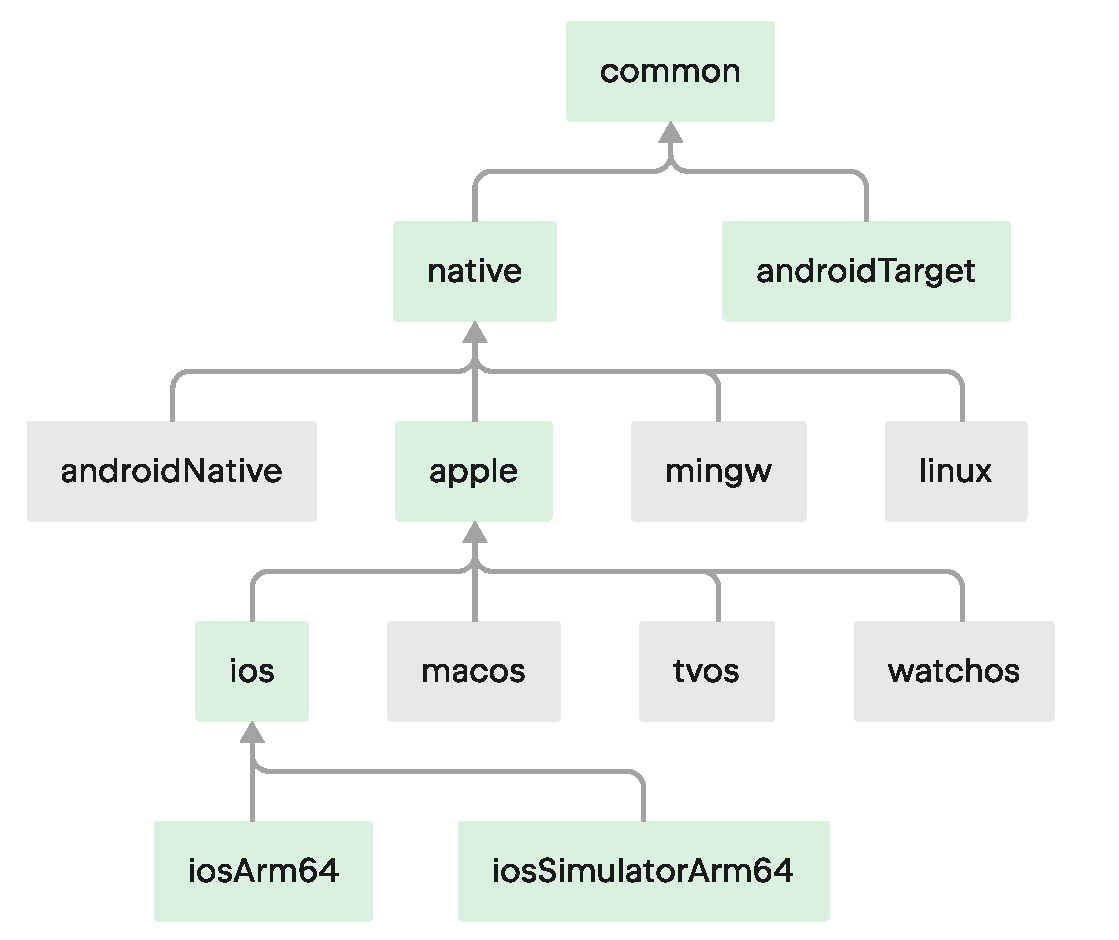
\includegraphics[width=1\linewidth]{figures/mptargets.pdf}
     \caption{Esempio di una possibile gerarchia di \textit{target}. Fonte: \url{https://archive.is/eH6ha}}
    \label{fig:targets}
 \end{figure}
Inoltre, questo meccanismo permette di applicare un \textit{template method} architetturale, grazie al quale è possibile dichiarare nel \textit{source set} \texttt{commonMain}
funzioni agnostiche tramite la direttiva \texttt{expected}, senza definirne il contenuto, che sarà valorizzato in un successivo momento.
In fase di compilazione, nelle versioni platform-specific, saranno valorizzate tramite funzioni che adottano la direttiva \texttt{actual},
che posso richiamare funzionalità altrimenti non disponibili in \texttt{commonMain}.
Una logica analoga è applicabile anche alla sezione dei test: sono disponibili un \textit{source set} di base, detto \texttt{commonTest}, e altri
eventuali che contengono codice compatibile solo nella relativa piattaforma.
In figura \ref{fig:sourcesetscompilation} viene mostrato il flusso e gli output ottenuti utilizzando i \textit{target} \texttt{JVM} e \texttt{JS}.

\begin{figure}[H]
    \centering
     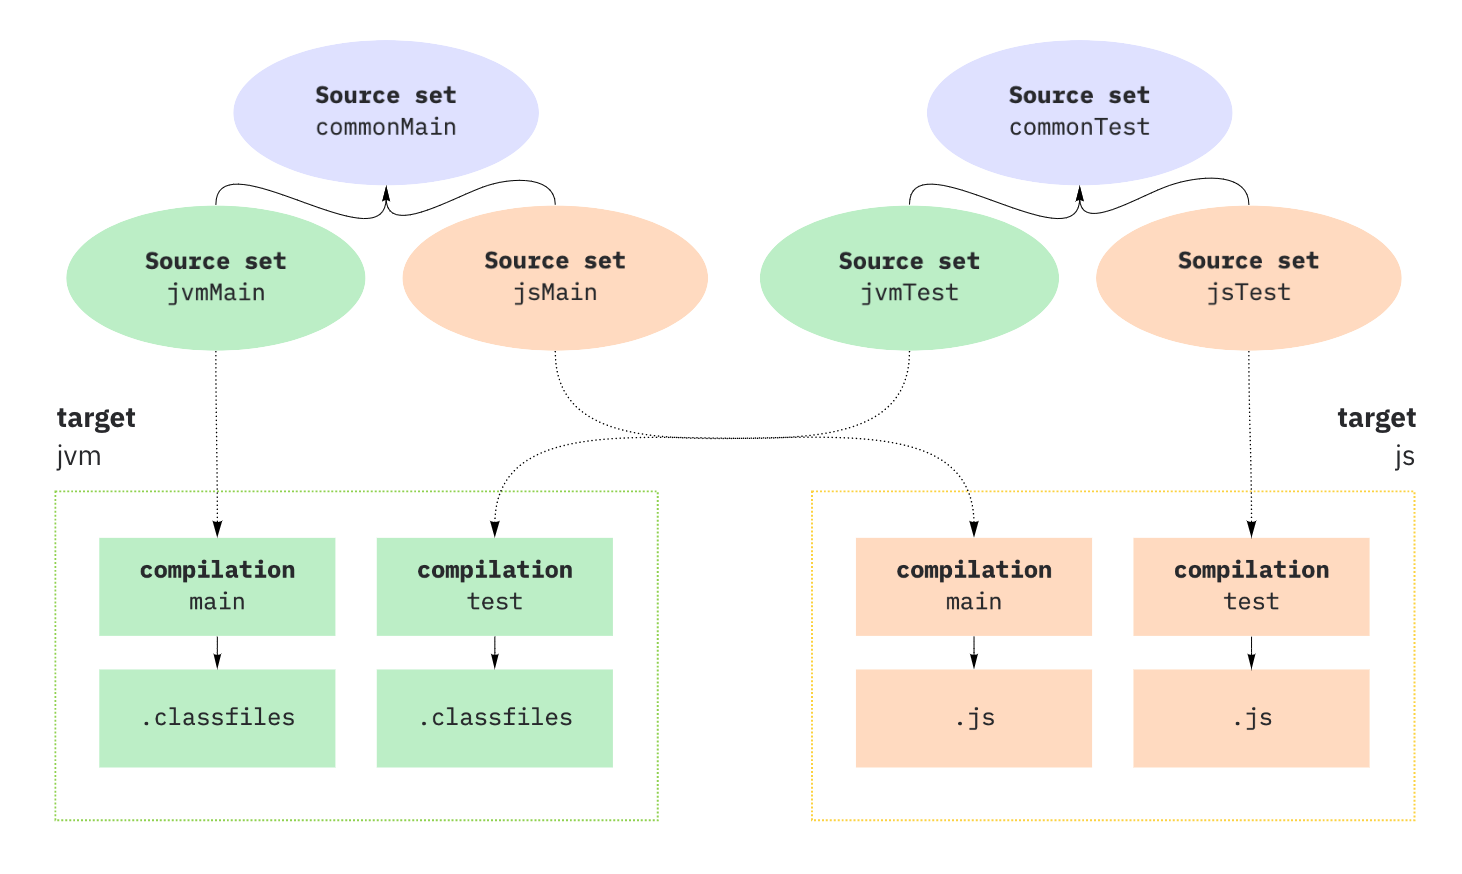
\includegraphics[width=1\linewidth]{figures/sourcesetscompilation.png}
     \caption{Esempio di output ottenibili in un progetto multipiattaforma. Fonte: \url{https://archive.is/wSykW}}
    \label{fig:sourcesetscompilation}
 \end{figure}

\subsection{GitHub Actions}
\ac{gha} è una piattaforma di \ac{ci}/\ac{cd} basata su repository \ac{gh},
ai quali possono essere agganciati degli elementi detti \textit{workflow}.
Un \textit{workflow}, definibile attraverso la sintassi \texttt{YAML}, rappresenta una sequenza di azioni che possono essere eseguite
all'occorrenza di un evento, ad esempio la creazione di un \textit{tag} nel repository,
una \textit{richiesta pull}, un'esecuzione manuale richiesta dal proprietario del repository, ecc\dots
In ogni \textit{workflow} va specificato il nome dello stesso e l'insieme di eventi che ne scatena 
l'esecuzione. 
Di seguito a ciò, è possibile definire un insieme di \textit{job}.
Ciascun \textit{job} è legato ad uno specifico ambiente di esecuzione: va definito che tipo di
sistema operativo deve essere adottato (\texttt{Linux}, \texttt{Windows}, \texttt{macOS})
e se al termine dello stesso debba essere restituito un output, che sarà accessibile da altri \textit{job}.
È possibile specificare delle variabili in una \textit{matrice}, in modo eseguire parallelamente molteplici istanze di uno stesso \textit{job} 
in base alle combinazioni delle variabili; a titolo esemplificativo, eseguire la compilazione di codice utilizzando
la stessa versione del compilatore ma su tre sistemi operativi differenti.  
Ciascun \textit{job} è caratterizzato da un proprio flusso indipendente, di conseguenza
per orchestare i processi è opportuno specificare condizioni basate sulle variabili di output 
oppure sull'indicazione del completamento di uno o più i \textit{jobs} desiderati.
All'interno del \textit{job} sono definibili uno o più \textit{step}: questi vengono eseguiti in maniera sequenziale
e sono impostabili per eseguire una sequenza arbitraria di comandi \texttt{bash} oppure
per eseguire una \textit{action} pubblica.
Quest'ultima rappresenta un ottimo modo di favorire il riuso
e la condivisione di codice nella community \ac{gh}, in quanto è possibile, ad esempio, utilizzare un \textit{workflow} complesso
come se fosse un singolo step (\textit{composite action}) oppure lanciare l'esecuzione di un container senza
imporre \textit{effort} riguardo alla gestione delle dipendenze e delle configurazioni (\textit{docker container action}).
\subsection{GitHub Pages}
\ac{ghpages} è un servizio di hosting disponibile per ogni account ed organizzazione in \ac{gh},
attraverso il quale è possibile pubblicare un sito web statico e renderlo accessibile tramite un webserver.
La pubblicazione avviene attraverso un apposito \textit{workflow} predefinito.
Nel caso di un iniziativa progettuale come una libreria, può essere utilizzato per dare informazioni 
su come scaricare ed installare il software oppure per pubblicare la documentazione.
\subsection{Maven Central, GitHub Packages e NPM}
Maven Central è tra i repository centralizzati più popolari per distribuire e riutilizzare artefatti basati su \texttt{\ac{jvm}}.
Un repository è definibile come "la directory che memorizza tutti i progetti e le librerie JAR, i plugin
o qualsiasi altro artefatto specifico del progetto che può essere facilmente utilizzato da Maven"~\cite{kozak2022three}.
Il sistema di gestione delle dipendenze di Maven è in grado di risolvere automaticamente le dipendenze transitive,
semplificando la gestione manuale delle dipendenze per gli sviluppatori. 
Gli artefatti caricati su Maven Central, tra cui librerie di codice compilato, documentazione ed elenco di dipendenze,
sono immutabili e non possono essere modificati né eliminati.
Gli artefatti vengono identificati univocamente con una tripletta \textit{groupId:artifactId:version},
dove \textit{groupId} identifica un gruppo di artefatti, \textit{artifactId} si riferisce al nome della libreria
e \textit{version} identifica univocamente ogni rilascio della libreria.
Ad esempio, la tripletta 'org.jetbrains.kotlinx:kotlinx-serialization-json:1.6.0' 
identifica la versione 1.6.0 di un serializzatore json per \texttt{Kotlin}, gestito da \texttt{JetBrains}.
Tutte le versioni di una libreria rilasciate su Maven Central sono sempre disponibili nel repository. 
Gli utenti della libreria sono liberi di decidere quale versione utilizzare e per quanto tempo e a questi ultimi è delegata la responsabilità di aggiornare le proprie dipendenze per 
adeguarsi a problemi di sicurezza o evoluzioni dell'API.
Nel lungo termine, queste decisioni determinano le librerie e le versioni più popolari nell'intero ecosistema software.
Si osserva che per la maggior parte delle librerie, più di una versione è attivamente utilizzata in un dato momento~\cite{soto2019emergence}. 
Dallo studio empirico condotto in~\cite{soto2019emergence}, è emerso che "circa il 40\% delle librerie ha due o più versioni attivamente utilizzate, 
mentre quasi il 4\% non ha mai avuto alcun utente su Maven Central. 
Inoltre, si è scoperto che più del 90\% delle versioni più popolari non sono le ultime versioni rilasciate, 
e sia le versioni attive che quelle significativamente popolari sono distribuite lungo la storia delle versioni della libreria".

Un'alternativa all'uso di Maven Central consiste in \ac{ghpackages}. Quest'ultimo pone una gestione 
semplificata per la pubblicazione degli artefatti, in quanto strettamente connesso all'uso di repository \ac{gh},
il che permette di avere un controllo degli accessi efficace come quello disponibile per i repo.
Al pari di Maven Central viene mantenuto il concetto di artefatti immutabili, e in più viene dato il supporto
per l'archiviazione di pacchetti in numerosi linguaggi, tra cui \texttt{C\#}.

Un altro famoso gestore di pacchetti è \ac{npm}, focalizzato sulle diffusione di librerie \texttt{\ac{js}} e \texttt{Node.js},
si differenzia dai precedenti in quanto non adotta il principio di immutabilità.
In questo caso, la modifica o eliminazione di una versione di un pacchetto può avere impatti\footnote{\url{https://archive.is/qMtZE}} notevoli sugli utilizzatori,
portando a potenziali disastri mondiali.


\section{Generazione multipiattaforma degli artefatti e pubblicazione}
La libreria EleKtion è stata realizzata partendo da un template\footnote{\url{https://archive.is/rLXB0}} disponibile su \ac{gh}, che fornisce 
la struttura di avvio per un progetto multipiattaforma in \texttt{Kotlin}, volto alla generazione e pubblicazione di artefatti.
I \textit{target} sono tutti compilati per \texttt{\ac{jvm} versione 1.8}, successivamente vengono anche convertiti in \texttt{\ac{js}} per la generazione della
libreria in ambito Web, e viene generata la versione \texttt{native}, compatibile in linguaggio nativo con i seguenti sistemi:
\begin{itemize}
    \label{list:elencotargetgenerati}
    \item{Linux x64;}
    \item{linux arm64;}
    \item{mingw x64;}
    \item{macos x64;}
    \item{macos arm64;}
    \item{ios arm64;}
    \item{ios x64;}
    \item{ios simulator arm64;}
    \item{watchos arm32;}
    \item{watchos x64;}
    \item{watchos simulator arm64;}
    \item{tvos arm64;}
    \item{tvos x64;}
    \item{tvos simulator arm64.}
\end{itemize}
Il processo di compilazione viene eseguito grazie ai \textit{workflow} presenti nel repository \ac{gh}:
il primo \textit{workflow}, definito \texttt{dispatcher}, viene avviato al momento della ricezione di un comando \textit{push} o della creazione di
una \textit{richiesta pull}, e richiama i seguenti \textit{workflow}:
\begin{enumerate}
\item{\texttt{build-and-deploy}: compila i sorgenti ed esegue i test nelle piattaforme dichiarate, effettua controlli di correttezza del codice
ed infine pubblica gli artefatti generati;}
\item{\texttt{publish-docs}: genera la documentazione degli artefatti e la mette a disposizione per la pubblicazione.}
\end{enumerate}
I \textit{workflow} \texttt{dispatcher} e \texttt{build-and-deploy} sono forniti dal template ma sono stati opportunamente configurati per lo scopo del progetto,
mentre il \textit{workflow} \texttt{publish-docs} è stato creato ex-novo.
\subsection{Generazione e pubblicazione della libreria}
Il \textit{workflow} \texttt{build-and-deploy} si occupa inizialmente di
calcolare la nuova versione da associare
alla libreria per poi inizializzare un repository di stage su Maven Central.
Successivamente viene lanciato il \textit{task} \texttt{gradle build} utilizzando una matrice con i sistemi operativi
 \texttt{windows-2022}, \texttt{macos-12}, \texttt{ubuntu-22.04}. Ciò permette di compilare il codice sorgente, 
 eseguire i test, effettuare i controlli di \texttt{code linting} e \texttt{bug detection} e generare gli artefatti
 in ciascun ambiente. Questi sono generati sulla base dei \textit{target} definiti nella lista al paragrafo \ref{list:elencotargetgenerati};
ciascun ambiente di compilazione, a seconda del sistema operativo in esecuzione, genera un \textit{subset} di artefatti e li carica sul repository di stage.
Infine il repository di stage viene chiuso e finalizzato. 
La finalizzazione del repository porta all'effettiva pubblicazione su Maven Central e si prosegue a pubblicare gli artefatti
anche su \ac{npm} e \ac{gh} Packages.
Completato questo flusso si prosegue ad invocare il \textit{workflow} \texttt{publish-docs}.
\subsection{Generazione e pubblicazione della documentazione}
Il \textit{workflow} \texttt{publish-docs} provvede alla generazione della documentazione, sulla base del codice presente
nel branch \texttt{master}. 
Al termine del \textit{workflow} \texttt{build-and-deploy} viene generato un \textit{tag}
associato al \textit{merge commit} effettuato sul branch \texttt{master}. Questo \textit{tag}
rappresenta il nuovo valore della versione appena rilasciata, il quale viene riportato nelle pagine di documentazione
generate attraverso il \textit{task} \texttt{gradle dokkaHtml}.
Queste pagine compongono un sito web statico e vengono copiate nel branch \texttt{gh-pages} grazie ad un'
apposita \textit{action}\footnote{\url{https://archive.is/NKNH0}}. 
La presenza di una modifica in questo branch scatena l'esecuzione di un \textit{workflow} di default,
che mette a disposizione il contenuto tramite un webserver, accessibile all'indirizzo https://corinz97.github.io/EleKtion/ .
In figura \ref{fig:dokkaSchermata} viene mostrato come appare il sito web statico al termine delle operazioni.
\begin{figure}
    \centering
   
     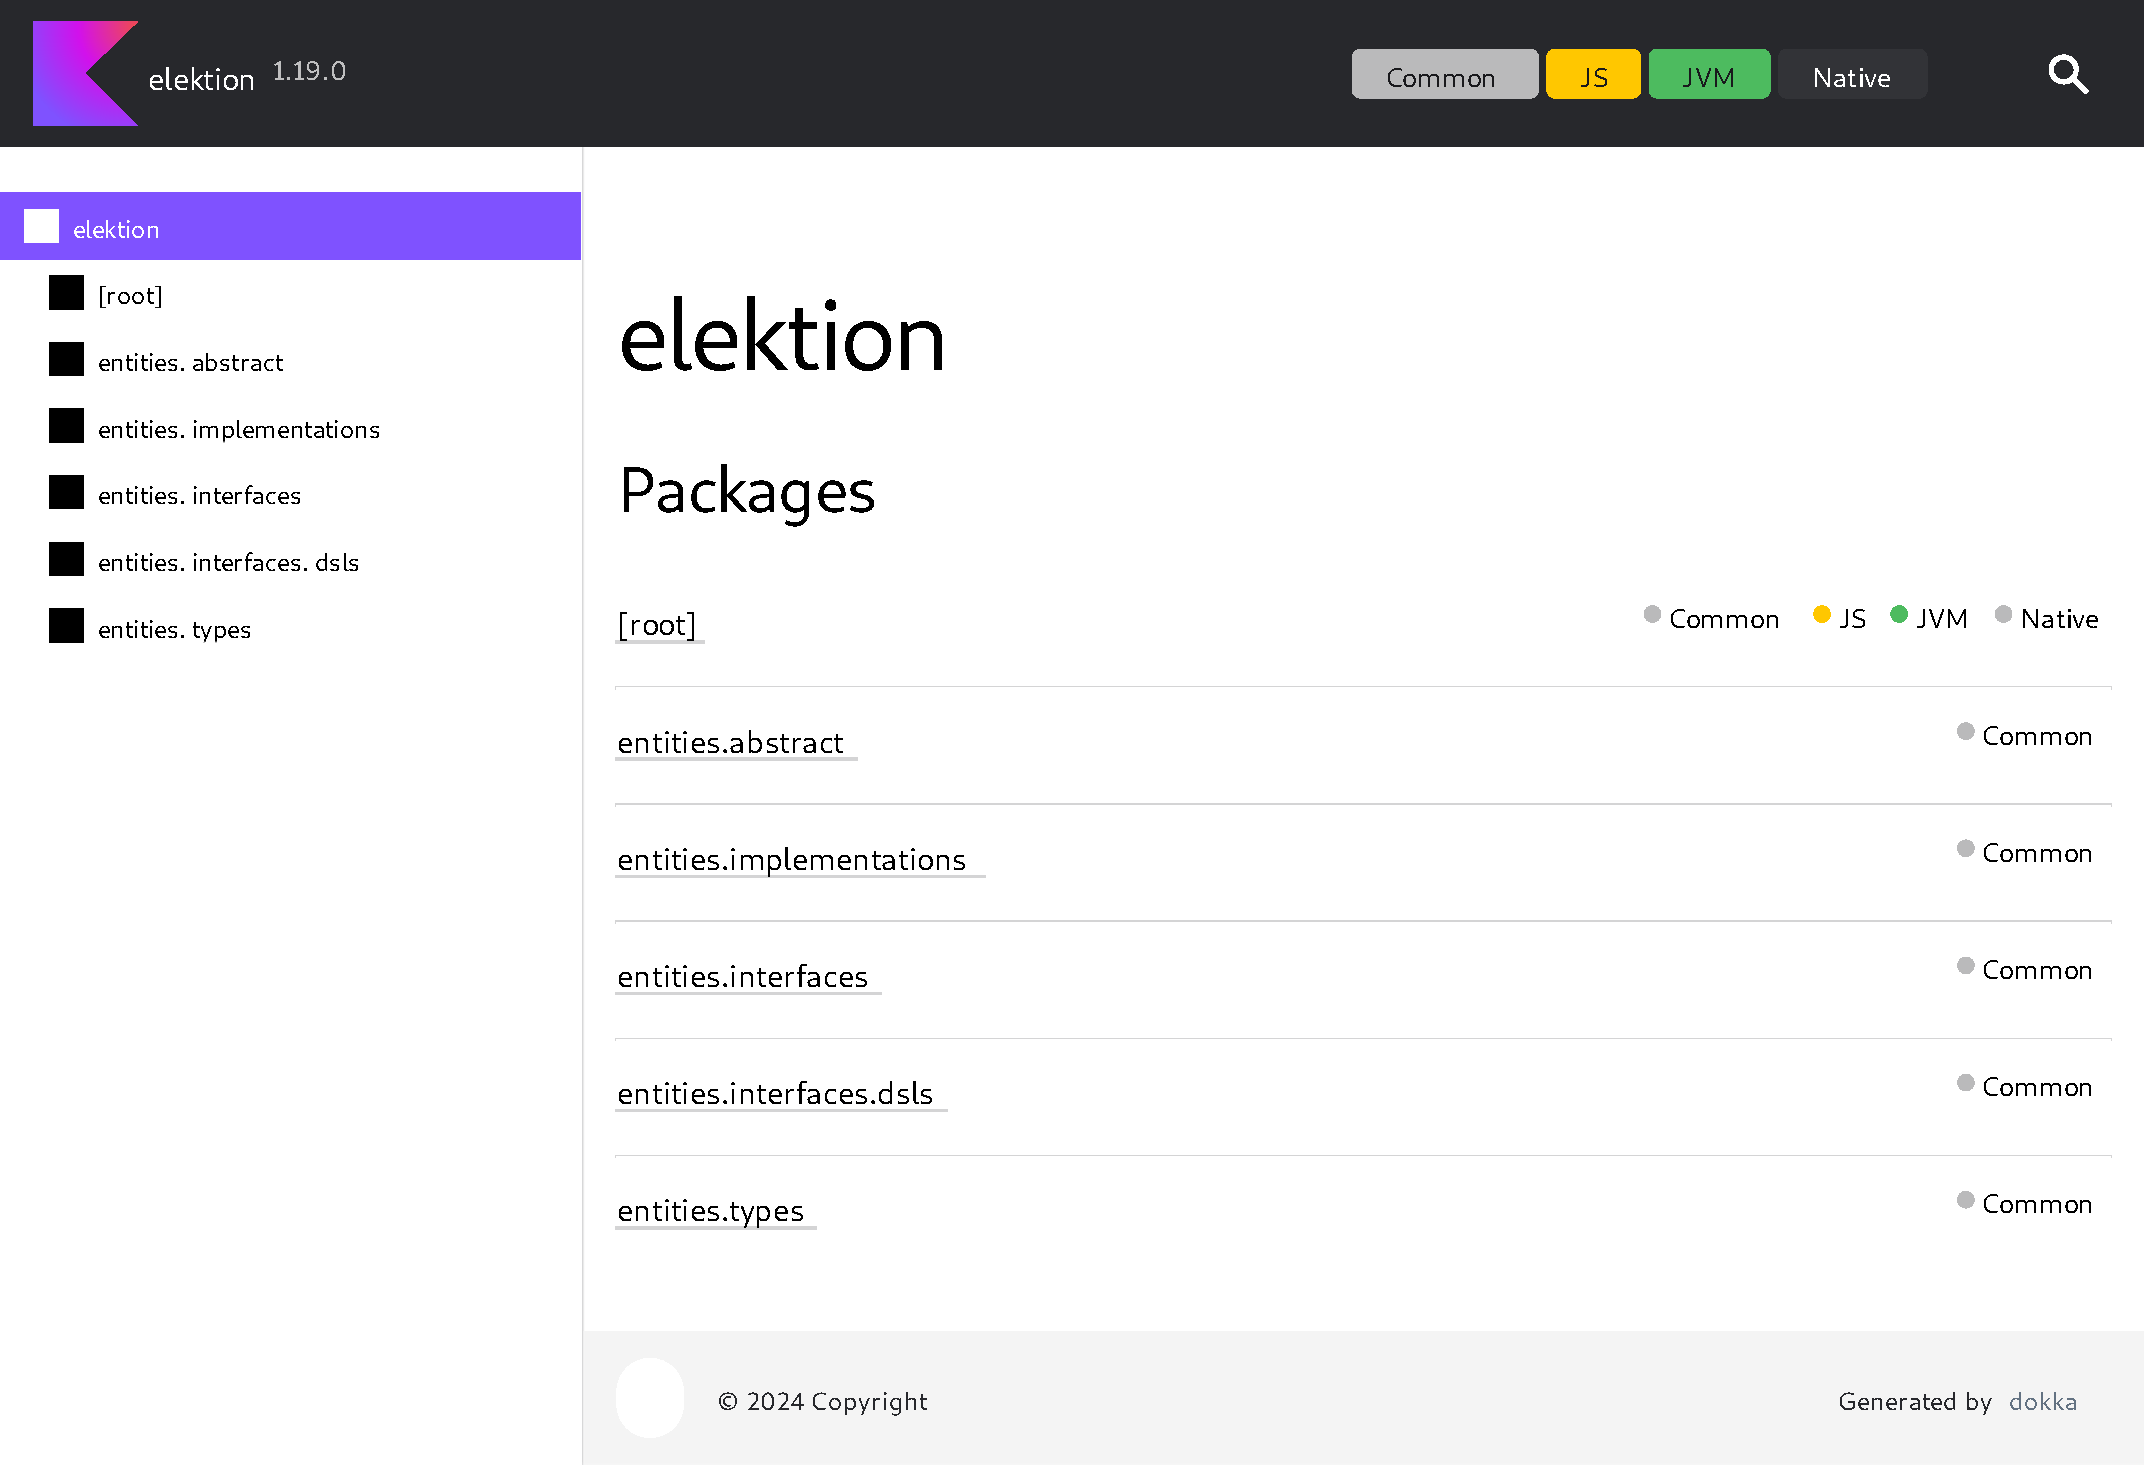
\includegraphics[width=1.05\linewidth]{figures/schermatadocumentazione.pdf}
     \caption{Sito web della documentazione, reso disponibile tramite \ac{ghpages} }
     \label{fig:dokkaSchermata}
 \end{figure}
%----------------------------------------------------------------------------------------


\chapter{Sperimentazione con i dati della Formula 1}
La sperimentazione della libreria EleKtion è stata estesa ad un
caso di studio reale, applicando gli algoritmi di votazione ai risultati 
delle gare di \ac{f1}.
I dati sono accessibili attraverso un API REST pubblica chiamata Ergast API\footnote{\url{https://archive.is/Iujgc}},
creata per scopi non-commerciali,
che mette a disposizione dati inerenti ai mondiali di \ac{f1} a partire dall'anno 1950.
Per ognuno di questi sono a disposizione numerose informazioni come l'elenco delle gare ufficiali (Gran Premi),
le gare di qualifica, le classifiche dei piloti, lo storico
dei piloti, le classifiche dei costruttori e molto altro.
Allo scopo di questa tesi, sono utili le informazioni riguardo ai risultati delle gare ufficiali
e le classifiche provvisorie dei piloti al termine di ogni gara, entrambe legate ad uno specifico anno.
Attaverso appositi endpoint, è possibile ottenere i dati necessari per predisporre le informazioni necessarie
ad EleKtion, utilizzando gli esiti delle varie gare come voti e applicando di conseguenza gli algoritmi a lista di preferenze.
L'elemento più favorito nel voto è rappresentato dal pilota che si è classificato primo in gara, mentre l'elemento più sfavorito
è il pilota classificatosi ultimo in gara.
Nei seguenti paragrafi vengono mostrati i passaggi effettuati per elaborare i dati di un mondiale,
in particolare vengono generate, come output delle votazioni, le classifiche provvisorie al termine di ogni gara in modo da avere uno storico,
che verrà confrontato con lo storico delle classifiche reali.
Verrà infine svolto un calcolo utile ad indicare
la differenza, in termini qualitativi, confrontando i risultati ottenuti.
\section{Elaborazione dati di un mondiale F1}
\label{paragrafoelaborazionemondiale}
Si è provveduto ad ottenere l'elenco delle gare svoltesi nel corso del mondiale AAAA (anno del mondiale), disponibili
all'endpoint di Ergast API \newline https://ergast.com/api/f1/AAAA.json.
In questo mondiale sono state effettuate in totale \textit{k} gare, per ognuna di esse sono stati scaricati i relativi
dati, filtrandoli, tenendo in considerazione solamente il nominativo del pilota e la posizione di arrivo.
Eventuali ritiri a causa di guasti o altri motivi non sono gestiti, ciascun pilota in ogni caso ha attribuita una posizione di arrivo.
I dati sono associati ad una mappa \texttt{Map<String, List<Pair<String, Int>>>}, nella quale le chiavi rappresentano
il nome della gara (es. Australian-Grand-Prix-1-AAAA, Malaysian-Grand-Prix-2-AAAA, ecc...) mentre i valori rappresentano liste
di tuple contenenti il nominativo del pilota e la posizione di arrivo.
Come mostrato nell'estratto di codice \ref{lst:election-GPs}, si organizzano tante votazioni indipendenti quante sono le
gare presenti nel mondiale:
viene definito l'insieme dei nominativi presenti nel mondiale, in modo da
avere il censimento di tutti coloro che hanno partecipato almeno in una gara.
 Si definisce l'algoritmo da utilizzare, e in questo caso di studio sono
ammissibili l'algoritmo di Condorcet o l'algoritmo di Schultze. 
Successivamente si determina l'elenco dei voti, in cui i votati
sono costituiti dall'elenco dei nominativi dei piloti secondo l'ordine di arrivo reale (dal primo all'ultimo), e come votante viene utilizzato il nome del circuito
della gara. Se uno o più piloti sono assenti in quella gara ma presenti in altre, tramite un confronto con l'insieme dei candidati
vengono identificati e posti "virtualmente" ad ultimi in modo da avere la lunghezza della lista 
di preferenze uniforme al numero dei candidati.
Infine, questa votazione viene inserita nell'elenco delle votazioni da elaborare.
Per la seconda votazione viene considerata anche la seconda gara, e mantenendo stabile l'insieme dei candidati e l'algoritmo selezionato,
vengono considerati come voti l'elenco dei nominativi (secondo l'ordine di arrivo reale) della prima gara
e l'elenco dei nominativi (secondo l'ordine di arrivo reale) della seconda gara.
Proseguendo nelle iterazioni, si arriva ad avere \textit{k} votazioni indipendenti, in cui l'ultima conterrà
come voti gli esiti dalla prima alla \textit{k}-esima gara.
La generazione delle classifiche provvisorie fornisce una serie di risultati in
cui il primo consiste nella classifica provvisoria al termine della prima gara, il secondo nella classifica provvisoria al termine 
della seconda gara, fino ad arrivare alla classifica finale.
I dati delle classifiche provvisorie reali sono ottenuti contattando l'endpoint \newline https://ergast.com/api/f1/AAAA/GP/driverStandings.json,
dove AAAA è l'anno del mondiale e GP è il numero della gara
\lstinputlisting[language=Kotlin,label={lst:election-GPs}, caption={Generazione delle classifiche provvisorie utilizzando EleKtion}]{listings/election-GPs.kt}
Per confrontare gli esiti ottenuti impiegando i differenti algoritmi e quelli reali estratti dall'API,
è necessario organizzarli secondo matrici \textit{r x k}, dove ogni riga \textit{r} identifica un pilota,
e ogni colonna \textit{k} identifica una gara. Nell'intersezione è presente la
posizione nella classifica provvisoria (reale o generata) ottenuta dal \textit{r}-esimo pilota al termine della
\textit{k}-esima gara.
Per effettuare un confronto qualitativo tra matrici è fondamentale organizzarle in modo tale che le righe e le colonne
siano ordinate allo stesso modo. Nel caso delle righe è possibile adottare un ordinamento lessicografico o 
l'ordinamento presente in una delle matrici, che viene preso come riferimento per le altre.
Nella sperimentazione effettuata, sono state calcolate per prime le classifiche che impiegano l'algoritmo di Condorcet,
poi la sequenza dei piloti nella classifica finale è stato preso come riferimento di ordinamento.
Le classifiche ottenute con l'algoritmo di Schultze sono state organizzate secondo lo stesso riferimento e così anche
le classifiche reali. Si rimanda agli estratti di codice \ref{lst:ordering-rankings-condorcet}, \ref{lst:ordering-rankings-schultze},
\ref{lst:ordering-rankings-real} per approfondire l'implementazione di questo ordinamento.
Esistono numerose metriche di confronto tra matrici~\cite{golub2013matrix}, in questo caso si è optato per la \textit{norma di Frobenius},
rappresentata dalla formula $\sqrt{\sum_{i,j}^{} abs(a_{i,j})^2}$, dove $a_{i,j}$ è l'elemento di una matrice $A$ ricavata dalla
differenza tra le matrici trattate.
\lstinputlisting[language=Kotlin,label={lst:ordering-rankings-condorcet}, caption={Ordinamento propedeutico al confronto (Condorcet)}]{listings/ordering-rankings-Condorcet.kt}
\lstinputlisting[language=Kotlin,label={lst:ordering-rankings-schultze}, caption={Ordinamento propedeutico al confronto (Schultze)}]{listings/ordering-rankings-Schultze.kt}
\lstinputlisting[language=Kotlin,label={lst:ordering-rankings-real},caption={Ordinamento propedeutico al confronto (Dati reali)}]{listings/ordering-rankings-real.kt}
\section{Elaborazione del mondiale F1 2023}
Si è provveduto alla generazione delle classifiche provvisorie utilizzando i dati del mondiale F1 2023.
Si riporta in tabella \ref{table:classifichefinali2023} la classifica finale reale e quelle 
finali basate sull'algoritmo di Condorcet e l'algoritmo di Schultze.
%%2023
\begin{table}[H]
    \centering
    \begingroup
    \resizebox{\linewidth}{!}{%
    \begin{tabular}{|p{0.1\linewidth}|p{0.33\linewidth}|p{0.33\linewidth}|p{0.33\linewidth}|}

    \hline
    \multicolumn{1}{|l|}{Posizione} & \multicolumn{1}{l|}{Reali} & \multicolumn{1}{l|}{Condorcet} & \multicolumn{1}{l|}{Schultze} \\ \hline
    1.	 & 	Max-Verstappen  & 	 Max-Verstappen (C1.)& 	 Max-Verstappen 	 \\ \hline
    2.	 & 	Sergio-Pérez & 	 Sergio-Pérez (C2.) & 	 Sergio-Pérez 	 \\ \hline
    3.	 & 	Lewis-Hamilton & 	 Lewis-Hamilton (C3.)& 	 Lewis-Hamilton 	 \\ \hline
    4.	 & 	Fernando-Alonso & 	 Fernando-Alonso (C4.)\newline Carlos-Sainz (C5.) \newline Charles-Leclerc (C6.) & 	 Fernando-Alonso 	 \\ \hline
    5.	 & 	Charles-Leclerc & 	 Lando-Norris (C7.) & 	 Carlos-Sainz 	 \\ \hline
    6.	 & 	Lando-Norris & 	 George-Russell (C8.)& 	 Lando-Norris 	 \\ \hline
    7.	 & 	Carlos-Sainz & 	 Lance-Stroll (C9.)\newline Oscar-Piastri (C10.) & 	 George-Russell 	 \\ \hline
    8.	 & 	George-Russell & 	 Pierre-Gasly (C11.) & 	 Charles-Leclerc 	 \\ \hline
    9.	 & 	Oscar-Piastri & 	 Alexander-Albon (C12.) \newline Esteban-Ocon (C13.) & 	 Pierre-Gasly 	 \\ \hline
    10.	 & 	Lance-Stroll & 	 Yuki-Tsunoda (C14.) & 	 Oscar-Piastri 	 \\ \hline
    11.	 & 	Pierre-Gasly & 	 Valtteri-Bottas (C15.)\newline Nico-Hülkenberg (C16.) & 	 Lance-Stroll 	 \\ \hline
    12.	 & 	Esteban-Ocon & 	 Guanyu-Zhou (C17.) & 	 Esteban-Ocon 	 \\ \hline
    13.	 & 	Alexander-Albon & 	 Kevin-Magnussen (C18.) & 	 Alexander-Albon 	 \\ \hline
    14.	 & 	Yuki-Tsunoda & 	 Logan-Sargeant (C19.) & 	 Yuki-Tsunoda 	 \\ \hline
    15.	 & 	Valtteri-Bottas & 	 Nyck-de Vries (C20.)& 	 Valtteri-Bottas 	 \\ \hline
    16.	 & 	Nico-Hülkenberg & 	 Daniel-Ricciardo (C21.)& 	 Guanyu-Zhou 	 \\ \hline
    17.	 & 	Daniel-Ricciardo & 	 Liam-Lawson (C22.) &	 Nico-Hülkenberg 	 \\ \hline
    18.	 & 	Guanyu-Zhou & 	 Assente &	 Kevin-Magnussen 	 \\ \hline
    19.	 & 	Kevin-Magnussen & 	 Assente &	 Logan-Sargeant 	 \\ \hline
    20.	 & 	Liam-Lawson & 	 Assente &	 Daniel-Ricciardo 	 \\ \hline
    21.	 & 	Logan-Sargeant & 	 Assente &	 Nyck-de Vries 	 \\ \hline
    22.	 & 	Nyck-de Vries & 	 Assente &	 Liam-Lawson 	 \\ \hline
    
    

    \end{tabular}}
    \endgroup

    \caption{Classifica finale reale e classifiche finali ottenute con 
    l'algoritmo di Condorcet e l'algoritmo di Schultze, relativamente al mondiale F1 2023.
    Nella colonna relativa all'algoritmo di Condorcet viene fornito un acronimo ad ogni concorrente. }
    \label{table:classifichefinali2023}
\end{table}
Nelle tabelle \ref{table:classifichegeneralireali2023tabella}, \ref{table:classifichegeneralicondorcet2023tabella} e \ref{table:classifichegeneralischultze2023tabella}
vengono mostrate le matrici complete con il posizionamento dei piloti in ogni classifica provvisoria.
Per motivi prettamente grafici, a ciascun concorrente è stato assegnato un acronimo, consultabile nella terza colonna della tabella \ref{table:classifichefinali2023} .
Infine, per ciascuna tabella è stato generato il relativo grafico, nel quale le linee rappresentano i concorrenti,
l'asse delle ascisse rappresenta il numero sequenziale della gara e l'asse delle ordinate è associato al posizionamento in classifica
al termine della relativa gara.
Per la tabella \ref{table:classifichegeneralireali2023tabella} il grafico di riferimento è in figura \ref{fig:classifichegeneralireali2023figura},
mentre per le tabelle \ref{table:classifichegeneralicondorcet2023tabella} e \ref{table:classifichegeneralischultze2023tabella} i grafici sono rispettivamente
in figura \ref{fig:classifichegeneralicondorcet2023figura} ed in figura \ref{fig:classifichegeneralischultze2023figura}.
\begin{table}[H]
    \centering
    \begingroup
    \resizebox{\linewidth}{!}{%
    \begin{tabular}{|c|c|c|c|c|c|c|c|c|c|c|c|c|c|c|c|c|c|c|c|c|c|c|}

    \hline
    \multicolumn{1}{|l|}{} & \multicolumn{1}{l|}{G1} & \multicolumn{1}{l|}{G2} & \multicolumn{1}{l|}{G3} & \multicolumn{1}{l|}{G4} & \multicolumn{1}{l|}{G5} & \multicolumn{1}{l|}{G6} & \multicolumn{1}{l|}{G7} & \multicolumn{1}{l|}{G8} & \multicolumn{1}{l|}{G9} & \multicolumn{1}{l|}{G10} & \multicolumn{1}{l|}{G11} & \multicolumn{1}{l|}{G12} & \multicolumn{1}{l|}{G13} & \multicolumn{1}{l|}{G14} & \multicolumn{1}{l|}{G15} & \multicolumn{1}{l|}{G16} & \multicolumn{1}{l|}{G17} & \multicolumn{1}{l|}{G18} & \multicolumn{1}{l|}{G19} & \multicolumn{1}{l|}{G20} & \multicolumn{1}{l|}{G21} & \multicolumn{1}{l|}{G22} \\ \hline
    C1. & 1 & 1 & 1 & 1 & 1 & 1 & 1 & 1 & 1 & 1 & 1 & 1 & 1 & 1 & 1 & 1 & 1 & 1 & 1 & 1 & 1 & 1 \\ \hline
    C2. & 2 & 2 & 2 & 2 & 2 & 2 & 2 & 2 & 2 & 2 & 2 & 2 & 2 & 2 & 2 & 2 & 2 & 2 & 2 & 2 & 2 & 2 \\ \hline
    C3. & 5 & 5 & 4 & 4 & 4 & 4 & 4 & 4 & 4 & 4 & 4 & 4 & 4 & 4 & 3 & 3 & 3 & 3 & 3 & 3 & 3 & 3 \\ \hline
    C4. & 3 & 3 & 3 & 3 & 3 & 3 & 3 & 3 & 3 & 3 & 3 & 3 & 3 & 3 & 4 & 4 & 4 & 4 & 5 & 4 & 5 & 4 \\ \hline
    C5. & 4 & 4 & 5 & 5 & 5 & 6 & 6 & 5 & 5 & 5 & 6 & 7 & 5 & 5 & 5 & 5 & 5 & 5 & 4 & 6 & 4 & 7 \\ \hline
    C6. & 19 & 8 & 10 & 6 & 7 & 7 & 7 & 7 & 6 & 7 & 7 & 5 & 6 & 6 & 6 & 6 & 6 & 7 & 7 & 7 & 7 & 5 \\ \hline
    C7. & 17 & 20 & 8 & 9 & 9 & 11 & 11 & 11 & 10 & 9 & 8 & 8 & 8 & 8 & 8 & 7 & 7 & 6 & 6 & 5 & 6 & 6 \\ \hline
    C8. & 7 & 6 & 7 & 7 & 6 & 5 & 5 & 6 & 7 & 6 & 5 & 6 & 7 & 7 & 7 & 8 & 8 & 8 & 8 & 8 & 8 & 8 \\ \hline
    C9. & 6 & 7 & 6 & 8 & 8 & 8 & 8 & 8 & 8 & 8 & 9 & 9 & 9 & 9 & 9 & 10 & 10 & 11 & 11 & 10 & 10 & 10 \\ \hline
    C10. & 20 & 19 & 13 & 11 & 14 & 13 & 13 & 14 & 14 & 11 & 11 & 11 & 12 & 12 & 11 & 9 & 9 & 9 & 9 & 9 & 9 & 9 \\ \hline
    C11. & 9 & 11 & 14 & 14 & 10 & 10 & 10 & 10 & 11 & 12 & 12 & 12 & 10 & 10 & 10 & 11 & 11 & 10 & 10 & 11 & 11 & 11 \\ \hline
    C12. & 10 & 13 & 18 & 17 & 18 & 18 & 18 & 12 & 13 & 13 & 13 & 13 & 13 & 13 & 13 & 13 & 13 & 13 & 13 & 13 & 13 & 13 \\ \hline
    C13. & 18 & 10 & 12 & 13 & 12 & 9 & 9 & 9 & 9 & 10 & 10 & 10 & 11 & 11 & 12 & 12 & 12 & 12 & 12 & 12 & 12 & 12 \\ \hline
    C14. & 11 & 14 & 16 & 16 & 16 & 16 & 16 & 17 & 17 & 17 & 17 & 17 & 17 & 17 & 17 & 17 & 17 & 16 & 16 & 14 & 14 & 14 \\ \hline
    C15. & 8 & 9 & 11 & 12 & 13 & 14 & 14 & 15 & 15 & 15 & 15 & 15 & 15 & 15 & 15 & 15 & 14 & 14 & 14 & 15 & 15 & 15 \\ \hline
    C16. & 15 & 15 & 9 & 10 & 11 & 12 & 12 & 13 & 12 & 14 & 14 & 14 & 14 & 14 & 14 & 14 & 15 & 15 & 15 & 16 & 16 & 16 \\ \hline
    C17. & 16 & 17 & 15 & 15 & 15 & 15 & 15 & 16 & 16 & 16 & 16 & 16 & 16 & 16 & 16 & 16 & 16 & 17 & 18 & 18 & 18 & 18 \\ \hline
    C18. & 13 & 12 & 17 & 18 & 17 & 17 & 17 & 18 & 18 & 18 & 18 & 18 & 18 & 18 & 18 & 18 & 18 & 18 & 19 & 19 & 19 & 19 \\ \hline
    C19. & 12 & 16 & 19 & 19 & 19 & 20 & 20 & 20 & 19 & 19 & 19 & 19 & 19 & 19 & 20 & 20 & 20 & 20 & 21 & 21 & 21 & 21 \\ \hline
    C20. & 14 & 18 & 20 & 20 & 20 & 19 & 19 & 19 & 20 & 20 & 20 & 20 & 20 & 21 & 21 & 21 & 21 & 21 & 22 & 22 & 22 & 22 \\ \hline
    C21. & 20 & 20 & 20 & 20 & 20 & 20 & 20 & 20 & 20 & 20 & 21 & 21 & 21 & 22 & 22 & 22 & 22 & 22 & 17 & 17 & 17 & 17 \\ \hline
    C22. & 20 & 20 & 20 & 20 & 20 & 20 & 20 & 20 & 20 & 20 & 21 & 21 & 22 & 20 & 19 & 19 & 19 & 19 & 20 & 20 & 20 & 20 \\ \hline
    \end{tabular}}
    \endgroup

    \caption{Tabella relativa ai valori reali del Mondiale F1 2023, in cui per ogni gara (G*)  è riportata la posizione del concorrente (C*) in classifica generale, al termine della gara stessa.
    I valori sono ricavati da Ergast API .}
    \label{table:classifichegeneralireali2023tabella}
\end{table}

\begin{figure}[H]
    \centering
     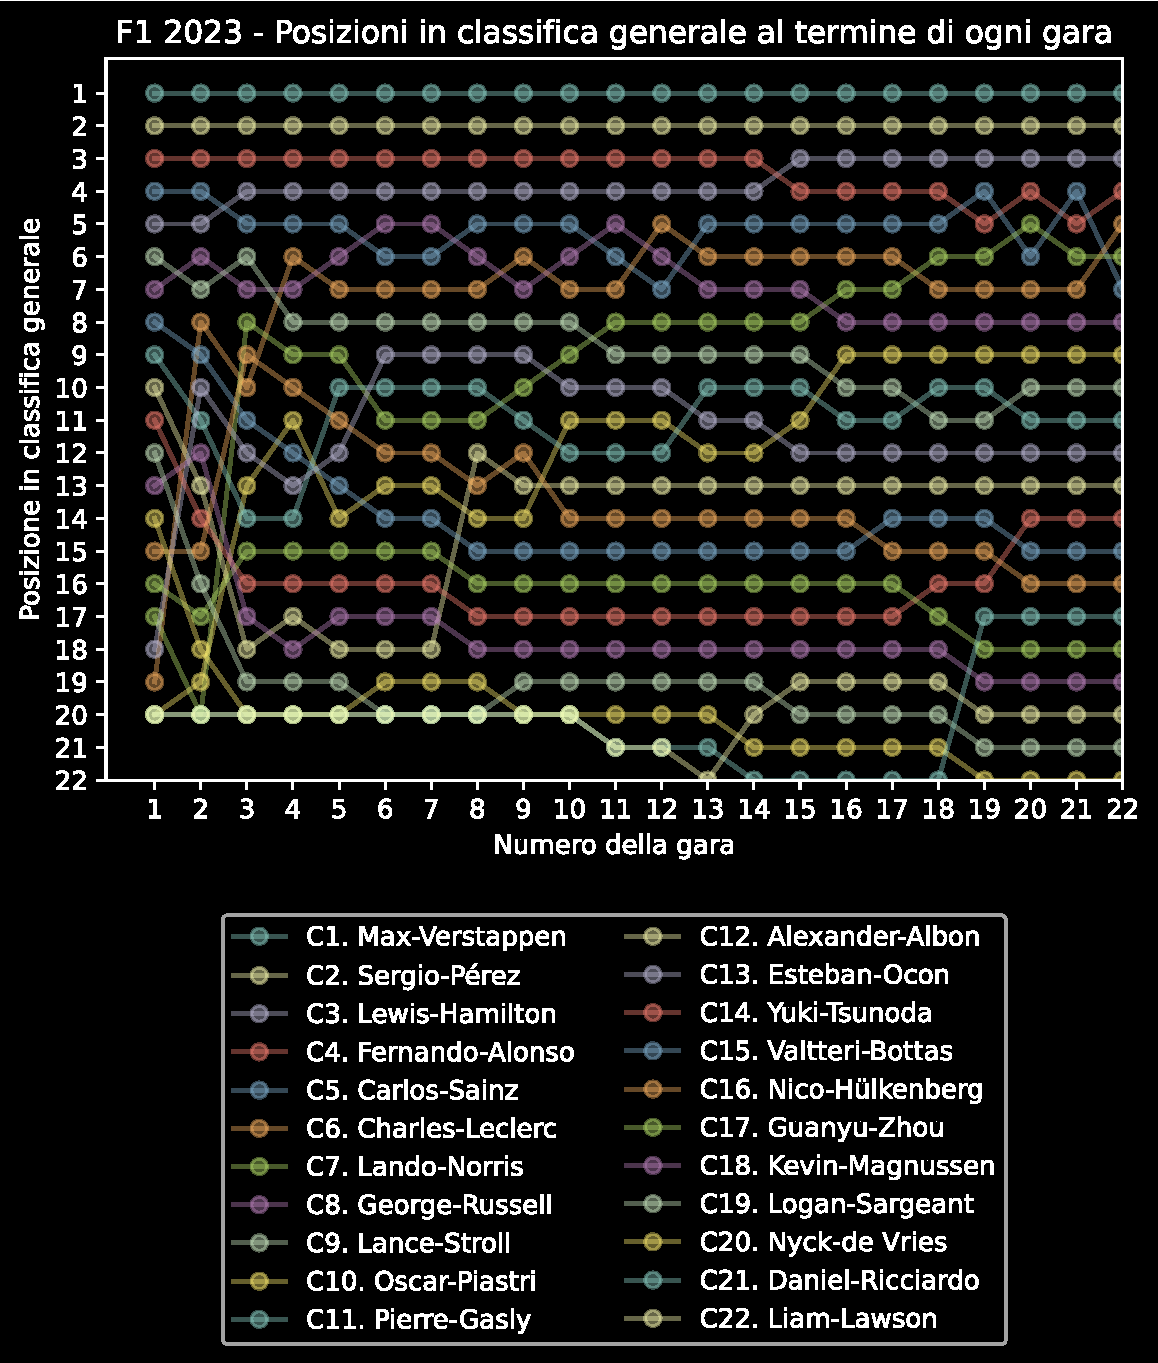
\includegraphics[width=\linewidth]{figures/realstandings2023.pdf}
     \caption{Rappresentazione grafica della tabella \ref{table:classifichegeneralireali2023tabella} }
     \label{fig:classifichegeneralireali2023figura}
 \end{figure}


 \begin{table}[H]
    \centering
    \begingroup
    \resizebox{\linewidth}{!}{%
    \begin{tabular}{|c|c|c|c|c|c|c|c|c|c|c|c|c|c|c|c|c|c|c|c|c|c|c|}

    \hline
    \multicolumn{1}{|l|}{} & \multicolumn{1}{l|}{G1} & \multicolumn{1}{l|}{G2} & \multicolumn{1}{l|}{G3} & \multicolumn{1}{l|}{G4} & \multicolumn{1}{l|}{G5} & \multicolumn{1}{l|}{G6} & \multicolumn{1}{l|}{G7} & \multicolumn{1}{l|}{G8} & \multicolumn{1}{l|}{G9} & \multicolumn{1}{l|}{G10} & \multicolumn{1}{l|}{G11} & \multicolumn{1}{l|}{G12} & \multicolumn{1}{l|}{G13} & \multicolumn{1}{l|}{G14} & \multicolumn{1}{l|}{G15} & \multicolumn{1}{l|}{G16} & \multicolumn{1}{l|}{G17} & \multicolumn{1}{l|}{G18} & \multicolumn{1}{l|}{G19} & \multicolumn{1}{l|}{G20} & \multicolumn{1}{l|}{G21} & \multicolumn{1}{l|}{G22} \\ \hline
    C1. & 1 & 1 & 1 & 1 & 1 & 1 & 1 & 1 & 1 & 1 & 1 & 1 & 1 & 1 & 1 & 1 & 1 & 1 & 1 & 1 & 1 & 1 \\ \hline
    C2. & 2 & 1 & 2 & 1 & 2 & 2 & 2 & 2 & 2 & 2 & 2 & 2 & 2 & 2 & 2 & 2 & 2 & 2 & 2 & 2 & 2 & 2 \\ \hline
    C3. & 5 & 3 & 4 & 3 & 5 & 4 & 4 & 3 & 4 & 3 & 4 & 4 & 4 & 4 & 4 & 3 & 4 & 4 & 4 & 3 & 4 & 3 \\ \hline
    C4. & 3 & 2 & 3 & 2 & 3 & 3 & 3 & 2 & 3 & 2 & 3 & 3 & 3 & 3 & 3 & 3 & 3 & 3 & 3 & 3 & 3 & 4 \\ \hline
    C5.  & 4 & 3 & 5 & 3 & 4 & 5 & 6 & 4 & 5 & 5 & 7 & 7 & 7 & 6 & 5 & 4 & 5 & 5 & 5 & 4 & 5 & 4 \\ \hline
    C6.  & 19 & 10 & 14 & 11 & 6 & 7 & 7 & 6 & 7 & 5 & 6 & 6 & 6 & 6 & 7 & 5 & 5 & 7 & 5 & 6 & 5 & 4 \\ \hline
    C7. & 17 & 11 & 13 & 7 & 11 & 10 & 11 & 10 & 11 & 8 & 10 & 9 & 8 & 7 & 8 & 6 & 6 & 6 & 6 & 5 & 6 & 5 \\ \hline
    C8. & 7 & 4 & 7 & 4 & 6 & 6 & 5 & 5 & 6 & 4 & 5 & 5 & 5 & 5 & 6 & 5 & 7 & 6 & 7 & 5 & 7 & 6 \\ \hline
    C9. & 6 & 11 & 6 & 4 & 6 & 9 & 7 & 7 & 8 & 6 & 8 & 8 & 8 & 7 & 9 & 9 & 9 & 10 & 9 & 9 & 8 & 7 \\ \hline
    C10.  & 20 & 11 & 14 & 8 & 15 & 12 & 12 & 10 & 13 & 10 & 11 & 12 & 9 & 10 & 11 & 8 & 8 & 9 & 8 & 8 & 9 & 7 \\ \hline
    C11. & 9 & 5 & 8 & 6 & 7 & 8 & 8 & 8 & 9 & 7 & 9 & 10 & 8 & 8 & 10 & 7 & 8 & 8 & 8 & 7 & 8 & 8 \\ \hline
    C12.  & 10 & 11 & 14 & 11 & 13 & 13 & 16 & 12 & 14 & 11 & 11 & 13 & 9 & 9 & 11 & 8 & 9 & 10 & 9 & 9 & 10 & 9 \\ \hline
    C13.  & 18 & 10 & 11 & 9 & 9 & 9 & 9 & 8 & 10 & 9 & 11 & 11 & 9 & 9 & 11 & 9 & 9 & 11 & 9 & 10 & 11 & 9 \\ \hline
    C14.  & 11 & 6 & 8 & 5 & 8 & 9 & 10 & 9 & 12 & 12 & 13 & 13 & 11 & 12 & 13 & 11 & 11 & 13 & 11 & 11 & 13 & 10 \\ \hline
    C15.  & 8 & 10 & 11 & 9 & 12 & 11 & 13 & 11 & 13 & 11 & 12 & 13 & 10 & 11 & 12 & 10 & 10 & 12 & 10 & 12 & 12 & 11 \\ \hline
    C16. & 15 & 8 & 9 & 7 & 10 & 11 & 11 & 12 & 15 & 13 & 14 & 14 & 12 & 13 & 14 & 12 & 12 & 14 & 12 & 12 & 14 & 11 \\ \hline
    C17.  & 16 & 9 & 10 & 10 & 13 & 12 & 14 & 13 & 15 & 13 & 15 & 14 & 13 & 14 & 15 & 13 & 13 & 15 & 13 & 13 & 15 & 12 \\ \hline
    C18. & 13 & 7 & 12 & 9 & 9 & 12 & 13 & 13 & 15 & 15 & 16 & 15 & 14 & 15 & 16 & 14 & 14 & 16 & 14 & 14 & 16 & 13 \\ \hline
    C19.  & 12 & 10 & 13 & 11 & 16 & 14 & 17 & 15 & 17 & 15 & 18 & 16 & 15 & 16 & 17 & 15 & 15 & 17 & 15 & 15 & 17 & 14 \\ \hline
    C20.  & 14 & 9 & 12 & 11 & 14 & 13 & 15 & 14 & 16 & 14 & 17 & 16 & 16 & 17 & 18 & 16 & 16 & 18 & 16 & 16 & 18 & 15 \\ \hline
    C21. & 21 & 12 & 15 & 12 & 17 & 15 & 18 & 16 & 18 & 16 & 19 & 17 & 17 & 18 & 19 & 17 & 17 & 19 & 17 & 17 & 19 & 16 \\ \hline
    C22.  & 22 & 13 & 16 & 13 & 18 & 16 & 19 & 17 & 19 & 17 & 20 & 18 & 18 & 19 & 20 & 18 & 18 & 20 & 18 & 18 & 20 & 17 \\ \hline
    \end{tabular}}
    \endgroup

    \caption{Tabella relativa al Mondiale F1 2023, in cui per ogni gara (G*)  è riportata la posizione del concorrente (C*) in classifica, al termine della gara stessa.
    I valori sono ricavati dall'applicazione dell'algoritmo di Condorcet al termine di ogni gara, considerando anche le precedenti.
    Ogni gara rappresenta un voto, composto dagli ordini di arrivo.
    }
    \label{table:classifichegeneralicondorcet2023tabella}
\end{table}

\begin{figure}[H]
    \centering
     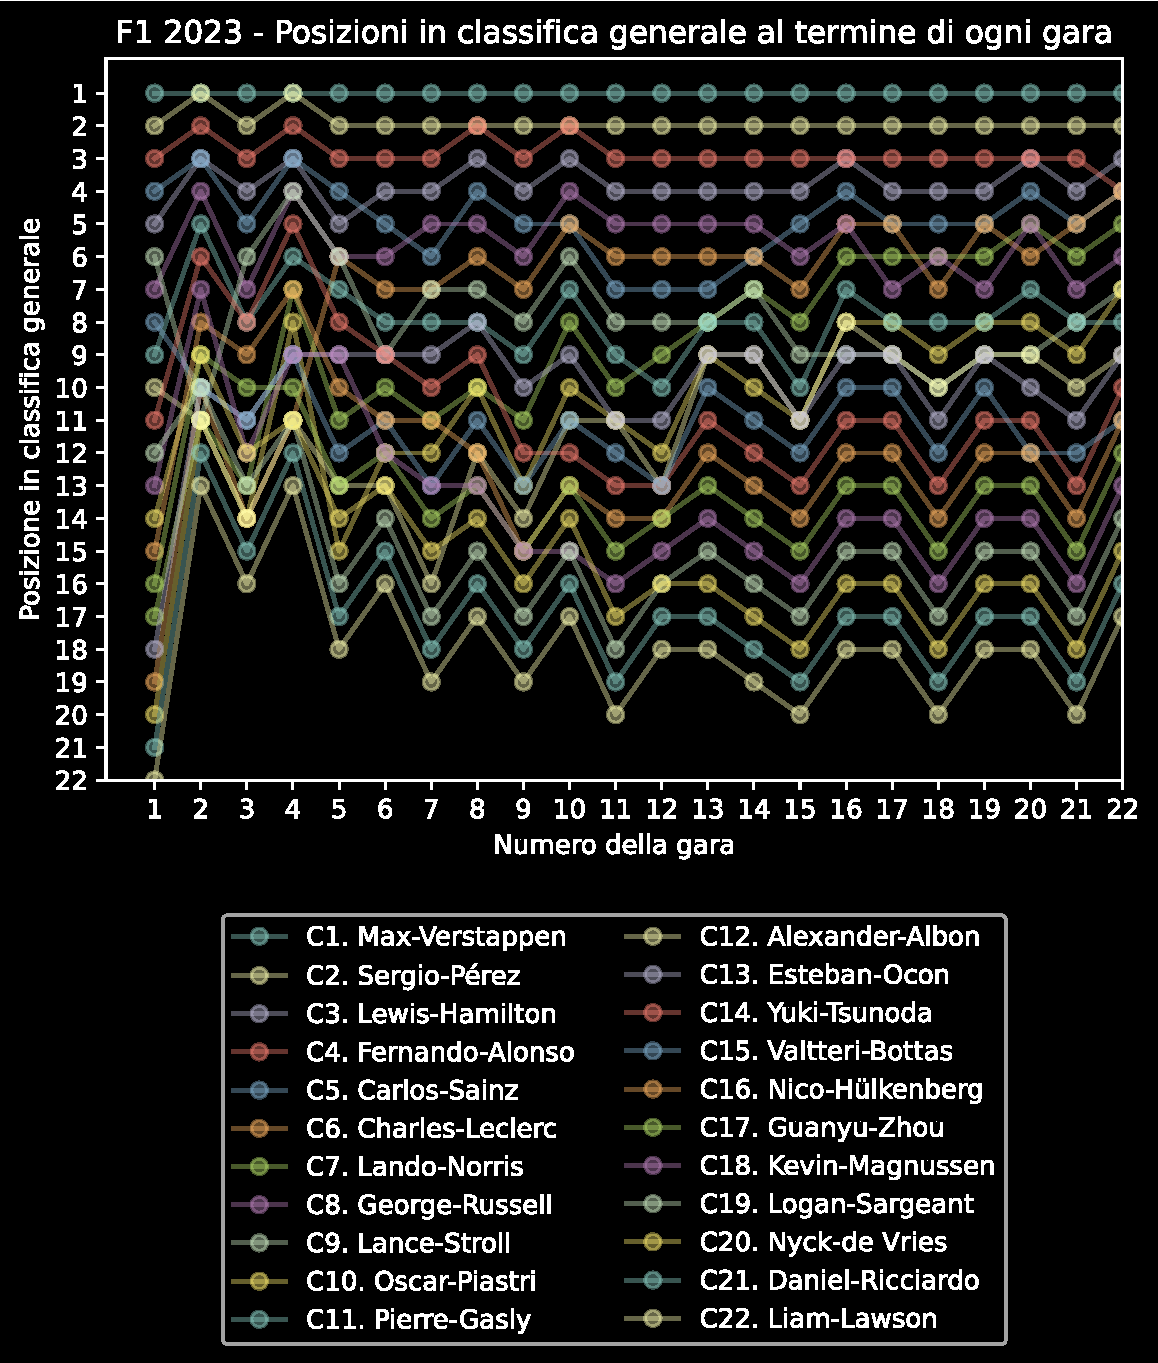
\includegraphics[width=\linewidth]{figures/condorcetstandings2023.pdf}
     \caption{Rappresentazione grafica della tabella \ref{table:classifichegeneralicondorcet2023tabella} }
     \label{fig:classifichegeneralicondorcet2023figura}
 \end{figure}


 \begin{table}[H]
    \centering
    \begingroup
    \resizebox{\linewidth}{!}{%
    \begin{tabular}{|c|c|c|c|c|c|c|c|c|c|c|c|c|c|c|c|c|c|c|c|c|c|c|}
  
    \hline
    \multicolumn{1}{|l|}{} & \multicolumn{1}{l|}{G1} & \multicolumn{1}{l|}{G2} & \multicolumn{1}{l|}{G3} & \multicolumn{1}{l|}{G4} & \multicolumn{1}{l|}{G5} & \multicolumn{1}{l|}{G6} & \multicolumn{1}{l|}{G7} & \multicolumn{1}{l|}{G8} & \multicolumn{1}{l|}{G9} & \multicolumn{1}{l|}{G10} & \multicolumn{1}{l|}{G11} & \multicolumn{1}{l|}{G12} & \multicolumn{1}{l|}{G13} & \multicolumn{1}{l|}{G14} & \multicolumn{1}{l|}{G15} & \multicolumn{1}{l|}{G16} & \multicolumn{1}{l|}{G17} & \multicolumn{1}{l|}{G18} & \multicolumn{1}{l|}{G19} & \multicolumn{1}{l|}{G20} & \multicolumn{1}{l|}{G21} & \multicolumn{1}{l|}{G22} \\ \hline
    C1. & 1 & 1 & 1 & 1 & 1 & 1 & 1 & 1 & 1 & 1 & 1 & 1 & 1 & 1 & 1 & 1 & 1 & 1 & 1 & 1 & 1 & 1 \\ \hline
C2. & 2 & 1 & 2 & 2 & 2 & 3 & 4 & 4 & 3 & 4 & 3 & 2 & 2 & 2 & 2 & 3 & 4 & 2 & 3 & 3 & 2 & 2 \\ \hline
C3.  & 5 & 3 & 4 & 4 & 4 & 4 & 3 & 3 & 4 & 3 & 2 & 3 & 3 & 3 & 3 & 2 & 2 & 4 & 2 & 2 & 3 & 3 \\ \hline
C4. & 3 & 2 & 3 & 3 & 3 & 2 & 2 & 2 & 2 & 2 & 2 & 4 & 2 & 3 & 4 & 4 & 3 & 3 & 4 & 4 & 4 & 4 \\ \hline
C5.  & 4 & 3 & 5 & 5 & 5 & 5 & 5 & 5 & 5 & 5 & 4 & 6 & 4 & 4 & 5 & 5 & 5 & 5 & 5 & 5 & 5 & 5 \\ \hline
C6.  & 19 & 8 & 16 & 9 & 9 & 8 & 8 & 7 & 7 & 7 & 6 & 7 & 6 & 6 & 6 & 6 & 6 & 8 & 8 & 8 & 8 & 8 \\ \hline
C7.  & 17 & 12 & 13 & 9 & 12 & 12 & 11 & 12 & 11 & 10 & 7 & 8 & 7 & 7 & 8 & 8 & 8 & 6 & 6 & 6 & 6 & 6 \\ \hline
C8.  & 7 & 4 & 6 & 6 & 6 & 6 & 6 & 6 & 6 & 6 & 5 & 5 & 5 & 5 & 7 & 7 & 7 & 7 & 7 & 7 & 7 & 7 \\ \hline
C9. & 6 & 8 & 7 & 6 & 7 & 11 & 9 & 10 & 9 & 8 & 8 & 9 & 8 & 8 & 10 & 11 & 11 & 11 & 11 & 11 & 11 & 11 \\ \hline
C10.  & 20 & 13 & 14 & 12 & 14 & 15 & 13 & 13 & 14 & 12 & 10 & 12 & 11 & 11 & 11 & 10 & 9 & 10 & 10 & 10 & 10 & 10 \\ \hline
C11.  & 9 & 5 & 8 & 8 & 8 & 7 & 7 & 8 & 8 & 9 & 9 & 10 & 9 & 9 & 9 & 9 & 10 & 9 & 9 & 9 & 9 & 9 \\ \hline
C12.  & 10 & 11 & 17 & 15 & 15 & 17 & 16 & 15 & 13 & 14 & 12 & 14 & 12 & 10 & 12 & 12 & 13 & 12 & 12 & 13 & 13 & 13 \\ \hline
C13.  & 18 & 8 & 13 & 13 & 11 & 9 & 9 & 9 & 10 & 11 & 11 & 11 & 10 & 11 & 13 & 13 & 12 & 13 & 13 & 12 & 12 & 12 \\ \hline
C14.  & 11 & 6 & 9 & 7 & 8 & 10 & 10 & 11 & 12 & 13 & 13 & 13 & 13 & 13 & 15 & 14 & 16 & 15 & 14 & 14 & 14 & 14 \\ \hline
C15. & 8 & 8 & 11 & 13 & 13 & 13 & 14 & 14 & 14 & 15 & 14 & 15 & 14 & 12 & 14 & 14 & 14 & 14 & 14 & 15 & 15 & 15 \\ \hline
C16.  & 15 & 9 & 10 & 10 & 12 & 15 & 14 & 16 & 15 & 17 & 16 & 17 & 16 & 15 & 17 & 16 & 17 & 17 & 16 & 17 & 17 & 17 \\ \hline
C17.  & 16 & 11 & 12 & 14 & 14 & 16 & 12 & 15 & 14 & 16 & 15 & 16 & 15 & 14 & 16 & 15 & 15 & 16 & 15 & 16 & 16 & 16 \\ \hline
C18.  & 13 & 7 & 13 & 11 & 10 & 14 & 15 & 17 & 16 & 18 & 17 & 18 & 17 & 16 & 18 & 17 & 18 & 18 & 17 & 18 & 18 & 18 \\ \hline
C19.  & 12 & 10 & 15 & 15 & 16 & 19 & 18 & 19 & 18 & 20 & 18 & 19 & 18 & 17 & 19 & 18 & 19 & 19 & 18 & 19 & 19 & 19 \\ \hline
C20.  & 14 & 10 & 14 & 16 & 17 & 18 & 17 & 18 & 17 & 19 & 18 & 20 & 19 & 18 & 20 & 19 & 20 & 20 & 19 & 20 & 20 & 21 \\ \hline
C21.  & 21 & 14 & 18 & 17 & 18 & 20 & 19 & 20 & 19 & 21 & 19 & 21 & 20 & 19 & 22 & 21 & 22 & 22 & 21 & 21 & 21 & 20 \\ \hline
C22.  & 22 & 15 & 19 & 18 & 19 & 21 & 20 & 21 & 20 & 22 & 20 & 22 & 21 & 20 & 21 & 20 & 21 & 21 & 20 & 22 & 22 & 22 \\ \hline
    \end{tabular}}
    \endgroup
    \caption{Tabella relativa al Mondiale F1 2023, in cui per ogni gara (G*)  è riportata la posizione del concorrente (C*) in classifica, al termine della gara stessa.
    I valori sono ricavati dall'applicazione dell'algoritmo di Schultze al termine di ogni gara, considerando anche le precedenti.
    Ogni gara rappresenta un voto, composto dagli ordini di arrivo.
    }
    \label{table:classifichegeneralischultze2023tabella}
\end{table}
\begin{figure}[H]
    \centering
     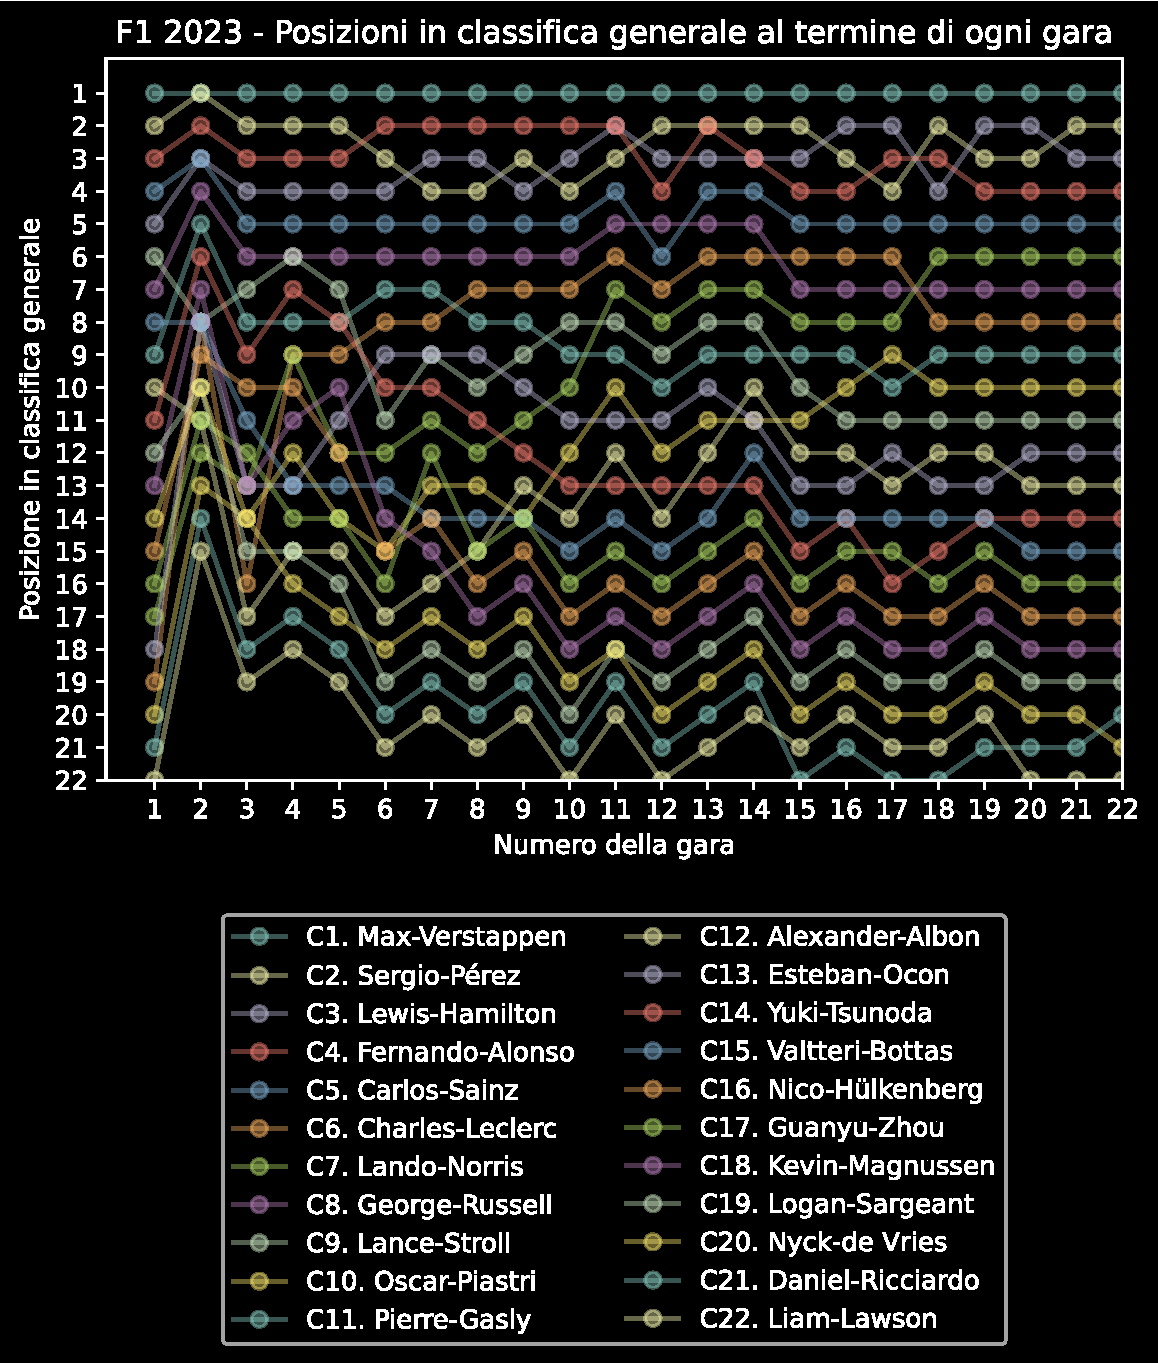
\includegraphics[width=\linewidth]{figures/schultzestandings2023.pdf}
     \caption{Rappresentazione grafica della tabella \ref{table:classifichegeneralischultze2023tabella} }
     \label{fig:classifichegeneralischultze2023figura}
 \end{figure}
 Si può notare che entrambi gli algoritmi impiegati tendono ad una soluzione che porta i concorrenti ad essere
 molto simili come posizionamento nelle prime fasi del campionato, causando numerosi pareggi ma proseguendo con le gare
 questi tendono a ridursi per via del numero incrementale di voti. Tuttavia, i risultati evidenziati da Condorcet 
 nell'ultima classifica manifestano numerosi pareggi, mentre Schultze riesce a discriminare in maniera più accurata
 gli esiti.
 In tabella \ref{table:distanzef12023} vengono mostrati i valori di distanza ottenuti applicando la 
 \textit{norma di Frobenius} alla differenza delle matrici rappresentate nelle prime due colonne.
 Si può notare che l'insieme delle classifiche generate sono significativamente diverse dall'insieme delle classifiche reali,
 mentre se ci si focalizza sulle classifiche finali la distanza è minore ma i valori generati da 
 Condorcet continuano a distinguersi maggiormente, soprattutto a causa dei pareggi, che nella classifica finale reale
 non sono presenti.
 \begin{table}[H]
    \centering
    \begingroup
    \resizebox{\linewidth}{!}{%
    \begin{tabular}{|c|c|c|}
    \hline
    \multicolumn{1}{|l|}{Elemento 1} & \multicolumn{1}{l|}{Elemento 2} & \multicolumn{1}{l|}{Valore distanza euclidea} \\ \hline
    Matrice "reale" & Matrice Condorcet &  68.23 \\ \hline
    Matrice "reale" & Matrice Schultze &  44.72 \\ \hline
   % Matrice Condorcet & Matrice Schultze &  48.04 \\ \hline
    Classifica finale "reale" & Classifica finale Condorcet &  14.35 \\ \hline
    Classifica finale "reale" & Classifica finale Schultze &  8.31 \\ \hline
    %Classifica finale Condorcet & Classifica finale Schultze &  14.04 \\ \hline
    \end{tabular}}
    \endgroup
    \caption{Campionato F1 2023 - Valori di distanza ottenuti applicando la 
    \textit{norma di Frobenius} alla differenza delle matrici rappresentate nelle prime due colonne.
    }
    \label{table:distanzef12023}
\end{table}
\section{Elaborazione del mondiale F1 2008}
È stata effettuata l'elaborazione del mondiale F1 2008, che rispetto al mondiale 2023 ha visto
una maggior competizione tra i concorrenti per le prime posizioni. Si è provveduto a generare le classifiche provvisorie 
replicando il flusso rappresentato nel paragrafo \ref{paragrafoelaborazionemondiale}.
Si riporta in tabella \ref{table:classifichefinali2008} la classifica finale reale ed i risultati ottenuti nelle
classifiche finali, usando l'algoritmo di Condorcet e l'algoritmo di Schultze.
%%2008
\begin{table}[H]
    \centering
    \begingroup
    \resizebox{\linewidth}{!}{%
    \begin{tabular}{|p{0.1\linewidth}|p{0.33\linewidth}|p{0.33\linewidth}|p{0.33\linewidth}|}
    \hline
    \multicolumn{1}{|l|}{Posizione} & \multicolumn{1}{l|}{Reali} & \multicolumn{1}{l|}{Condorcet} & \multicolumn{1}{l|}{Schultze} \\ \hline
    
    1. &	Lewis-Hamilton & 	 Felipe-Massa (C1.)& 	 Lewis-Hamilton 	 \\ \hline
    2.&	Felipe-Massa & 	 Lewis-Hamilton (C2.)& 	 Robert-Kubica 	 \\ \hline
    3.&	Kimi-Räikkönen & 	 Kimi-Räikkönen (C3.)\newline Robert-Kubica (C4.)& 	 Felipe-Massa 	 \\ \hline
    4.&	Robert-Kubica & 	 Nick-Heidfeld (C5.)& 	 Nick-Heidfeld 	 \\ \hline
    5.&	Fernando-Alonso & 	 Heikki-Kovalainen (C6.)& 	 Kimi-Räikkönen 	 \\ \hline
    6.&	Nick-Heidfeld & 	 Fernando-Alonso (C7.) & 	 Fernando-Alonso 	 \\ \hline
    7.&	Heikki-Kovalainen & 	 Jarno-Trulli (C8.)& 	 Heikki-Kovalainen 	 \\ \hline
    8.&	Sebastian-Vettel & 	 Timo-Glock (C9.)\newline Mark-Webber (C10.) & 	 Jarno-Trulli 	 \\ \hline
    9.&	Jarno-Trulli & 	 Nico-Rosberg (C11.)\newline Sebastian-Vettel (C12.) & 	 Mark-Webber 	 \\ \hline
    10.&	Timo-Glock & 	 David-Coulthard (C13.) & 	 Timo-Glock 	 \\ \hline
    11.	&Mark-Webber & 	 Kazuki-Nakajima (C14.)\newline Rubens-Barrichello (C15.) & 	 Nico-Rosberg 	 \\ \hline
    12.	&Nelson-Piquet Jr. & 	 Sébastien-Bourdais (C16.) \newline Nelson-Piquet Jr. (C17.)\newline Jenson-Button (C18.) & 	 Sebastian-Vettel 	 \\ \hline
    13.&	Nico-Rosberg & 	 Giancarlo-Fisichella (C19.) & 	 Kazuki-Nakajima 	 \\ \hline
    14.	&Rubens-Barrichello & 	 Adrian-Sutil (C20.)& 	 Nelson-Piquet Jr. 	 \\ \hline
    15.&	Kazuki-Nakajima & 	 Takuma-Sato (C21.) & 	 David-Coulthard 	 \\ \hline
    16.&	David-Coulthard & 	 Anthony-Davidson (C22.)& 	 Jenson-Button 	 \\ \hline
    17.&	Sébastien-Bourdais & 	 Assente & 	 Rubens-Barrichello 	 \\ \hline
    18.&	Jenson-Button & 	 Assente & 	 Sébastien-Bourdais 	 \\ \hline
    19.&	Giancarlo-Fisichella & 	 Assente & 	 Giancarlo-Fisichella 	 \\ \hline
    20.&	Adrian-Sutil & 	 Assente & 	 Adrian-Sutil 	 \\ \hline
    21.&	Takuma-Sato & 	 Assente & 	 Takuma-Sato 	 \\ \hline
    22.&	Anthony-Davidson & 	 Assente & 	 Anthony-Davidson 	 \\ \hline
    
    \end{tabular}}
    \endgroup
    \caption{Classifica finale reale e classifiche finali ottenute con 
    l'algoritmo di Condorcet e l'algoritmo di Schultze, relativamente al mondiale F1 2008 }
    \label{table:classifichefinali2008}
\end{table}
Nelle tabelle \ref{table:classifichegeneralireali2008tabella}, \ref{table:classifichegeneralicondorcet2008tabella} e \ref{table:classifichegeneralischultze2008tabella}
vengono mostrate le matrici complete con il posizionamento dei piloti in ogni classifica provvisoria.
Per motivi prettamente grafici, a ciascun concorrente è stato assegnato un acronimo, consultabile nella terza colonna della tabella \ref{table:classifichefinali2008}
Infine, per ciascuna tabella è stato generato il relativo grafico, nel quale le linee rappresentano i concorrenti,
l'asse delle ascisse rappresenta il numero sequenziale della gara e l'asse delle ordinate è associato al posizionamento in classifica
al termine della relativa gara.
Per la tabella \ref{table:classifichegeneralireali2008tabella} il grafico di riferimento è in figura \ref{fig:classifichegeneralireali2008figura},
mentre per le tabelle \ref{table:classifichegeneralicondorcet2008tabella} e \ref{table:classifichegeneralischultze2008tabella} i grafici sono rispettivamente
in figura \ref{fig:classifichegeneralicondorcet2008figura} ed in figura \ref{fig:classifichegeneralischultze2008figura}.
\begin{table}[H]
    \centering
    \begingroup
    \resizebox{\linewidth}{!}{%
    \begin{tabular}{|c|c|c|c|c|c|c|c|c|c|c|c|c|c|c|c|c|c|c|}
    \hline
    \multicolumn{1}{|l|}{} & \multicolumn{1}{l|}{G1} & \multicolumn{1}{l|}{G2} & \multicolumn{1}{l|}{G3} & \multicolumn{1}{l|}{G4} & \multicolumn{1}{l|}{G5} & \multicolumn{1}{l|}{G6} & \multicolumn{1}{l|}{G7} & \multicolumn{1}{l|}{G8} & \multicolumn{1}{l|}{G9} & \multicolumn{1}{l|}{G10} & \multicolumn{1}{l|}{G11} & \multicolumn{1}{l|}{G12} & \multicolumn{1}{l|}{G13} & \multicolumn{1}{l|}{G14} & \multicolumn{1}{l|}{G15} & \multicolumn{1}{l|}{G16} & \multicolumn{1}{l|}{G17} & \multicolumn{1}{l|}{G18} \\ \hline
    C1. & 8 & 18 & 6 & 4 & 2 & 3 & 3 & 1 & 2 & 2 & 3 & 2 & 2 & 2 & 2 & 2 & 2 & 2 \\ \hline
    C2. & 1 & 1 & 3 & 2 & 3 & 1 & 2 & 4 & 1 & 1 & 1 & 1 & 1 & 1 & 1 & 1 & 1 & 1 \\ \hline
    C3. & 8 & 2 & 1 & 1 & 1 & 2 & 4 & 3 & 3 & 3 & 2 & 3 & 4 & 4 & 4 & 4 & 4 & 3 \\ \hline
    C4. & 8 & 5 & 4 & 3 & 4 & 4 & 1 & 2 & 4 & 4 & 4 & 4 & 3 & 3 & 3 & 3 & 3 & 4 \\ \hline
    C5. & 2 & 3 & 2 & 5 & 5 & 5 & 5 & 5 & 5 & 5 & 5 & 6 & 5 & 5 & 5 & 5 & 5 & 6 \\ \hline
    C6. & 5 & 4 & 5 & 6 & 6 & 6 & 6 & 6 & 6 & 6 & 6 & 5 & 6 & 6 & 6 & 6 & 7 & 7 \\ \hline
    C7. & 4 & 7 & 9 & 10 & 8 & 8 & 9 & 9 & 9 & 9 & 8 & 8 & 8 & 7 & 7 & 7 & 6 & 5 \\ \hline
    C8. & 8 & 8 & 7 & 7 & 9 & 9 & 8 & 7 & 7 & 7 & 7 & 7 & 7 & 8 & 9 & 9 & 9 & 9 \\ \hline
    C9. & 8 & 18 & 14 & 14 & 15 & 17 & 13 & 13 & 14 & 16 & 10 & 10 & 10 & 11 & 10 & 11 & 10 & 10 \\ \hline
    C10. & 8 & 11 & 10 & 8 & 7 & 7 & 7 & 8 & 8 & 8 & 9 & 9 & 9 & 10 & 11 & 10 & 11 & 11 \\ \hline
    C11. & 3 & 6 & 8 & 9 & 10 & 10 & 10 & 10 & 11 & 12 & 13 & 13 & 14 & 14 & 12 & 13 & 13 & 13 \\ \hline
    C12.  & 8 & 18 & 21 & 21 & 22 & 12 & 14 & 14 & 15 & 15 & 16 & 14 & 12 & 9 & 8 & 8 & 8 & 8 \\ \hline
    C13.  & 8 & 12 & 13 & 15 & 14 & 16 & 12 & 12 & 13 & 14 & 15 & 16 & 16 & 16 & 16 & 16 & 16 & 16 \\ \hline
    C14.  & 6 & 9 & 11 & 11 & 11 & 11 & 11 & 11 & 12 & 13 & 14 & 15 & 15 & 15 & 15 & 15 & 15 & 15 \\ \hline
    C15.  & 8 & 16 & 16 & 17 & 17 & 14 & 15 & 15 & 10 & 10 & 12 & 12 & 13 & 13 & 14 & 14 & 14 & 14 \\ \hline
    C16.  & 7 & 10 & 12 & 13 & 13 & 15 & 17 & 18 & 17 & 18 & 18 & 18 & 17 & 17 & 17 & 17 & 17 & 17 \\ \hline
    C17.  & 8 & 14 & 17 & 18 & 18 & 19 & 19 & 17 & 18 & 11 & 11 & 11 & 11 & 12 & 13 & 12 & 12 & 12 \\ \hline
    C18.    & 8 & 13 & 15 & 12 & 12 & 13 & 16 & 16 & 16 & 17 & 17 & 17 & 18 & 18 & 18 & 18 & 18 & 18 \\ \hline
    C19.  & 8 & 15 & 18 & 16 & 16 & 18 & 18 & 19 & 19 & 19 & 19 & 19 & 19 & 19 & 19 & 19 & 19 & 19 \\ \hline
    C20. & 8 & 18 & 21 & 21 & 21 & 22 & 22 & 22 & 22 & 21 & 21 & 21 & 20 & 20 & 20 & 20 & 20 & 20 \\ \hline
    C21. & 8 & 18 & 20 & 19 & 19 & 20 & 20 & 20 & 20 & 20 & 20 & 20 & 21 & 21 & 21 & 21 & 21 & 21 \\ \hline
    C22.  & 8 & 17 & 19 & 20 & 20 & 21 & 21 & 21 & 21 & 22 & 22 & 22 & 22 & 22 & 22 & 22 & 22 & 22 \\ \hline
    \end{tabular}}
    \endgroup
    
    \caption{Tabella relativa al Mondiale F1 2008, in cui per ogni gara (G*)  è riportata la posizione del concorrente (C*) in classifica generale, al termine della gara stessa.
    I valori sono ricavati da Ergast API .}
    \label{table:classifichegeneralireali2008tabella}
\end{table}

\begin{figure}[H]
    \centering
     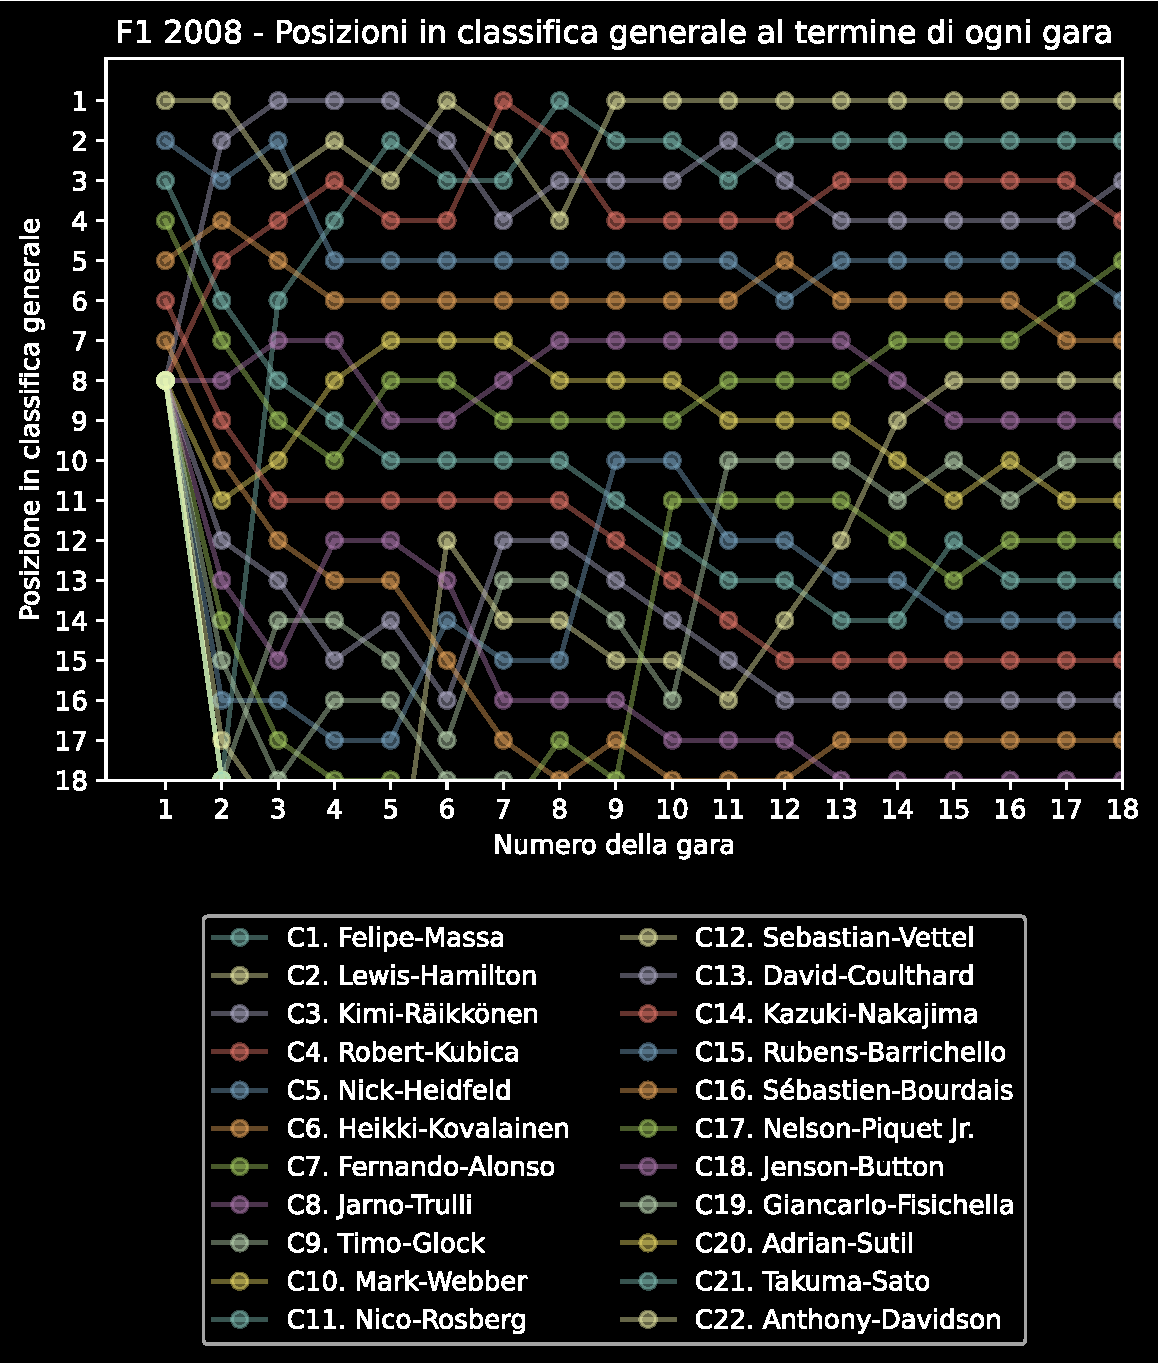
\includegraphics[width=\linewidth]{figures/realstandings2008.pdf}
     \caption{Rappresentazione grafica della tabella \ref{table:classifichegeneralireali2008tabella} }
     \label{fig:classifichegeneralireali2008figura}
 \end{figure}
 \begin{table}[H]
    \centering
    \begingroup
    \resizebox{\linewidth}{!}{%
    \begin{tabular}{|c|c|c|c|c|c|c|c|c|c|c|c|c|c|c|c|c|c|c|}
    \hline
    \multicolumn{1}{|l|}{} & \multicolumn{1}{l|}{G1} & \multicolumn{1}{l|}{G2} & \multicolumn{1}{l|}{G3} & \multicolumn{1}{l|}{G4} & \multicolumn{1}{l|}{G5} & \multicolumn{1}{l|}{G6} & \multicolumn{1}{l|}{G7} & \multicolumn{1}{l|}{G8} & \multicolumn{1}{l|}{G9} & \multicolumn{1}{l|}{G10} & \multicolumn{1}{l|}{G11} & \multicolumn{1}{l|}{G12} & \multicolumn{1}{l|}{G13} & \multicolumn{1}{l|}{G14} & \multicolumn{1}{l|}{G15} & \multicolumn{1}{l|}{G16} & \multicolumn{1}{l|}{G17} & \multicolumn{1}{l|}{G18}  \\ \hline
    C1.  & 13 & 12 & 8 & 6 & 2 & 2 & 1 & 1 & 1 & 1 & 1 & 1 & 1 & 1 & 1 & 1 & 1 & 1 \\ \hline
    C2.  & 1 & 1 & 4 & 3 & 3 & 1 & 2 & 3 & 3 & 2 & 1 & 2 & 2 & 2 & 2 & 1 & 2 & 2 \\ \hline
    C3.  & 8 & 4 & 1 & 1 & 1 & 1 & 1 & 1 & 2 & 2 & 1 & 3 & 3 & 5 & 5 & 4 & 3 & 3 \\ \hline
    C4.  & 9 & 5 & 2 & 2 & 4 & 2 & 3 & 2 & 4 & 3 & 2 & 3 & 3 & 3 & 3 & 2 & 3 & 3 \\ \hline
    C5.  & 2 & 2 & 3 & 3 & 5 & 3 & 4 & 3 & 5 & 4 & 3 & 4 & 4 & 4 & 3 & 3 & 4 & 4 \\ \hline
    C6.  & 5 & 3 & 3 & 4 & 9 & 5 & 5 & 4 & 6 & 5 & 4 & 4 & 5 & 4 & 4 & 3 & 5 & 5 \\ \hline
    C7.  & 4 & 5 & 6 & 5 & 8 & 6 & 9 & 6 & 9 & 8 & 7 & 7 & 8 & 7 & 6 & 5 & 6 & 6 \\ \hline
    C8.  & 15 & 7 & 4 & 4 & 6 & 6 & 6 & 4 & 7 & 6 & 5 & 5 & 6 & 6 & 7 & 6 & 7 & 7 \\ \hline
    C9. & 10 & 13 & 7 & 7 & 11 & 8 & 11 & 8 & 11 & 10 & 9 & 9 & 9 & 8 & 9 & 8 & 9 & 8 \\ \hline
    C10.  & 17 & 9 & 5 & 4 & 7 & 4 & 7 & 5 & 8 & 7 & 6 & 6 & 7 & 7 & 8 & 7 & 8 & 8 \\ \hline
    C11.  & 3 & 6 & 5 & 6 & 7 & 7 & 8 & 7 & 10 & 9 & 8 & 8 & 10 & 9 & 10 & 9 & 10 & 9 \\ \hline
    C12.  & 20 & 13 & 16 & 13 & 19 & 14 & 19 & 14 & 16 & 13 & 13 & 13 & 13 & 11 & 12 & 10 & 10 & 9 \\ \hline
    C13.  & 14 & 8 & 9 & 8 & 12 & 9 & 12 & 7 & 12 & 10 & 10 & 10 & 11 & 10 & 11 & 11 & 11 & 10 \\ \hline
    C14. & 6 & 9 & 7 & 7 & 11 & 8 & 11 & 10 & 11 & 10 & 11 & 12 & 12 & 11 & 12 & 12 & 12 & 11 \\ \hline
    C15.  & 22 & 13 & 12 & 9 & 13 & 10 & 13 & 8 & 13 & 10 & 11 & 11 & 12 & 13 & 14 & 14 & 12 & 11 \\ \hline
    C16.  & 7 & 13 & 9 & 10 & 14 & 13 & 16 & 12 & 15 & 13 & 13 & 13 & 13 & 13 & 14 & 14 & 13 & 12 \\ \hline
    C17.  & 12 & 8 & 10 & 11 & 16 & 11 & 14 & 11 & 15 & 12 & 12 & 12 & 13 & 13 & 15 & 14 & 10 & 12 \\ \hline
    C18. & 18 & 10 & 15 & 11 & 10 & 8 & 10 & 9 & 14 & 11 & 11 & 11 & 12 & 12 & 13 & 13 & 14 & 12 \\ \hline
    C19.  & 21 & 12 & 11 & 8 & 13 & 12 & 15 & 12 & 16 & 14 & 14 & 14 & 14 & 14 & 16 & 15 & 15 & 13 \\ \hline
    C20.  & 16 & 13 & 14 & 12 & 18 & 13 & 17 & 13 & 16 & 15 & 15 & 15 & 15 & 15 & 17 & 16 & 16 & 14 \\ \hline
    C21. & 11 & 11 & 13 & 10 & 15 & 12 & 16 & 13 & 17 & 16 & 16 & 16 & 16 & 16 & 18 & 17 & 17 & 15 \\ \hline
    C22.  & 19 & 12 & 13 & 11 & 17 & 13 & 18 & 14 & 18 & 17 & 17 & 17 & 17 & 17 & 19 & 18 & 18 & 16 \\ \hline
    \end{tabular}}
    \endgroup
    \caption{Tabella relativa al Mondiale F1 2008, in cui per ogni gara (G*)  è riportata la posizione del concorrente (C*) in classifica generale, al termine della gara stessa.
    I valori sono ricavati dall'applicazione dell'algoritmo di Condorcet al termine di ogni gara, considerando anche le precedenti.
    Ogni gara rappresenta un voto, composto dagli ordini di arrivo.
    }
    \label{table:classifichegeneralicondorcet2008tabella}
\end{table}
\begin{figure}[H]
    \centering
     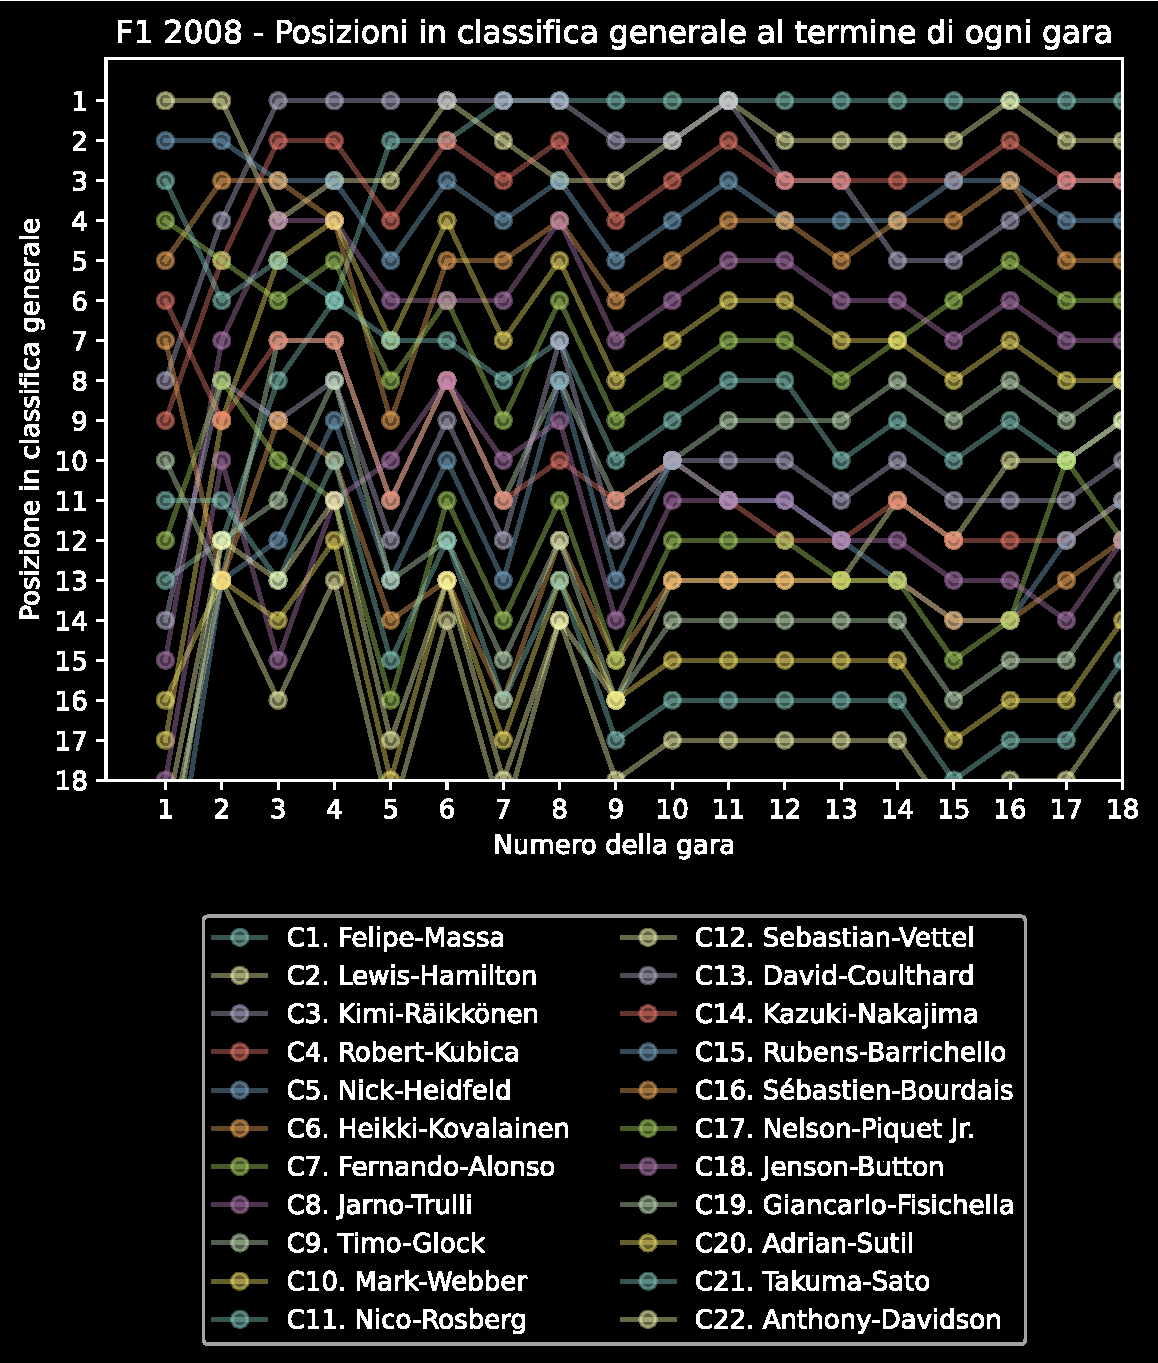
\includegraphics[width=\linewidth]{figures/condorcetstandings2008.pdf}
     \caption{Rappresentazione grafica della tabella \ref{table:classifichegeneralicondorcet2008tabella} }
     \label{fig:classifichegeneralicondorcet2008figura}
 \end{figure}
\begin{table}[H]
    \centering
    \begingroup
    \resizebox{\linewidth}{!}{%
    \begin{tabular}{|c|c|c|c|c|c|c|c|c|c|c|c|c|c|c|c|c|c|c|}

    \hline
    \multicolumn{1}{|l|}{} & \multicolumn{1}{l|}{G1} & \multicolumn{1}{l|}{G2} & \multicolumn{1}{l|}{G3} & \multicolumn{1}{l|}{G4} & \multicolumn{1}{l|}{G5} & \multicolumn{1}{l|}{G6} & \multicolumn{1}{l|}{G7} & \multicolumn{1}{l|}{G8} & \multicolumn{1}{l|}{G9} & \multicolumn{1}{l|}{G10} & \multicolumn{1}{l|}{G11} & \multicolumn{1}{l|}{G12} & \multicolumn{1}{l|}{G13} & \multicolumn{1}{l|}{G14} & \multicolumn{1}{l|}{G15} & \multicolumn{1}{l|}{G16} & \multicolumn{1}{l|}{G17} & \multicolumn{1}{l|}{G18}  \\ \hline
    C1.  & 13 & 14 & 9 & 7 & 5 & 3 & 3 & 3 & 5 & 4 & 6 & 5 & 3 & 3 & 4 & 4 & 4 & 3 \\ \hline
    C2.  & 1 & 1 & 5 & 4 & 3 & 2 & 3 & 4 & 3 & 3 & 3 & 2 & 1 & 2 & 1 & 2 & 1 & 1 \\ \hline
    C3.  & 8 & 3 & 1 & 1 & 1 & 1 & 2 & 2 & 2 & 2 & 1 & 3 & 6 & 6 & 6 & 6 & 5 & 5 \\ \hline
    C4.  & 9 & 4 & 4 & 2 & 2 & 1 & 1 & 1 & 1 & 1 & 2 & 1 & 2 & 1 & 2 & 1 & 2 & 2 \\ \hline
    C5.  & 2 & 2 & 2 & 3 & 4 & 4 & 2 & 5 & 4 & 4 & 4 & 6 & 4 & 4 & 3 & 3 & 3 & 4 \\ \hline
    C6.  & 5 & 2 & 3 & 5 & 6 & 6 & 4 & 6 & 6 & 5 & 5 & 4 & 5 & 5 & 5 & 5 & 7 & 7 \\ \hline
    C7.  & 4 & 5 & 6 & 9 & 7 & 7 & 6 & 8 & 9 & 7 & 8 & 9 & 8 & 8 & 7 & 7 & 6 & 6 \\ \hline
    C8.  & 15 & 7 & 7 & 6 & 7 & 8 & 5 & 7 & 7 & 6 & 7 & 7 & 7 & 7 & 8 & 8 & 8 & 8 \\ \hline
    C9.  & 10 & 13 & 11 & 12 & 11 & 11 & 8 & 10 & 11 & 10 & 11 & 11 & 10 & 10 & 10 & 11 & 10 & 10 \\ \hline
    C10. & 17 & 9 & 8 & 8 & 7 & 5 & 4 & 7 & 8 & 7 & 9 & 8 & 9 & 9 & 9 & 9 & 9 & 9 \\ \hline
    C11.  & 3 & 6 & 7 & 10 & 8 & 9 & 7 & 9 & 10 & 8 & 10 & 10 & 11 & 11 & 11 & 10 & 11 & 11 \\ \hline
    C12.  & 20 & 19 & 20 & 20 & 19 & 19 & 14 & 16 & 18 & 15 & 17 & 16 & 17 & 14 & 13 & 12 & 12 & 12 \\ \hline
    C13.  & 14 & 8 & 12 & 13 & 9 & 13 & 9 & 11 & 14 & 12 & 13 & 13 & 13 & 13 & 13 & 14 & 15 & 15 \\ \hline
    C14.  & 6 & 8 & 10 & 11 & 10 & 10 & 10 & 12 & 13 & 9 & 12 & 12 & 12 & 12 & 12 & 13 & 13 & 13 \\ \hline
    C15.  & 22 & 17 & 16 & 16 & 14 & 14 & 12 & 13 & 12 & 11 & 14 & 14 & 15 & 16 & 15 & 16 & 17 & 17 \\ \hline
    C16.  & 7 & 12 & 14 & 17 & 16 & 18 & 15 & 18 & 17 & 16 & 18 & 17 & 18 & 18 & 16 & 17 & 18 & 18 \\ \hline
    C17.  & 12 & 8 & 13 & 17 & 15 & 16 & 14 & 15 & 16 & 13 & 15 & 13 & 14 & 15 & 14 & 14 & 14 & 14 \\ \hline
    C18.  & 18 & 11 & 17 & 14 & 12 & 12 & 11 & 14 & 15 & 14 & 16 & 15 & 16 & 17 & 14 & 15 & 16 & 16 \\ \hline
    C19.  & 21 & 15 & 15 & 14 & 13 & 15 & 13 & 17 & 17 & 17 & 19 & 18 & 19 & 19 & 17 & 18 & 19 & 19 \\ \hline
    C20. & 16 & 18 & 19 & 19 & 18 & 20 & 17 & 20 & 20 & 18 & 20 & 19 & 20 & 20 & 18 & 19 & 20 & 20 \\ \hline
    C21.  & 11 & 10 & 14 & 15 & 15 & 17 & 16 & 19 & 19 & 19 & 21 & 20 & 21 & 21 & 19 & 20 & 21 & 21 \\ \hline
    C22.  & 19 & 16 & 18 & 18 & 17 & 21 & 18 & 21 & 21 & 20 & 22 & 21 & 22 & 22 & 20 & 21 & 22 & 22 \\ \hline
    \end{tabular}}
    \endgroup
    \caption{Tabella relativa al Mondiale F1 2008, in cui per ogni gara (G*)  è riportata la posizione del concorrente (C*) in classifica generale, al termine della gara stessa.
    I valori sono ricavati dall'applicazione dell'algoritmo di Schultze al termine di ogni gara, considerando anche le precedenti.
    Ogni gara rappresenta un voto, composto dagli ordini di arrivo.
    }
    \label{table:classifichegeneralischultze2008tabella}
\end{table}
\begin{figure}[H]
    \centering
     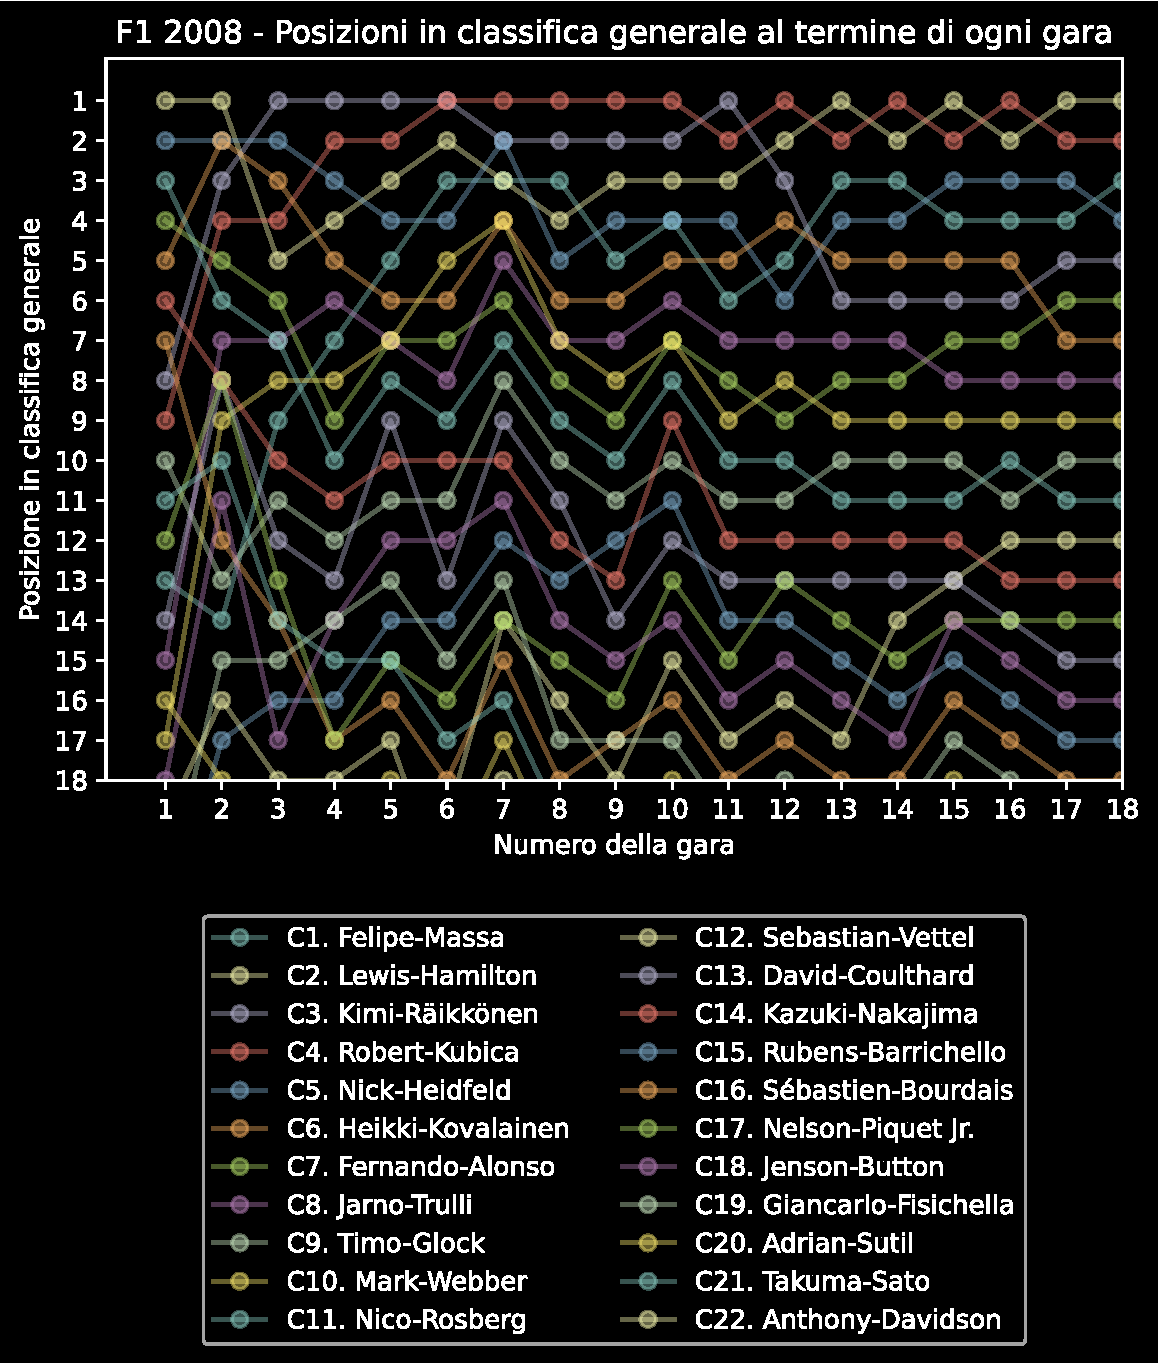
\includegraphics[width=\linewidth]{figures/schultzestandings2008.pdf}
     \caption{Rappresentazione grafica della tabella \ref{table:classifichegeneralischultze2008tabella} }
     \label{fig:classifichegeneralischultze2008figura}
 \end{figure}
 Gli algoritmi impiegati hanno permesso di elaborare una differente distribuzione della prima classifica provvisoria
 rispetto alla realtà, in cui molti piloti erano finiti fuori gara per incidenti o problemi di motore.
 Al pari del caso inerente al campionato 2023, si continua ad evidenziare una fase iniziale 
 con numerosi pareggi per poi distinguerli successivamente, tuttavia i risultati di Condorcet mostrano limiti in merito alla capacità
 di discriminazione di un vincitore unico per ogni posizione.
 In tabella \ref{table:distanzef12008} vengono mostrati i valori di distanza ottenuti applicando la 
 \textit{norma di Frobenius} alla distanza tra le matrici rappresentate nelle prime due colonne.
 Rispetto al caso del campionato 2023 si può notare un differenza più marcata in termini di distanze, sia nel caso
 di Schultze che in Condorcet. Quest'ultimo mostra una maggior differenza sia nel caso in cui viene confrontato
 l'insieme delle classifiche provvisorie, sia nel caso della classifica finale.
 \begin{table}[H]
    \centering
    \begingroup
    \resizebox{\linewidth}{!}{%
    \begin{tabular}{|c|c|c|}

    \hline
    \multicolumn{1}{|l|}{Elemento 1} & \multicolumn{1}{l|}{Elemento 2} & \multicolumn{1}{l|}{Valore distanza euclidea} \\ \hline
    Matrice "reale" & Matrice Condorcet &  77.19 \\ \hline
    Matrice "reale" & Matrice Schultze &  52.53 \\ \hline
    %Matrice Condorcet & Matrice Schultze &  55.94 \\ \hline
    Classifica finale "reale" & Classifica finale Condorcet &  24.6 \\ \hline
    Classifica finale "reale" & Classifica finale Schultze &  12.45 \\ \hline
    %Classifica finale Condorcet & Classifica finale Schultze &  19.34 \\ \hline
    \end{tabular}   }
    \endgroup
    \caption{Campionato F1 2008 - Valori di distanza ottenuti applicando la 
    \textit{norma di Frobenius} alla differenza delle matrici rappresentate nelle prime due colonne.
    }
    \label{table:distanzef12008}
\end{table}
%----------------------------------------------------------------------------------------
\chapter{Conclusioni}
In questa tesi è stata presentata un'introduzione sulla \textit{democrazia} e sullo stato attuale 
della \textit{democrazia digitale}, illustrando soluzioni esistenti sia nell'ambito delle decisioni
politiche, sia nell'ambito di contesti logistici che impattano la quotidianità della popolazione.
È stata presentata la creazione di una libreria multipiattaforma in \texttt{Kotlin Multiplatform},
avente lo scopo di rendere disponibile uno strumento per gestire le votazioni digitali, parametrandole
come ritenuto più opportuno dall'utilizzatore finale, ossia dall'organizzatore della votazione.
Questa libreria è stata  progettata ponendo l'accento su una tecnologia multipiattaforma per 
massimizzarne la diffusione su differenti sistemi, assicurando la piena compatibilità con gli stessi.
È stata svolta l'analisi del modello del dominio da trattare, in particolare si è reso evidente
che esistono due tipologie principali di voto che caratterizzano una possibile votazione.
Sono stati ideati dei \ac{dsl} utili a semplificare la definizione e la struttura di un pool delle votazioni,
riportando per essi i diagrammi UML architetturali.
Successivamente sono stati descritti i passi implementativi salienti, corredati dai test effettuati
e dagli strumenti utilizzati nel contesto di \textit{build automation}.
Riguardo a questi ultimi, sono stati illustrati gli step realizzati per arrivare alla generazione
e pubblicazione degli artefatti finali, compresa la documentazione a corredo.
Infine viene mostrata un'estensione dei casi studio, applicando le funzionalità realizzate a
dati reali relativi ai campionati \ac{f1}.
Per questi ultimi vengono approfonditi i dettagli relativi alle classifiche ricalcolate utilizzando
la libreria e vengono posti a confronto con i dati reali, misurando le differenze tramite un'opportuna
metrica di distanza. La possibilità di ottenere dei pareggi nelle classifiche generate, ha permesso di
ottenere una maggior espressività sul piazzamento dei concorrenti, ma allo stesso tempo ha comportato 
una maggior distanza rispetto alle classifiche reali, che non riportavano la possibilità di pareggio.
Le future implementazioni possono consistere nella gestione di eventi sportivi che riportano una
struttura più complessa, ad esempio l'adozione di gironi e tornei ad eliminazione diretta,
e secondo, ma non per importanza, l'estensione degli algoritmi disponibili sia per le votazioni a 
singola preferenza che per quelle a lista di preferenze.

%----------------------------------------------------------------------------------------
% BIBLIOGRAPHY
%----------------------------------------------------------------------------------------

\backmatter

\nocite{*} % comment this to only show the referenced entries from the .bib file 


\bibliographystyle{alpha}
\bibliography{bibliography}

\end{document}